\documentclass[11pt]{article}
\usepackage[margin=1in,a4paper]{geometry}
\usepackage[utf8]{inputenc}
\usepackage{hyperref}
\usepackage{amsmath,amssymb}
\usepackage{graphicx}
\usepackage{enumitem}
\usepackage{booktabs}
\usepackage{tabularx}
\usepackage[T1]{fontenc}
\usepackage{cmap}
\usepackage{inconsolata}
\usepackage{makecell}
\usepackage{pdfpages}
\usepackage{float}
\usepackage{xcolor}
\usepackage{listings}
\lstset{
  language=R,
  basicstyle=\ttfamily\small,
  keywordstyle=\color{blue},
  commentstyle=\color{gray},
  stringstyle=\color{teal},
  frame=single,
  numbers=none,
  keepspaces=true,
  columns=fullflexible,
  breaklines=false,
  showstringspaces=false
}
\setlist{nosep}

\newcommand{\noi}{\noindent}
\renewcommand\theadfont{\normalsize\bfseries}

\begin{document}

% Title page
\begin{titlepage}
\begin{center}
{\LARGE \textbf{ACTL30007 Actuarial Modelling III}}\\[1.5em]
{\Large Comprehensive Exam Review Notes}\\[10em]
{\large \textit{Student Name: Omar Amin}}\\[1em]
{\large Semester 1, 2025}
\end{center}
\end{titlepage}

\tableofcontents
\newpage

%%%%%%%%%%%%%%%%%%%%%%%%%%%%%%%%%%%%%%%%%%%%%%%%%%%%%%%%%%%%%%%%%%%%%%%%%%%%%%
\section{Module 1 – Introduction to General Insurance Modelling}
\subsection{Overview of General Insurance (GI)}
\noindent General Insurance (GI), also known as non-life or property \& casualty insurance, involves covering risks associated with losses (e.g., motor vehicle accidents, property damage, liability).\\
\noindent Unlike life insurance (where the primary event is death or survival, typically modelled by life tables and deterministic mortality laws), GI requires modelling both:
\begin{itemize}
  \item \textbf{Frequency} of claim occurrences (how many claims happen in a fixed period, e.g., one year).
  \item \textbf{Severity} of claim sizes (the monetary amount of each claim).
\end{itemize}
\noindent The general framework is the \textit{Collective Risk Model}, which defines the total loss \(S\) over a period as
\[
S \;=\; \sum_{i=1}^{N} X_i \,,
\]
where:
\begin{itemize}
  \item \(N\) is the random number of claims occurring in that period (the \textit{claim frequency}).
  \item \(X_1, X_2, \dots, X_N\) are the individual claim sizes (the \textit{claim severities}), assumed i.i.d.\ with common distribution \(F_X(x)\).
  \item We usually assume \(N\) is independent of the \(\{X_i\}\).
\end{itemize}
\noindent Key tasks in GI modelling:
\begin{enumerate}
  \item Estimate the distribution of \(N\) from historical claim counts (e.g., Poisson, Negative Binomial).
  \item Estimate the distribution of claim sizes \(X\) (e.g., Exponential, Gamma, Lognormal, Pareto).
  \item Compute or approximate the distribution of the aggregate loss \(S\).
  \item Use \(S\) to set premiums, calculate reserves, and assess risk metrics (e.g., Value-at-Risk, Tail Value-at-Risk).
\end{enumerate}
\noindent In this course, we also cover:
\begin{itemize}
  \item Dependence modelling via \textbf{copulas} (Module 5).
  \item \textbf{Extreme Value Theory (EVT)} for tail modelling (Module 6).
  \item \textbf{Time series methods} for modelling insurance data over time (Modules 7–10).
\end{itemize}

\subsection{Key Definitions and Notation}
\noindent Throughout these notes, we will use:
\begin{itemize}
  \item \(N\): claim count random variable (frequency).
  \item \(X\), \(X_i\): claim size (severity) random variable(s).
  \item \(S\): aggregate loss \(S=\sum_{i=1}^N X_i\).
  \item \(F_N(n)\), \(p_N(n) = \Pr(N=n)\): mass function or distribution of \(N\).
  \item \(F_X(x)\), \(f_X(x)\): CDF and density (or mass function) of \(X\).
  \item \(\mu_N = \mathbb{E}[N]\), \(\sigma_N^2 = \mathrm{Var}(N)\).
  \item \(\mu_X = \mathbb{E}[X]\), \(\sigma_X^2 = \mathrm{Var}(X)\).
  \item \(\mu_S, \sigma_S^2\): mean and variance of \(S\).
  \item \(M_X(t) = \mathbb{E}[e^{tX}]\): moment generating function (MGF) of \(X\).
  \item \(G_N(z) = \mathbb{E}[z^N]\): probability generating function (PGF) of \(N\).
\end{itemize}

\subsubsection{Moments of Aggregate Loss}
\noindent Under the assumption that \(N\) is independent of \(\{X_i\}\), we have:
\[
\mathbb{E}[S]
= \mathbb{E}\big[\mathbb{E}(S \mid N)\big]
= \mathbb{E}\big[N \cdot \mathbb{E}[X]\big]
= \mu_N \, \mu_X.
\]
\[
\mathrm{Var}(S)
= \mathbb{E}\big[\mathrm{Var}(S \mid N)\big]
+ \mathrm{Var}\big(\mathbb{E}[S \mid N]\big).
\]
\noindent Since \(\mathrm{Var}\big(\sum_{i=1}^N X_i \mid N\big) = N\,\sigma_X^2\) and \(\mathbb{E}[S \mid N] = N\,\mu_X\), we get:
\[
\mathrm{Var}(S)
= \mathbb{E}[N\,\sigma_X^2] + \mathrm{Var}(N\,\mu_X)
= \sigma_X^2\,\mu_N + \mu_X^2\,\sigma_N^2.
\]
\noindent Hence,
\[
\boxed{
\mathbb{E}[S] = \mu_N \,\mu_X, 
\quad
\mathrm{Var}(S) = \mu_N\,\sigma_X^2 + \mu_X^2\,\sigma_N^2.
}
\]

\subsubsection{MGF and PGF Relationship}
\noindent If \(G_N(z) = \mathbb{E}[z^N]\) is the PGF of \(N\), and \(M_X(t) = \mathbb{E}[e^{tX}]\) is the MGF of \(X\), then the MGF of \(S\) is:
\[
M_S(t)
= \mathbb{E}\big[e^{t \sum_{i=1}^N X_i}\big]
= \mathbb{E}\big[(M_X(t))^N\big]
= G_N\big(M_X(t)\big).
\]
\noindent For example, if \(N\sim \text{Poisson}(\lambda)\) then \(G_N(z)=\exp\big\{\lambda(z-1)\big\}\). Thus
\[
M_S(t) = \exp\big\{\lambda (M_X(t) - 1)\big\}.
\]
\noindent By expanding \(M_X(t)\) as \(1 + \mu_X t + \tfrac{1}{2}\mu_{X,2} t^2 + \cdots\), we recover the moments of \(S\) above.

\subsubsection*{R Code: Simulating a Collective Risk Model}
\begin{lstlisting}
# Simulate aggregate loss S = sum_{i=1}^N X_i, 
# where N ~ Poisson(lambda), X_i ~ Gamma(shape, scale)

lambda <- 3            # expected number of claims
shape <- 2; scale <- 1000  # Gamma parameters (mean = 2000)
nsim <- 100000
set.seed(2025)

S_sim <- numeric(nsim)
for(i in 1:nsim){
  N_i <- rpois(1, lambda)         # draw frequency
  if(N_i > 0){
    X_i <- rgamma(N_i, shape=shape, scale=scale)  # draw severities
    S_sim[i] <- sum(X_i)
  } else {
    S_sim[i] <- 0
  }
}
# Empirical mean and variance
mean(S_sim)  # ~ lambda * shape * scale = 3 * 2000 = 6000
var(S_sim)   # ~ lambda*(shape*scale^2 + shape^2*scale^2) 
\end{lstlisting}
\noindent \noindent The above code simulates \(10^5\) years of aggregated losses. We compare the sample mean and variance to theoretical values:
\[
\mathbb{E}[S] = \lambda \cdot \alpha\beta = 3 \times (2 \times 1000) = 6000,
\]
\[
\mathrm{Var}(S) = \lambda\big(\alpha\beta^2 + \alpha^2 \beta^2\big) 
= 3\big(2\times1000^2 + (2\times1000)^2\big) = 3(2\times10^6 + 4\times10^6) = 18\times10^6.
\]
\newpage
%%%%%%%%%%%%%%%%%%%%%%%%%%%%%%%%%%%%%%%%%%%%%%%%%%%%%%%%%%%%%%%%%%%%%%%%%%%%%%
\section{Module 2 – Collective Risk Modelling Theory}

\noi \textit{Note: this module was cut short since rest is not necessary for final exam, check mid semester revision sheet for more content or refer to lecture slides.}

\subsection{The Individual Risk Model}

\noi In the Individual Risk Model
\[
S \;=\; Y_{1} + \dots + Y_{n} \;=\; \sum_{i=1}^{n} Y_{i},
\]
\noi where \(Y_i,\;i=1,2,\dots,n,\) are iid claims.

\noi There are several methods to get probabilities about \(S\):
\begin{itemize}
  \item get the whole distribution of \(S\) (if possible)
    \begin{itemize}
      \item Convolutions
      \item Generating functions
    \end{itemize}
  \item approximate with the help of the moments of \(S\) (Module 4)
\end{itemize}

\subsubsection*{Convolutions Formulas}

\noi In short
\begin{itemize}
  \item discrete case:
    \begin{itemize}
      \item df: 
        \[
        F_{X+Y}(s)
        = \sum_x F_Y(s - x)\,f_X(x)
        \]
      \item pmf:
        \[
        f_{X+Y}(s)
        = \sum_x f_Y(s - x)\,f_X(x)
        \]
    \end{itemize}
  \item continuous case:
    \begin{itemize}
      \item cdf:
        \[
        F_{X+Y}(s)
        = \int_{-\infty}^{s} F_Y(s - x)\,f_X(x)\,dx
        \]
      \item pdf:
        \[
        f_{X+Y}(s)
        = \int_{-\infty}^{s} f_Y(s - x)\,f_X(x)\,dx
        \]
    \end{itemize}
\end{itemize}

\subsubsection{Convolution Example and basic R}
\noi Consider 3 discrete r.v.'s with probability mass functions
\[
f_1(y)=\begin{cases}
\tfrac{1}{4},&y=0,\\
\tfrac{1}{2},&y=1,\\
\tfrac{1}{4},&y=2,
\end{cases}
\quad
f_2(y)=\begin{cases}
\tfrac{1}{2},&y=0,\\
\tfrac{1}{2},&y=2,
\end{cases}
\quad
f_3(y)=\begin{cases}
\tfrac{1}{4},&y=0,\\
\tfrac{1}{2},&y=2,\\
\tfrac{1}{4},&y=4.
\end{cases}
\]
\noi Calculate the pmf \(f_{1+2+3}\) and the df \(F_{1+2+3}\) of the sum of the three random variables.

\noi
\begin{table}[ht]
\centering
\caption{Using convolutions}
\vspace{0.5em}
\begin{tabular}{|c|c|c|c|c|c|c|}
\hline
\(y\) & \(f_1(y)\) & \(f_2(y)\) & \(f_{1+2}(y)\) & \(f_3(y)\) & \(f_{1+2+3}(y)\) & \(F_{1+2+3}(y)\) \\
\hline
0 & \(\tfrac{1}{4}\) & \(\tfrac{1}{2}\) & \(\tfrac{1}{8}\) & \(\tfrac{1}{4}\) & \(\tfrac{1}{32}\) & \(\tfrac{1}{32}\) \\
1 & \(\tfrac{1}{2}\) & 0 & \(\tfrac{2}{8}\) & 0 & \(\tfrac{2}{32}\) & \(\tfrac{3}{32}\) \\
2 & \(\tfrac{1}{4}\) & \(\tfrac{1}{2}\) & \(\tfrac{2}{8}\) & \(\tfrac{1}{2}\) & \(\tfrac{4}{32}\) & \(\tfrac{7}{32}\) \\
3 & 0 & 0 & \(\tfrac{2}{8}\) & 0 & \(\tfrac{6}{32}\) & \(\tfrac{13}{32}\) \\
4 & 0 & 0 & \(\tfrac{1}{8}\) & \(\tfrac{1}{4}\) & \(\tfrac{6}{32}\) & \(\tfrac{19}{32}\) \\
5 & 0 & 0 & 0 & 0 & \(\tfrac{6}{32}\) & \(\tfrac{25}{32}\) \\
6 & 0 & 0 & 0 & 0 & \(\tfrac{4}{32}\) & \(\tfrac{29}{32}\) \\
7 & 0 & 0 & 0 & 0 & \(\tfrac{2}{32}\) & \(\tfrac{31}{32}\) \\
8 & 0 & 0 & 0 & 0 & \(\tfrac{1}{32}\) & \(\tfrac{32}{32}\) \\
\hline
\end{tabular}
\end{table}

\[
f_{1+2}(2)
= \tfrac{1}{4}\cdot\tfrac{1}{2}
+ \tfrac{1}{2}\cdot 0
+ \tfrac{1}{4}\cdot\tfrac{1}{2},
\]
\[
f_{1+2+3}(4)
= \tfrac{1}{8}\cdot\tfrac{1}{4}
+ \tfrac{2}{8}\cdot 0
+ \tfrac{2}{8}\cdot\tfrac{1}{2}
+ \tfrac{2}{8}\cdot 0
+ \tfrac{1}{8}\cdot\tfrac{1}{4}.
\]

\noi Contrary to Excel, convolutions are extremely easy to implement in R using vectors.

\begin{lstlisting}
f1 <- c(1/4, 1/2, 1/4, 0, 0)
f2 <- c(1/2, 0, 1/2, 0, 0)
f12 <- c(
  f1[1] * f2[1],
  sum(f1[1:2] * f2[2:1]),
  sum(f1[1:3] * f2[3:1]),
  sum(f1[1:4] * f2[4:1]),
  sum(f1[1:5] * f2[5:1])
)
f12

## [1] 0.125 0.250 0.250 0.250 0.125
\end{lstlisting}

\subsection{The Collective Risk Model}
\noi In the Collective Risk Model, aggregate losses become
\[
S \;=\; Y_{1} + \dots + Y_{N} \;=\; \sum_{i=1}^{N} Y_{i}.
\]
\noi This is a random sum. We make the following assumptions:
\begin{itemize}
  \item \(N \subset \mathbb{Z}_{\ge0}\) is the number of claims
  \item \(Y_i > 0\) is the amount of the \(i\)th claim
  \item the \(Y_i\)'s are iid with
    \begin{itemize}
      \item (c)df \(G(y)\)
      \item p(d/m)f \(g(y)\)
    \end{itemize}
  \item the \(Y_i\)'s and \(N\) are mutually independent
\end{itemize} \phantom{i}

\noi We have
\[
\mathbb{E}[S]
= \mathbb{E}\bigl[\mathbb{E}[S\mid N]\bigr]
= \mathbb{E}\bigl[N\,\mathbb{E}[Y]\bigr]
= \mathbb{E}[N]\,\mathbb{E}[Y],
\]
and
\[
\begin{aligned}
\text{Var}(S)
&= \mathbb{E}\bigl[\text{Var}(S\mid N)\bigr]
  + \text{Var}\bigl(\mathbb{E}[S\mid N]\bigr)\\
&= \mathbb{E}\bigl[N\,\text{Var}(Y)\bigr]
  + \text{Var}\bigl(N\,\mathbb{E}[Y]\bigr)\\
&= \mathbb{E}[N]\,\text{Var}(Y)
  + \mathbb{E}[Y]^2\,\text{Var}(N)\\
&= \mathbb{E}[N]\bigl(\mathbb{E}[Y^2]-\mathbb{E}[Y]^2\bigr)
  + \mathbb{E}[Y]^2\,\text{Var}(N)\\
&= \mathbb{E}[N]\,\mathbb{E}[Y^2]
  + \mathbb{E}[Y]^2\bigl(\text{Var}(N)-\mathbb{E}[N]\bigr).
\end{aligned}
\]

\noi The moment generating function of \(S\) is
\[
\begin{aligned}
M_S(t)
&= \mathbb{E}\bigl[e^{tS}\bigr]
= \mathbb{E}\Bigl[\mathbb{E}\bigl[e^{t(Y_1 + \dots + Y_N)}\mid N\bigr]\Bigr]\\
&= \mathbb{E}\bigl[M_Y(t)^N\bigr]
= \mathbb{E}\bigl[e^{N\ln M_Y(t)}\bigr]
= M_N\!\bigl(\ln M_Y(t)\bigr).
\end{aligned}
\]

\subsection{Distribution of \(S\)}

\noi It is possible to get a fairly general expression for the df of \(S\) by conditioning on the number of claims:
\[
F_S(x)
\;=\;
\sum_{n=0}^{\infty}\Pr[S \le x\mid N = n]\,\Pr[N = n]
\;=\;
\sum_{n=0}^{\infty}G^{*n}(x)\,\Pr[N = n]
\tag{1}
\]
\noi where \(G^{*n}(y)\) is the \(n\)th convolution of \(G\).  

\noi Note that
\begin{itemize}
  \item \(N\) will always be discrete, so this works for any type of rv \(Y\) (continuous, discrete or mixed).
  \item however, the type of \(S\) will depend on the type of \(Y\).
\end{itemize}


\subsection{Distribution of \(S\) if \(Y\) is continuous}

\noi If \(Y\) is continuous, \(S\) will generally be mixed:
\begin{itemize}
  \item with a mass at \(0\) because of \(\Pr[N=0]\) (if positive)
  \item continuous elsewhere, but with a density integrating to \(1 - \Pr[N=0]\)
\end{itemize}


\subsubsection{Example 12.2.3 of Bowers et al.\ (1997)}

\noi Following from Example 12.2.1, assume now that
\[
G(y) = 1 - e^{-y},
\qquad
M_Y(t) = \frac{1}{1 - t},\quad t < 1.
\]

\noi Now, we have that (remember \(\Pr[N=0]=p\))
\[
M_S(t)
= \frac{p}{1 - q\,M_Y(t)}.
\]

\noi It follows that
\[
M_S(t)
= \frac{p}{1 - q\,\frac{1}{1-t}}
= p + q\,\frac{p}{p - t}
= p\,\mathbb{E}\bigl[e^{t\cdot 0}\bigr]
  + (1-p)\,\mathbb{E}\bigl[e^{tZ}\bigr],
\]
where \(Z\) is an exponential rv with parameter \(p\).  Therefore,
\[
f_S(s)
=
\begin{cases}
p, & s = 0,\\[0.4em]
(1-p)\,\bigl(p\,e^{-p\,s}\bigr), & s > 0.
\end{cases}
\]


\subsection{Distribution of \(S\) if \(Y\) is mixed}

\noi If \(Y\) is mixed, \(S\) will generally be mixed:
\begin{itemize}
  \item with a mass at \(0\) because of \(\Pr[N=0]\) and \(\Pr[Y=0]\) (if positive)
  \item mixed (if \(Y\) is not continuous for \(x>0\)) or continuous elsewhere
  \item with a density integrating to something \(\le 1 - \Pr[N=0]\)
\end{itemize}


\subsection{Distribution of \(S\) if \(Y\) is discrete}

\noi If \(Y\) is discrete, the pmf of \(S\) is given by:
\[
f_S(s)
\;=\;
\sum_{n=0}^{\infty}\Pr[S = s\mid N = n]\,\Pr[N = n]
\;=\;
\sum_{n=0}^{\infty}g^{*n}(s)\,\Pr[N = n]
\tag{2}
\]
\noi where \(g^{*0}(0)=1\).

\noi
\begin{itemize}
  \item this can be implemented in a table and/or in a program.
  \item if the range of \(N\) goes to infinity, calculating \(f_S(s)\) may require an infinite number of convolutions of \(Y\).
  \item this formula is more efficient if the number of possible outcomes for \(N\) is small.
  \item the pmf \(g^{*n}(s)\) can be calculated using de Pril’s algorithm.
\end{itemize}

\subsubsection{Example 12.2.2 of Bowers et al. (1997)}
\noi Using a tabular approach
\begin{figure}[H]
    \centering
    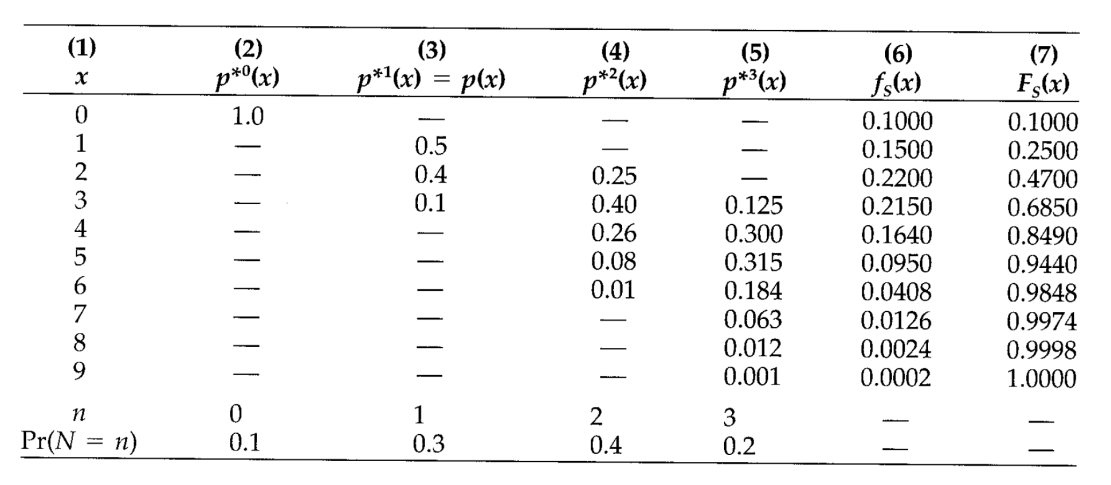
\includegraphics[width=0.75\linewidth]{Bowers Convolution 12.2.2 Example.png}
\end{figure}
\begin{itemize}
    \item The convolutions are done the usual way.
    \item The number of columns depend on the range of $N$.
    \item The $f_S(x)$ are the sumproduct of row $x$ and row $\Pr[N=n]$.
\end{itemize} \phantom{i}

\subsection{Distribution of $S$ in R}

\noi We will make extensive use of the function \texttt{aggregateDist} from the package \texttt{actuar} (Dutang, Goulet, and Pigeon 2008):
\begin{itemize}
  \item this function allows for several different aggregate distribution approaches, which will be introduced here (and in Module 4 as the associated theory is presented).
  \item here, we show how the function can be used to implement formulas (1) and (2) (using the function \texttt{convolve} in the background), which corresponds to the \texttt{method="convolution"} approach.
\end{itemize}

\noi The basic call is
\begin{lstlisting}
actuar::aggregateDist(method="convolution")
\end{lstlisting}
\noi with the following requirements and outputs:
\begin{itemize}
  \item A discrete distribution for \(Y\) is required.  Note that discretisation methods are discussed in Module 4.  This is input as a vector of claim‐amount probability masses via the argument \texttt{model.sev=}.  The first element must be \(\Pr[Y=0]\).
  \item There is no restriction on the shape of the frequency distribution, but it must have a finite range.  This is input as a vector of claim‐number probability masses via the argument \texttt{model.freq=}.  The first element must be \(\Pr[N=0]\).
  \item The outcome of the function is the df in (1).  Additional outputs:
    \begin{itemize}
      \item \texttt{plot}: to get a pretty plot of the df
      \item \texttt{summary}: to get summary statistics
      \item \texttt{mean}: to get the mean
      \item \texttt{diff}: to get the pmf
    \end{itemize}
  \item Additional options are:
    \begin{itemize}
      \item \texttt{x.scale}: currency units per unit of \texttt{sev} in the severity model (this allows calculations on multiples of \$1)
    \end{itemize}
\end{itemize}

\subsubsection{Example 12.2.2 (in R)}
\begin{lstlisting}
# Bowers 12.2.2
fy <- c(0, 0.5, 0.4, 0.1)
fn <- c(0.1, 0.3, 0.4, 0.2)
Fs <- aggregateDist("convolution", model.freq = fn, model.sev = fy)
mean(Fs)
## [1] 2.72
pmf <- c(Fs(0), diff(Fs(0:9)))
cbind(s = c(0:9), fs = pmf, Fs = Fs(0:9))
##      s   fs     Fs
## [1,] 0 0.1000 0.1000
## [2,] 1 0.1500 0.2500
## [3,] 2 0.2200 0.4700
## [4,] 3 0.2150 0.6850
## [5,] 4 0.1640 0.8490
## [6,] 5 0.0950 0.9440
## [7,] 6 0.0408 0.9848
## [8,] 7 0.0126 0.9974
## [9,] 8 0.0024 0.9998
## [10,] 9 0.0002 1.0000

summary(Fs)
## Aggregate Claim Amount Empirical CDF:
##  Min.   1st Qu.  Median  Mean 3rd Qu. Max.
## 0.00      2.00     3.00  2.72   4.00  9.00
plot(Fs)
\end{lstlisting}
\begin{figure}[H]
    \centering
    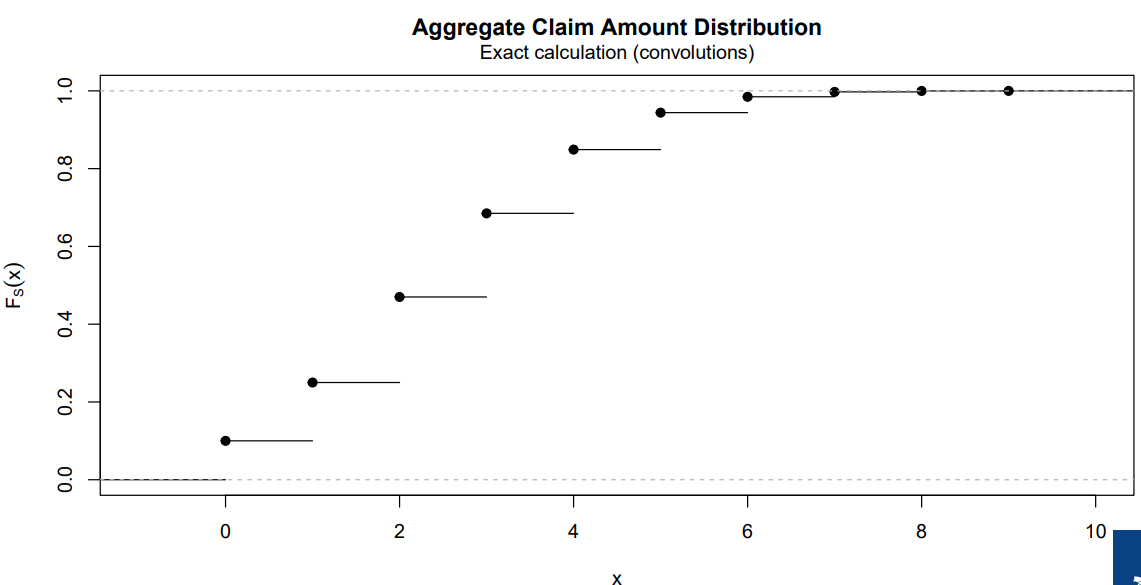
\includegraphics[width=0.75\linewidth]{Example 12.2.2 ECDF.png}
\end{figure}

\subsection{Basic models for claims frequency}

\noi in our case, we will assume that it directly affects the likelihood of a claim to occur, i.e., the frequency, such that \(N/\nu\) is normalised.

\noi MW defines
\[
p_k = \Pr[N = k], \quad k \in \mathcal{A} \subset \mathbb{N}_0,
\]
where \(\mathcal{A}\) is the set of possible frequency outcomes.

\noi there are three main assumptions for \(p_k\):
\begin{itemize}
  \item Binomial (with variance less than mean)
  \item Poisson (with variance equal to the mean)
  \item Negative binomial (a Poisson with random mean, so that variance is more than the mean)
\end{itemize}

\noi these all belong to a class of distributions called \((a,b)\), to be covered in Module 4

\subsubsection{Compound Binomial model}

\noi fixed volume \(\nu \in \mathbb{N}\)

\noi fixed default probability \(p \in (0,1)\) (expected claims frequency)

\noi pmf of \(N \sim \mathrm{Binom}(\nu,p)\) is
\[
p_k = \Pr[N = k]
= \binom{\nu}{k}\,p^k\,(1-p)^{\nu-k},
\quad k \in \{0,\dots,\nu\} = \mathcal{A}.
\]

\noi same as a sum of Bernoulli (which is the case \(\nu=1\))

\noi makes sense for a homogeneous portfolio with unique possible events, such as credit defaults or deaths in a life‐insurance model

\noi in R: \texttt{dbinom}, \texttt{pbinom}, \texttt{qbinom}, \texttt{rbinom}, where \texttt{size = \(\nu\)} and \texttt{prob = p}

\noi note that \(\binom{\nu}{k}\) can be computed with the R function \texttt{choose}

\noi The total claim amount \(S\) has a \textbf{compound Binomial distribution}
\[
S\sim\CompBinom(\nu,p,G)
\]
if \(N\sim\mathrm{Binom}(\nu,p)\) (with \(\nu\in\mathbb{N}\), \(p\in(0,1)\)) and individual claim‐size distribution \(G\).

\noi Corollary 2.7: Assume \(S_1,\dots,S_n\) are independent with
\[
S_j\sim\CompBinom(\nu_j,p,G),
\quad j=1,\dots,n.
\]
Then
\[
S=\sum_{j=1}^n S_j
\sim
\CompBinom\Bigl(\sum_{j=1}^n\nu_j,\;p,\;G\Bigr).
\]

\subsubsection{Compound Poisson model}

\noi fixed volume \(\nu > 0\)

\noi expected claims frequency \(\lambda > 0\)

\noi pmf of \(N \sim \Poi(\lambda\,\nu)\) is
\[
p_k = \Pr[N = k]
    = e^{-\lambda \nu}\,\frac{(\lambda \nu)^k}{k!},
    \quad k \in \mathcal{A} = \mathbb{N}_0.
\]

\noi Lemma 2.9: increasing volume \(\nu\) while keeping \(\mathbb{E}[N] = c = \nu p\) fixed in a Binomial model leads to a Poisson distribution (more so for small \(p\) compared to \(\nu\)):
\[
N_\nu \xrightarrow{d} N \sim \Poi(c)
\quad\text{for }N_\nu\sim\Binom(\nu,p),\ \lim_{\nu\to\infty}\nu p=c.
\]

\noi in R: \texttt{dpois}, \texttt{ppois}, \texttt{qpois}, \texttt{rpois}, where \(\lambda = \lambda\,\nu\)

\noi The total claim amount \(S\) has a \textbf{compound Poisson distribution}
\[
S \sim \CompPoi(\lambda\,\nu, G)
\]
if \(N\sim\Poi(\lambda\,\nu)\) for given \(\lambda,\nu>0\) and individual claim‐size distribution \(G\).

\noi the compound Poisson distribution has nice properties such as:
\begin{itemize}
  \item the aggregation property \(\uparrow\)
  \item the disjoint decomposition property \(\downarrow\)
\end{itemize}








\newpage
%%%%%%%%%%%%%%%%%%%%%%%%%%%%%%%%%%%%%%%%%%%%%%%%%%%%%%%%%%%%%%%%%%%%%%%%%%%%%%
\section{Module 3 – Individual Claim Size Modelling}

\subsection{Introduction}
\subsubsection{Steps in fitting loss models to data}
\noi
\begin{enumerate}
  \item \textbf{Explore and summarise data}
    \begin{itemize}
      \item graphical explorations
      \item empirical moments and quantiles
    \end{itemize}
  \item \textbf{Select a set of candidate distributions}
    \begin{itemize}
      \item Pareto, log-normal, inverse Gaussian, gamma, etc.
    \end{itemize}
  \item \textbf{Estimate the model parameters}
    \begin{itemize}
      \item method of moments
      \item maximum likelihood (MLE)
      \item maximum goodness (MGE)
    \end{itemize}
  \item \textbf{Evaluate the quality of a given model}
    \begin{itemize}
      \item graphical procedures (QQ, PP plots, empirical CDFs)
      \item score-based approaches (Kolmogorov–Smirnov tests, AD tests, chi-square goodness-of-fit tests)
      \item likelihood-based information criteria (AIC, BIC)
    \end{itemize}
  \item \textbf{Determine which model to choose based on needs}
\end{enumerate}

\subsubsection{Left‐truncation and right‐censoring}
\noi
\begin{itemize}
  \item \textbf{Left‐truncated observation} (e.g.\ excess / deductible) – exact value only recorded if it fulfils a certain condition:
    \begin{itemize}
      \item An observation is left‐truncated at \(c\) if it is \emph{not} recorded when it is at or below \(c\), and if it exceeds \(c\) it is recorded exactly.
    \end{itemize}
  \item \textbf{Right‐censored observation} (e.g.\ policy limit) – exact value not known:
    \begin{itemize}
      \item An observation is right‐censored at \(d\) if it is recorded as \(d\) when at or above \(d\), and if below \(d\) it is recorded exactly.
    \end{itemize}
  \item Similarly, one can define right‐truncation, left‐censoring, etc.
  \item Observations may be both left‐truncated and right‐censored, as often occurs in actuarial data.
\end{itemize}

\subsubsection{Zero claims}
\noi
\begin{itemize}
  \item Significant proportions of \textbf{zero claims} are frequent, for a number of reasons:
    \begin{itemize}
      \item data is policy‐based, not claims‐based;
      \item claims not exceeding deductible;
      \item mandatory reporting of accidents;
      \item “bonus hunger,” etc.
    \end{itemize}
  \item This complicates fitting, since many parametric severity distributions do not allow a flexible mass at 0.
  \item Several possible solutions:
    \begin{itemize}
      \item adjust \(Y\) by mixing in a point mass at 0 with a parametric distribution;
      \item adjust the claim frequency model (i.e.\ ignore zeros), but this
        \begin{itemize}
          \item may understate volatility (the proportion of zeros may itself be random),
          \item should be avoided if zeros represent claims of no cost (rather than absence of a claim).
        \end{itemize}
    \end{itemize}
\end{itemize}

\subsection{Data Analysis and Descriptive Statistics}
\begin{lstlisting}
# Using SUVA datasets from lectures
SUVA <- read_excel("SUVA.xls")
as_tibble(SUVA)
# This data set has 2 columns "medcosts" and "dailyallow"
\end{lstlisting}

\subsubsection{Preliminary Steps}
\noi Before any modelling is done, it is essential to gain a preliminary understanding of the data:
\begin{itemize}
  \item \textbf{Summarise the data}:
    \begin{itemize}
      \item summary statistics: mean, median, standard deviation, coefficient of variation, skewness, quantiles, min, max, etc.
    \end{itemize}
  \item \textbf{Visualise the data}:
    \begin{itemize}
      \item histogram with kernel density overlay,
      \item empirical CDF, compared to a theoretical CDF via QQ or PP plot.
    \end{itemize}
  \item For heavy‐tailed data, repeat the above on the log‐scale (e.g.\ compare to lognormal).
  \item Understand data collection procedures and standards.
  \item Investigate any unusual features (outliers, breaks, etc.\ ) by consulting claim adjusters or data owners if possible.
\end{itemize}

\subsubsection{Visualise the SUVA raw data}
\begin{lstlisting}
fitdistrplus::plotdist(SUVA$medcosts, histo = TRUE, demp = TRUE)
sum(SUVA$medcosts > 0)/length(SUVA$medcosts)
## [1] 0.966896
\end{lstlisting}
\begin{figure}[H]
    \centering
    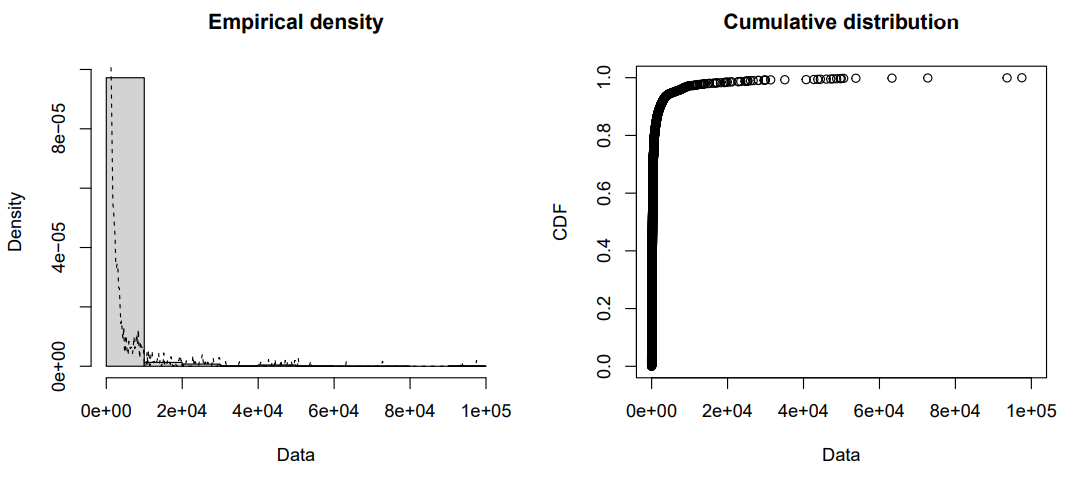
\includegraphics[width=0.7\linewidth]{SUVA - medcosts - plot.png}
\end{figure}

\subsubsection*{Log of raw SUVA data}
\begin{lstlisting}
fitdistrplus::plotdist(log(SUVA$medcosts[SUVA$medcosts > 0]), histo = TRUE,
demp = TRUE)
\end{lstlisting}
\begin{figure}[H]
    \centering
    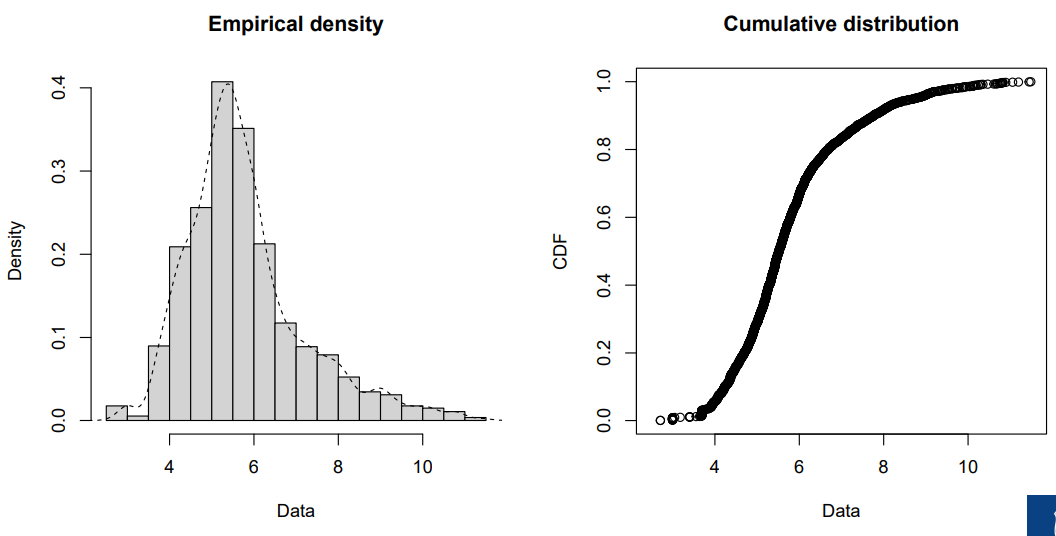
\includegraphics[width=0.7\linewidth]{SUVA data - log plot.png}
\end{figure}

\begin{itemize}
  \item Medical costs remain skewed even on the log scale, suggesting an extremely heavy‐tailed distribution may be necessary.
  \item Daily allowance costs look roughly symmetric after logging, suggesting a lognormal (or similar) model might be appropriate.
  \item Removing zeros is crucial for the daily allowance data (and for taking logarithms), since more than half of the claims are zero.
\end{itemize}

\subsubsection{Moments}
\noi Moments of a distribution provide information:
\begin{itemize}
  \item The first moment is the mean, which provides its location.
  \item The second \emph{central} moment is the variance (and is related to the coefficient of variation), giving an idea of dispersion around the mean.
  \item The third \emph{standardized} moment is the skewness of the data.
  \item The fourth \emph{standardized} moment is the kurtosis, which indicates tail‐fatness.
    \begin{itemize}
      \item Excess kurtosis $=$ kurtosis $-3$, measured relative to the normal distribution.
    \end{itemize}
\end{itemize}

\subsubsection*{Loss size index and mean excess function}
\noi The following summary functions are also helpful:
\begin{itemize}
  \item \textbf{Loss‐size index function} of \(y\):
    \[
      \mathcal I\bigl(G(y)\bigr)
      = \frac{\displaystyle\int_{0}^{y} z\,\mathrm{d}G(z)}
             {\displaystyle\int_{0}^{\infty} z\,\mathrm{d}G(z)},
      \quad
      \widehat{\mathcal I}_n(\alpha)
      = \frac{\sum_{i=1}^{\lfloor n\alpha\rfloor}Y_{(i)}}
             {\sum_{i=1}^{n}Y_i},
      \quad \alpha\in[0,1].
    \]
    This measures the contribution of \([0,y]\) to the overall mean (cf.\ Pareto principle: 80\% of cost from top 20\% of claims).
  \item \textbf{Mean excess function} of \(u\):
    \[
      e(u) = E\bigl[Y - u \mid Y>u\bigr],
      \quad
      \widehat e_n(u)
      = \frac{\sum_{i=1}^n (Y_i - u)\,1_{\{Y_i>u\}}}
             {\sum_{i=1}^n 1_{\{Y_i>u\}}}.
    \]
    An increasing \(e(u)\) indicates a heavy‐tailed distribution (see Module 6).  Note \(e(0)\) is the mean when all claims are strictly positive.
\end{itemize} \phantom{i}

\noi \textbf{R and Technical Notes}: \\
\begin{itemize}
  \item To compute empirical quantities:
    \begin{itemize}
      \item \texttt{actuar::emm} provides empirical moments of any order.
      \item \texttt{mean}, \texttt{var}, \texttt{sd} give the (unbiased) sample mean, variance, and standard deviation.
      \item Code for the loss‐size index function is provided in the illustration.
      \item Code for the mean‐excess function is also provided, though one often uses \texttt{extRemes::mrlplot()} for plotting.
    \end{itemize}
  \item The function \texttt{fitdistrplus::descdist()} produces a skewness–kurtosis plot showing the empirical point relative to the theoretical region for various distributions.
    \begin{itemize}
      \item The \texttt{boot} parameter enables non‐parametric bootstrap of the moment estimates to assess variability.
      \item The \texttt{method} argument may be \texttt{"unbiased"} or \texttt{"sample"} to switch between unbiased or sample moments.
    \end{itemize}
\end{itemize}

\subsubsection{SUVA Moments}
\noi \textbf{Medical Costs}:
\begin{lstlisting}
format(actuar::emm(SUVA$medcosts, order = 1:3), scientific = FALSE)
## [1] " 1443.349" " 34268506.007" "1791560934502.502"
sd(SUVA$medcosts)/mean(SUVA$medcosts)
## [1] 3.93143
\end{lstlisting}

\noi \textbf{Daily Allowance}:
\begin{lstlisting}
format(actuar::emm(SUVA$dailyallow, order = 1:3), scientific = FALSE)
## [1] " 3194.15" " 172677852.63" "20364647975482.07"
sd(SUVA$dailyallow)/mean(SUVA$dailyallow)
## [1] 3.991459
\end{lstlisting}

\subsubsection{Skewness and Kurtosis Plots (Cullen and Frey)}
\begin{lstlisting}
fitdistrplus::descdist(log(SUVA$medcosts[SUVA$medcosts > 0]), boot = 1000)
\end{lstlisting}
\begin{figure}[H]
    \centering
    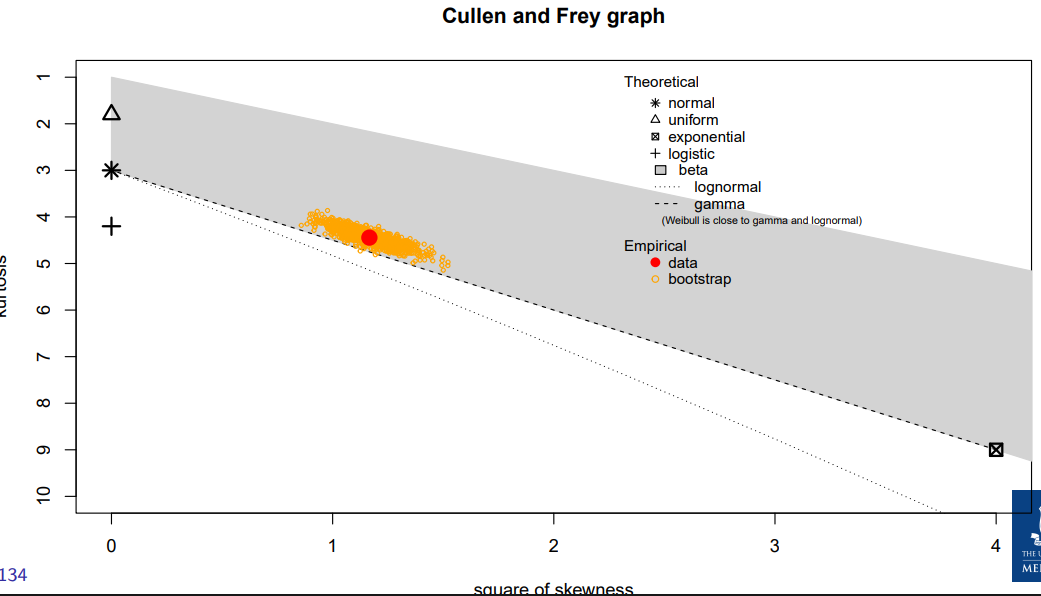
\includegraphics[width=0.7\linewidth]{SUVA data - Cullen and Frey - MedCosts.png}
\end{figure}

\begin{lstlisting}
fitdistrplus::descdist(log(SUVA$dailyallow[SUVA$medcosts > 0]), boot = 1000)
## summary statistics
## ------
## min: 3.258097 max: 12.13806
## median: 7.474772
## mean: 7.63051
## estimated sd: 1.441014
## estimated skewness: 0.3378648
## estimated kurtosis: 3.259708
\end{lstlisting}
\begin{figure}[H]
    \centering
    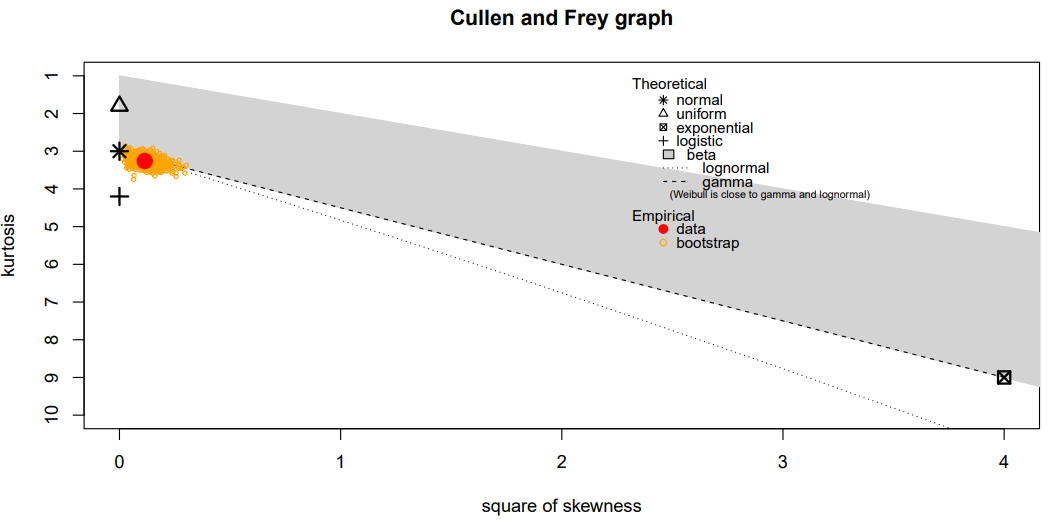
\includegraphics[width=0.7\linewidth]{SUVA data - Cullen and Frey - Daily Allow.png}
\end{figure}

\subsubsection{Loss Index Function}
\begin{lstlisting}
SUVA.MC.lif <- cumsum(sort(SUVA$medcosts))/sum(SUVA$medcosts)
plot(1:length(SUVA$medcosts)/length(SUVA$medcosts),
    SUVA.MC.lif, xlab = "number of claims (in 100%)",
    ylab = "empirical loss size index function")
abline(h = 0.2, v = 0.8)
\end{lstlisting}
\begin{figure}[H]
    \centering
    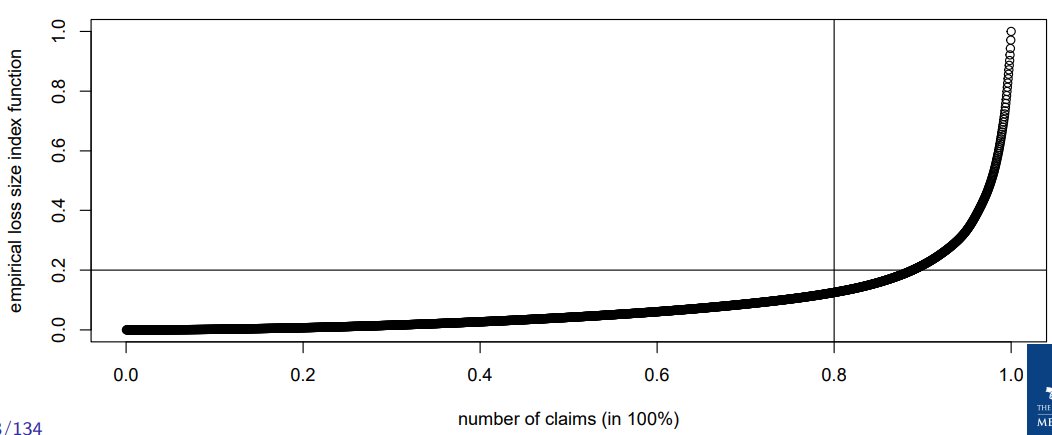
\includegraphics[width=0.7\linewidth]{SUVA - Loss Index Function - Med Costs.png}
\end{figure}

\begin{lstlisting}
SUVA.DA.lif <- cumsum(sort(SUVA$dailyallow))/sum(SUVA$dailyallow)
plot(1:length(SUVA$dailyallow)/length(SUVA$dailyallow),
    SUVA.DA.lif, xlab = "number of claims (in 100%)",
    ylab = "empirical loss size index function")
abline(h = 0.2, v = 0.8)
\end{lstlisting}
\begin{figure}[H]
    \centering
    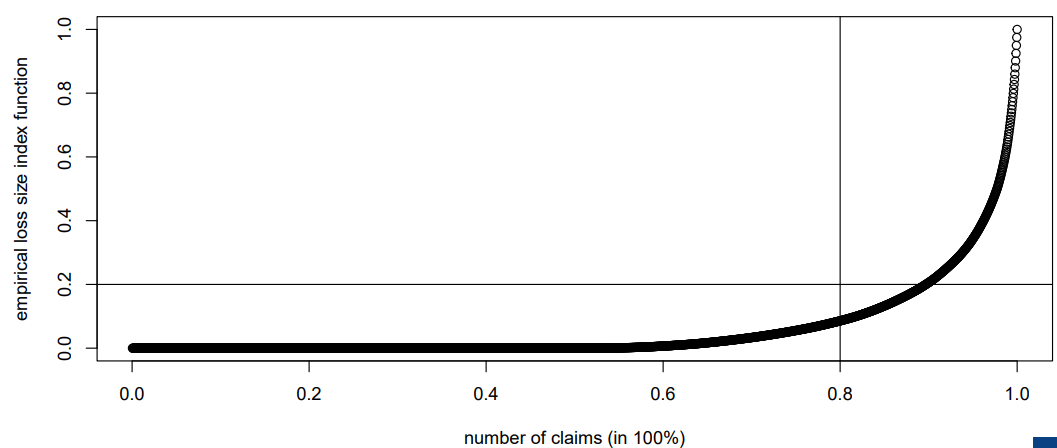
\includegraphics[width=0.7\linewidth]{SUVA - Loss Index Function - Daily Allow.png}
\end{figure}

\subsubsection{Mean-Excess Plot}
\noi This function will return the mean excess function for an arbitrary vector of
thresholds $u$ (for instance, 0, 100, 1000 and 10000 here)
\begin{lstlisting}
mef <- function(x, u) {
mefvector <- c()
for (i in u) {
mefvector <- c(mefvector, sum(pmax(sort(x) - i, 0))/length(x[x >
i]))
}
return(mefvector)
}
mef(SUVA$medcosts, c(0, 100, 1000, 10000))
## [1] 1492.765 1709.148 6233.296 18156.631
mean(SUVA$medcosts)
## [1] 1443.349
mean(SUVA$medcosts[SUVA$medcosts > 0])
## [1] 1492.765
\end{lstlisting}

\noi This graph is done easily using \texttt{extRemes::mrlplot} (a linear increase means its heavy tailed):
\begin{lstlisting}
mrlplot(SUVA$medcosts[SUVA$medcosts > 0], xlim = c(250, 20000))
# If you restrict the x range the graph isn't biased by a few very large values
\end{lstlisting}
\begin{figure}[H]
    \centering
    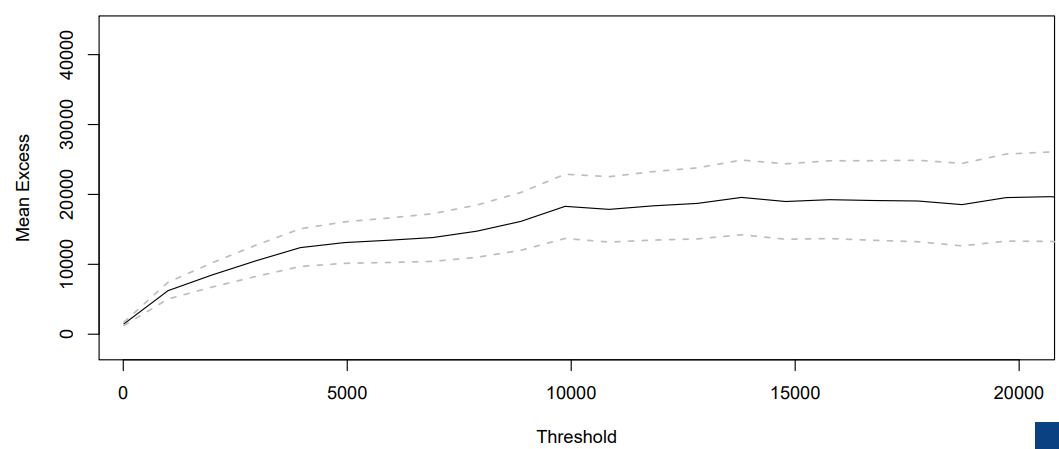
\includegraphics[width=0.7\linewidth]{SUVA - MRL - MedCosts.png}
\end{figure}

\begin{lstlisting}
mrlplot(SUVA$dailyallow[SUVA$dailyallow > 0], xlim = c(250, 1e+05))
# again restrict xlim, because it shows its not as heavy tail as the whole domain says
# its kind of flat
\end{lstlisting}
\begin{figure}[H]
    \centering
    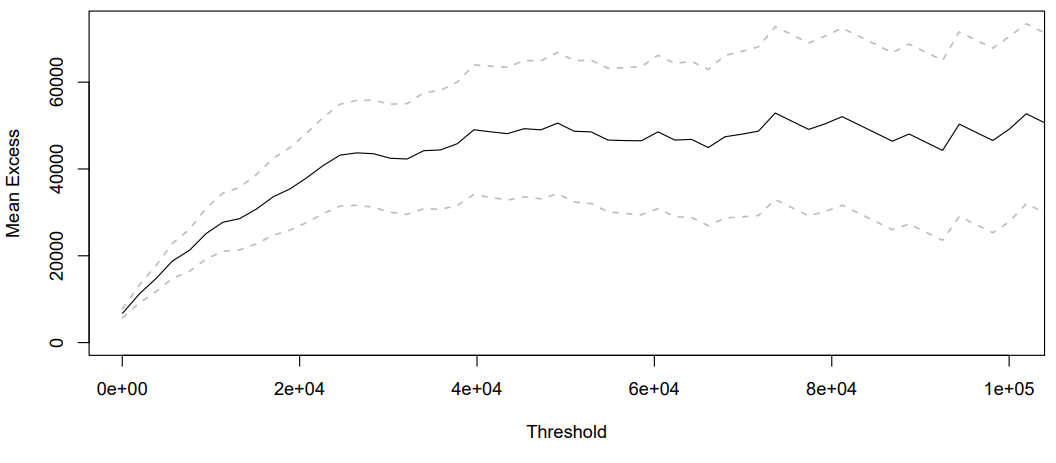
\includegraphics[width=0.7\linewidth]{SUVA - MRL - Daily Allow.png}
\end{figure}

\subsubsection{Quantiles}
\begin{lstlisting}
quantile(SUVA$dailyallow[SUVA$dailyallow > 0])
##   0%   25%    50%    75%     100%
## 26.0 842.0 1763.0 4841.5 186850.0

#### could also focus on particular quantiles
quantile(SUVA$medcosts[SUVA$medcosts > 0], probs = c(0.9, 0.95, 0.97, 0.99))
##     90%     95%     97%      99%
## 2351.00 6120.20 9661.08 27450.60
quantile(SUVA$dailyallow[SUVA$dailyallow > 0], probs = c(0.9, 0.95, 0.97, 0.99))
##     90%     95%     97%     99%
## 14015.0 25140.5 41896.7 93285.0
\end{lstlisting}
\noi This is a crude way of estimating Value at Risk (VaR)

\subsubsection{Boxplots}
\begin{lstlisting}
boxplot(list(`Medical costs` = log(SUVA$medcosts[SUVA$medcosts > 0]),
`Daily allowance` = log(SUVA$dailyallow[SUVA$dailyallow > 0])))
# the unlogged version is too bad to see anything
\end{lstlisting}
\begin{figure}[H]
    \centering
    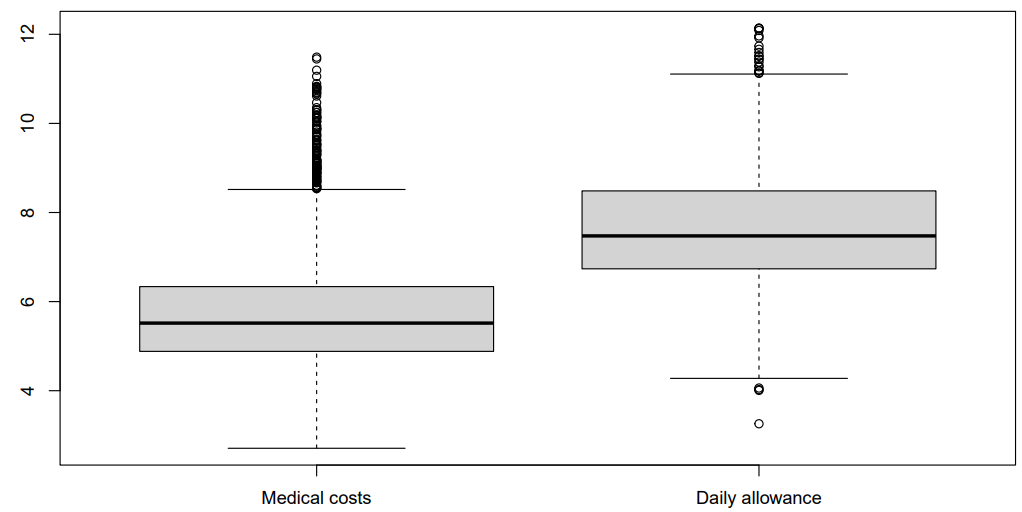
\includegraphics[width=0.7\linewidth]{SUVA - Box Plots.png}
\end{figure}

\subsubsection{Log-Log Plots}
\noi The log‐log plot is defined as
\[
y\;\mapsto\;\bigl[\ln y,\;\ln\bigl(1 - G(y)\bigr)\bigr],
\]
where \(G\) is replaced by \(\widehat G\) in the empirical version.  Just as for the empirical mean‐excess plot, a linear (now decreasing) pattern in the empirical log‐log plot suggests a heavy‐tailed distribution.

\begin{lstlisting}
emplot(SUVA$medcosts[SUVA$medcosts > 0], alog = "xy", labels = TRUE)
\end{lstlisting}
\begin{figure}[H]
    \centering
    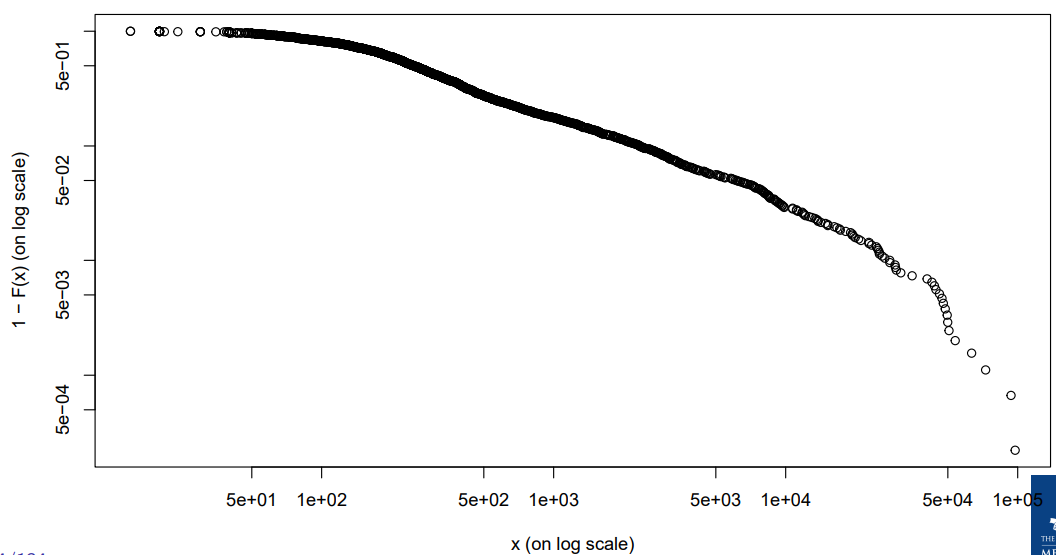
\includegraphics[width=0.7\linewidth]{SUVA - Log-Log - MedCosts.png}
\end{figure}

\begin{lstlisting}
emplot(SUVA$dailyallow[SUVA$dailyallow > 0], alog = "xy", labels = TRUE)
\end{lstlisting}
\begin{figure}[H]
    \centering
    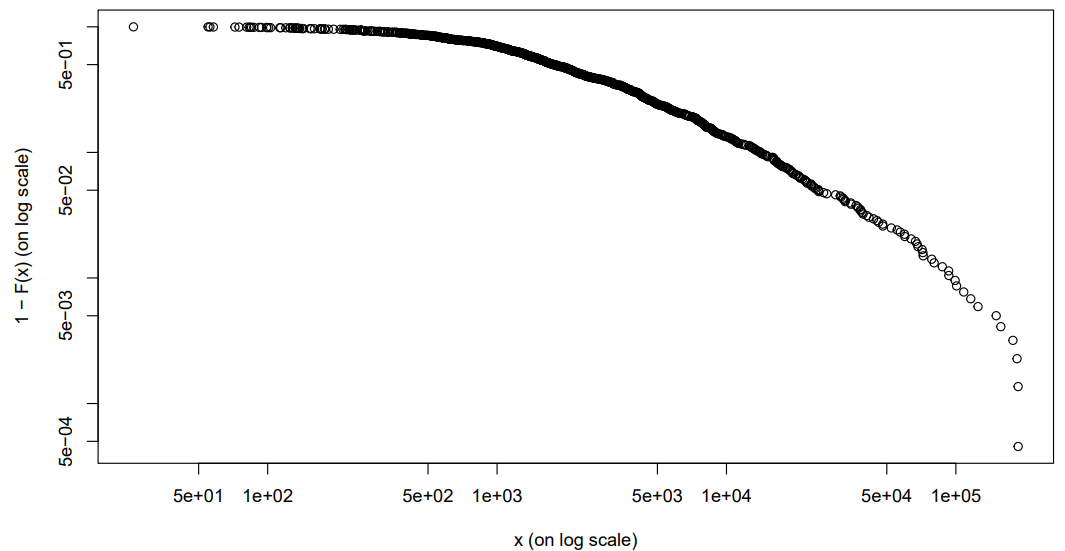
\includegraphics[width=0.7\linewidth]{SUVA - Log-Log - Daily Allow.png}
\end{figure}

\noi Again, medical costs are a good candidate for heavy tailed distributions
(graph is more linear, except at the very end), whereas daily allowance is
more reasonably behaved (graph is more concave).

\subsection{Parametric Models (Distributions) for Severity}
\subsubsection{Gamma distribution}
\noi Let \(Y\sim\Gamma(\alpha,\beta)\) with density
\[
g(y)=\frac{\beta^\alpha}{\Gamma(\alpha)}\,y^{\alpha-1}e^{-\beta y}, 
\quad y>0,\ \alpha,\beta>0.
\]
\begin{itemize}
  \item \textbf{CDF}: 
  \[
    G(y)=\frac{1}{\Gamma(\alpha)}\int_{0}^{\beta y}t^{\alpha-1}e^{-t}\,dt
    =P\bigl(\alpha,\beta y\bigr),
  \]
  where \(P\) is the regularized lower incomplete gamma.
  \item \textbf{Mean}: \(\E[Y]=\alpha/\beta\).
  \item \textbf{Variance}: \(\Var(Y)=\alpha/\beta^2\).
  \item \textbf{Skewness}: \(\gamma_1(Y)=2/\sqrt{\alpha}.\)
  \item \textbf{MGF}: \(M_Y(t)=\bigl(\tfrac{\beta}{\beta-t}\bigr)^{\alpha},\ t<\beta.\)
  \item \textbf{Moments}: \(\E[Y^k]=\Gamma(\alpha+k)\,/\,\bigl(\Gamma(\alpha)\,\beta^k\bigr).\)
  \item \textbf{Special case}: \(\alpha=1\implies Y\sim\Exp(\beta).\)
\end{itemize}

\subsubsection{Inverse Gaussian distribution}
\noi Let \(Y\sim\IG(\alpha,\beta)\) with density
\[
g(y)
=\frac{\alpha\,y^{-3/2}}{\sqrt{2\pi\beta}}
\exp\!\Bigl[-\frac{(\alpha-\beta y)^2}{2\beta y}\Bigr],
\quad y>0,\ \alpha,\beta>0.
\]
\begin{itemize}
  \item \textbf{Mean}: \(\E[Y]=\alpha/\beta\).
  \item \textbf{Variance}: \(\Var(Y)=\alpha/\beta^2\).
  \item \textbf{Skewness}: \(\gamma_1(Y)=3/\sqrt{\alpha}.\)
  \item \textbf{MGF}: \(M_Y(t)=\exp\!\bigl[\alpha\,(1-\sqrt{1-2t/\beta})\bigr],\ t<\beta/2.\)
  \item \textbf{CDF}: no simple closed form; expressible via standard normal CDFs.
\end{itemize}

\subsubsection{Weibull distribution}
\noi Let \(Y\sim\Weibull(\tau,c)\) with density
\[
g(y)=(c\,\tau)\,(c\,y)^{\tau-1}e^{-(c\,y)^\tau},
\quad y>0,\ c,\tau>0.
\]
\begin{itemize}
  \item \textbf{CDF}: \(G(y)=1-\exp\{-(c\,y)^\tau\}.\)
  \item \textbf{Mean}: \(\E[Y]=\Gamma(1+1/\tau)/c.\)
  \item \textbf{Variance}: \(\Var(Y)=\Gamma(1+2/\tau)/c^2 -\mu_Y^2.\)
  \item \textbf{Skewness}: 
    \(\gamma_1(Y)
    =\bigl[\Gamma(1+3/\tau)/c^3 -3\mu_Y\sigma_Y^2-\mu_Y^3\bigr]/\sigma_Y^3.\)
  \item \textbf{MGF}: does not exist for \(\tau<1\) and \(t>0\).
  \item \textbf{Moments}: \(\E[Y^k]=\Gamma(1+k/\tau)/c^k.\)
  \item \textbf{Note}: If \(Z\sim\Exp(1)\), then \(Z^{1/\tau}/c\sim\Weibull(\tau,c)\).
\end{itemize}

\subsubsection{Lognormal distribution}
\noi Let \(Y\sim\LN(\mu,\sigma^2)\), so \(\ln Y\sim\N(\mu,\sigma^2)\).
\begin{itemize}
  \item \textbf{CDF}: \(\Pr(Y\le y)=\Phi\bigl((\ln y-\mu)/\sigma\bigr).\)
  \item \textbf{Mean}: \(\E[Y]=\exp\{\mu+\sigma^2/2\}.\)
  \item \textbf{Variance}: \(\Var(Y)=\exp\{2\mu+\sigma^2\}\bigl(\exp\{\sigma^2\}-1\bigr).\)
  \item \textbf{Skewness}: \((\exp\{\sigma^2\}+2)\sqrt{\exp\{\sigma^2\}-1}.\)
  \item \textbf{MGF}: does not exist for \(t>0\).
\end{itemize}

\subsubsection{Log‐gamma distribution}
\noi If \(\ln Y\sim\Gamma(\gamma,c)\), then \(Y\) has density
\[
g(y)=\frac{c^\gamma}{\Gamma(\gamma)}(\ln y)^{\gamma-1}y^{-(c+1)},
\quad y>0,\ \gamma,c>0.
\]
\begin{itemize}
  \item \textbf{CDF}: 
  \(\displaystyle
    G(y)
    =\frac{1}{\Gamma(\gamma)}
     \int_{0}^{\ln y} t^{\gamma-1}e^{-c\,t}\,dt\).
  \item \textbf{Mean}: \(\E[Y]=(c/(c-1))^\gamma\), \(c>1\).
  \item \textbf{Variance}: \(\Var(Y)=(c/(c-2))^\gamma -\mu_Y^2\), \(c>2\).
  \item \textbf{Skewness}: 
    \(\bigl[(c/(c-3))^\gamma -3\mu_Y\sigma_Y^2-\mu_Y^3\bigr]/\sigma_Y^3\), \(c>3\).
  \item \textbf{MGF}: does not exist for \(t>0\).
  \item \textbf{Moments}: \(\E[Y^k]=(c/(c-k))^\gamma,\;c>k.\)
\end{itemize}

\subsubsection{Pareto distribution}
\noi Let \(Y\sim\Pareto(\theta,\alpha)\) with density
\[
g(y)=\frac{\alpha}{\theta}\Bigl(\frac{y}{\theta}\Bigr)^{-(\alpha+1)},
\quad y\ge\theta,\ \alpha>0.
\]
\begin{itemize}
  \item \textbf{CDF}: \(G(y)=1-\bigl(\theta/y\bigr)^{\alpha},\ y\ge\theta.\)
  \item \textbf{Mean}: \(\E[Y]=\theta\,\alpha/(\alpha-1),\ \alpha>1.\)
  \item \textbf{Variance}: \(\Var(Y)=\theta^2\,\frac{\alpha}{(\alpha-1)^2(\alpha-2)},\ \alpha>2.\)
  \item \textbf{Skewness}: 
    \(\gamma_1(Y)
    =\frac{2(1+\alpha)/(\alpha-3)\,\sqrt{(\alpha-2)/\alpha}}{\,},\ \alpha>3.\)
  \item \textbf{MGF}: does not exist for \(t>0\).
\end{itemize}

\subsection{Modelling Zero Claims}
\subsubsection{Zero‐inflated severity model \(X = I\,B\)}
\noi In this approach \(X=I\,B\), where
\begin{itemize}
  \item \(I\) is an indicator of whether a claim occurs, with
    \[
      \Pr[I=1]=q,\qquad \Pr[I=0]=1-q.
    \]
  \item \(B\) is the claim amount given \(I=1\).
\end{itemize}

\subsubsection*{Resulting distribution}
\[
\Pr[X \le x]
= \Pr[X \le x \mid I=0]\Pr[I=0]
  + \Pr[X \le x \mid I=1]\Pr[I=1]
= (1-q) + q\,\Pr[B \le x].
\]
Hence the moment generating function is
\[
M_X(t)
= \mathbb{E}[e^{tX}]
= \mathbb{E}[e^{tX}\mid I=0]\,(1-q) + \mathbb{E}[e^{tX}\mid I=1]\,q
= (1-q) + q\,\mathbb{E}[e^{tB}].
\]

\subsubsection*{Mean and Variance}
\noi By conditioning,
\[
\mathbb{E}[X]
= \mathbb{E}\bigl[\mathbb{E}[X\mid I]\bigr]
= \mathbb{E}\bigl[I\;\mathbb{E}[B]\bigr]
= q\,\mathbb{E}[B],
\]
and
\[
\text{Var}(X)
= \text{Var}\bigl(\mathbb{E}[X\mid I]\bigr)
  + \mathbb{E}\bigl[\text{Var}(X\mid I)\bigr]
= (\mathbb{E}[B])^2\,\text{Var}(I)
  + \mathbb{E}[I^2]\,\text{Var}(B)
= q(1-q)\,(\mathbb{E}[B])^2 + q\,\text{Var}(B).
\]

\subsubsection*{Special case: \(X = I\,b\)}
\begin{itemize}
  \item Fixed claim amount \(B=b\) w.p.\ 1.
  \item Then \(X=I\,b\) takes
    \[
      X = 
      \begin{cases}
        b, & I=1,\\
        0, & I=0,
      \end{cases}
    \]
    so \(\mathbb{E}[X]=b\,q\) and \(\text{Var}(X)=b^2\,q(1-q)\).  In other words, \(X\) is a scaled Bernoulli\@.
\end{itemize}

\subsubsection*{Example: Bicycle Theft (retrieving \(B\) from \(X\))}
\noi An insurer covers bicycle theft up to \(\$400\), but pays only half if the bike was not locked.  Suppose
\[
\Pr[X=400]=0.05,\quad \Pr[X=200]=0.15,
\quad q=\Pr[I=1]=0.20.
\]
Then for \(x=400\) we back out
\[
\Pr[B=400]
= \Pr[X=400 \mid I=1]
= \frac{\Pr[X=400\;\cap\;I=1]}{\Pr[I=1]}
= \frac{0.05}{0.20}
= 0.25.
\]

\subsection{Fitting of Distributions}
\noi Some fitting criteria include:
\begin{itemize}
    \item moment matching: choose the m parameters such that the first $m$ moments match
    \item maximum likelihood: choose the parameters such that the overall likelihood that the model generated the data is maximal
\end{itemize} \phantom{i}

\noi \textbf{R and Technical Notes}:
\begin{itemize}
    \item \texttt{MASS::fitdist} is standard, and uses by default MLE via the \texttt{optim} function.
    \item \texttt{fitdistrplus} allows other fitting criteria (such as method of moments and maximum goodness), and also allows for the user to supply their own optimisation function.
    \item distributions are coded in the following way, e.g., for distribution \texttt{foo}:
        \begin{itemize}
            \item \texttt{dfoo} is the density (pdf)
            \item \texttt{pfoo} is the distribution function (cdf)
            \item \texttt{qfoo} is the quantile function
            \item \texttt{rfoo} is the random number generator
        \end{itemize}
\end{itemize}

\subsubsection{Moment Matching Estimation (Theory and R Example)}
\noi This is quite straightforward—for a distribution with \(m\) parameters:
\begin{itemize}
  \item Choose \(m\) moments you care about (usually the first \(m\) moments about the origin or the mean).
  \item Build a system of \(m\) equations (one per parameter) equating the theoretical moments to the empirical moments.
  \item Solve the system (analytically if possible, otherwise numerically).
\end{itemize}

\noi In R, set the argument \texttt{method="mme"} in the call to \texttt{fitdist}:
\begin{itemize}
  \item For 1‐ and 2‐parameter distributions, the mean and variance are matched in closed form.
  \item For some other distributions, closed‐form solutions for higher moments are used.
  \item Otherwise, the equations are solved numerically (via \texttt{optim}), minimising the sum of squared differences between theoretical and empirical moments.
\end{itemize}

\subsubsection*{R SUVA Data Example}
\begin{lstlisting}
fit.lnorm.mme <- fitdistrplus::fitdist(log(SUVA$dailyallow[SUVA$dailyallow 0]),
    "lnorm", method = "mme", order = 1:2)
fit.lnorm.mme$estimate
##   meanlog     sdlog
## 2.0146490 0.1871132

fit.lnorm.mme$loglik
## [1] -1959.06

fit.gamma.mme <- fitdist(log(SUVA$dailyallow[SUVA$dailyallow > 0]),
    "gamma", method = "mme", order = 1:2)
fit.gamma.mme$estimate
##     shape     rate
## 28.065081 3.678009

fit.gamma.mme$loglik
## [1] -1951.838

# function to calculate sample raw moment
memp <- function(x, order) emm(x, order)
fit.weibull.mme <- fitdist(log(SUVA$dailyallow[SUVA$dailyallow > 0]),
    "weibull", method = "mme", memp = memp, order = c(1, 2))
fit.weibull.mme$estimate
##    shape    scale
## 6.172910 8.212158

fit.weibull.mme$loglik
## [1] -2020.119
\end{lstlisting}

\subsubsection{Maximum Likelihood Estimation (Theory and R Example)}
\noi The likelihood for a statistical model indicates how probable the observed data are under the model.  Without censoring or truncation, for observations \(\mathbf{x}=(x_1,\dots,x_n)\) and parameter vector \(\theta=(\theta_1,\dots,\theta_m)\),
\[
L(\theta;\mathbf{x})
= \prod_{i=1}^n f(x_i;\theta).
\]
The value \(\widehat\theta\) that maximizes \(L(\theta;\mathbf{x})\) is the \emph{maximum likelihood estimator}.  It is more convenient to maximize the log-likelihood
\[
\ell(\theta;\mathbf{x})
= \log L(\theta;\mathbf{x}),
\]
which avoids numerical underflow when \(n\) is large.  MLEs enjoy properties such as consistency and asymptotic normality, allowing standard errors to be estimated via the observed information matrix.

\subsubsection*{R SUVA Data Example}
\begin{lstlisting}
fit.lnorm.mle <- fitdist(log(SUVA$dailyallow[SUVA$dailyallow > 0]),
    "lnorm", method = "mle")
fit.lnorm.mle$estimate
##   meanlog     sdlog
## 2.0140792 0.1918442

fit.lnorm.mle$loglik
## [1] -1958.359

fit.gamma.mle <- fitdist(log(SUVA$dailyallow[SUVA$dailyallow > 0]),
    "gamma")
fit.gamma.mle$estimate
##     shape     rate
## 27.819839 3.646072

fit.gamma.mle$loglik
## [1] -1951.818

fit.weibull.mle <- fitdist(log(SUVA$dailyallow[SUVA$dailyallow > 0]),
    "weibull")
fit.weibull.mle$estimate
##   shape     scale
## 5.527347 8.231313

fit.weibull.mle$loglik
## [1] -2003.26

summary(fit.weibull.mle)
## Fitting of the distribution ' weibull ' by maximum likelihood
## Parameters :
##       estimate Std. Error
## shape 5.527347 0.12127037
## scale 8.231313 0.04760155
## Loglikelihood: -2003.26 AIC: 4010.519 BIC: 4020.524
## Correlation matrix:
##           shape     scale
## shape 1.0000000 0.3301744
## scale 0.3301744 1.0000000
\end{lstlisting}

\subsection{Parameter Uncertainty}
\subsubsection{Hessian matrix}
\noi The \emph{score} (or gradient) vector consists of the first derivatives of the log‐likelihood \(\ell(\theta;\mathbf{x})\):
\[
S(\theta;\mathbf{x})
=\begin{pmatrix}
\displaystyle\frac{\partial\ell(\theta;\mathbf{x})}{\partial\theta_1},\;\dots,\;
\displaystyle\frac{\partial\ell(\theta;\mathbf{x})}{\partial\theta_m}
\end{pmatrix}^{\!\prime},
\]
so that the MLE \(\widehat\theta\) satisfies the first‐order condition
\[
S(\widehat\theta;\mathbf{x}) \;=\; \mathbf{0}.
\]
The \(m\times m\) \emph{Hessian} matrix is the matrix of second derivatives:
\[
H(\theta;\mathbf{x})
=\frac{\partial^2\ell(\theta;\mathbf{x})}
      {\partial\theta\,\partial\theta^{\prime}}
=\begin{pmatrix}
\displaystyle\frac{\partial^2\ell(\theta;\mathbf{x})}
                  {\partial\theta_1^2} & \dots &
\displaystyle\frac{\partial^2\ell(\theta;\mathbf{x})}
                  {\partial\theta_1\,\partial\theta_m}
\\[1ex]
\vdots & \ddots & \vdots
\\[1ex]
\displaystyle\frac{\partial^2\ell(\theta;\mathbf{x})}
                  {\partial\theta_m\,\partial\theta_1}
& \dots &
\displaystyle\frac{\partial^2\ell(\theta;\mathbf{x})}
                  {\partial\theta_m^2}
\end{pmatrix}.
\]
The \emph{Fisher information} is the (expected) variance of the score:
\[
\mathcal{I}(\theta)
=-\,\mathbb{E}\bigl[\,H(\theta;\mathbf{x})\bigr].
\]

\subsubsection{The Wald approximation}
\noi A consistent estimator of the covariance matrix of \(\widehat\theta\) is given by the inverse of the estimated Fisher information at \(\widehat\theta\):
\[
\text{Var}(\widehat\theta)
\;\approx\;
\bigl[-\,\mathbb{E}\bigl(H(\widehat\theta;\mathbf{x})\bigr)\bigr]^{-1}.
\]
The square roots of the diagonal entries of this matrix are the standard errors of the MLE.  Here:
\begin{itemize}
  \item “Consistent” means convergence in probability to the true value.
  \item As \(n\to\infty\), \(\widehat\theta\) is asymptotically normal.
  \item These are asymptotic results, and in practice depend on the data, the model, and the parametrisation.
\end{itemize}

\subsubsection{Standard errors for SUVA data}
\begin{lstlisting}
# You can't get this for MME, only MLE:
fit.lnorm.mle$sd
##     meanlog       sdlog
## 0.005786951 0.004091492

fit.gamma.mle$sd
##     shape      rate
## 1.1797330 0.1560157

fit.weibull.mle$sd
##      shape      scale
## 0.12127037 0.04760155
\end{lstlisting}

\subsection{Dealing with left-truncation and right-censoring}
\subsubsection{Likelihood with left‐truncation and right‐censoring}

\noindent Suppose we observe triplets \((t_j,x_j,\delta_j)\), \(j=1,\dots,n\), where
\begin{itemize}
  \item \(t_j\) is the left‐truncation threshold (data are only recorded if \(X>t_j\)),
  \item \(x_j\) is the recorded value (either the exact loss or the censoring limit),
  \item \(\delta_j\) is the right‐censoring indicator:
    \[
      \delta_j=\begin{cases}
        0,&\text{if the observation is exact (limit not reached),}\\
        1,&\text{if right‐censored (limit reached).}
      \end{cases}
    \]
\end{itemize}
\noindent If the underlying model has pdf \(f(\,\cdot\,;\theta)\) and cdf \(F(\,\cdot\,;\theta)\), then the contribution of observation \(j\) to the likelihood is
\[
L_j(\theta)
=\biggl[\frac{f(x_j;\theta)}{1 - F(t_j;\theta)}\biggr]^{1-\delta_j}
\;\times\;
\biggl[\frac{1 - F(x_j;\theta)}{1 - F(t_j;\theta)}\biggr]^{\delta_j}.
\]
Hence the full likelihood is
\[
L(\theta)
=\prod_{j=1}^n
\biggl[\frac{f(x_j;\theta)}{1 - F(t_j;\theta)}\biggr]^{1-\delta_j}
\;\times\;
\biggl[\frac{1 - F(x_j;\theta)}{1 - F(t_j;\theta)}\biggr]^{\delta_j}.
\]
\noindent Equivalently:
\begin{itemize}
  \item If \(\delta_j=0\) (exact), \(L_j(\theta)=f(x_j;\theta)/(1-F(t_j;\theta))\).
  \item If \(\delta_j=1\) (censored), \(L_j(\theta)=[1-F(x_j;\theta)]/(1-F(t_j;\theta))\).
\end{itemize}
\noindent\emph{Note:} if a policy limit \(u_j\) is reached, one often sets \(x_j=t_j+u_j\).



\subsubsection{Coding censored data in {\tt R}}

\noindent Prepare a data frame with two columns {\tt left} and {\tt right}:
\begin{itemize}
  \item {\tt left} contains
    \begin{itemize}
      \item {\tt NA} for left‐censored (\(<b\)),
      \item the lower interval bound for interval‐censored,
      \item the observed value for exact or right‐censored.
    \end{itemize}
  \item {\tt right} contains
    \begin{itemize}
      \item {\tt NA} for right‐censored (\(>a\)),
      \item the upper interval bound for interval‐censored,
      \item the observed value for exact or left‐censored.
    \end{itemize}
\end{itemize}
\noindent Thus the pair (\texttt{left},\texttt{right}) encodes:
\[
(a,a)\!:\text{exact},\quad
(a,\mathrm{NA})\!:\text{right‐censored at }a,\quad
(\mathrm{NA},b)\!:\text{left‐censored at }b,\quad
(a,b)\!:\text{interval‐censored on }(a,b).
\]

\smallskip
\noindent\emph{Example.}  From the {\tt CASdatasets} package we take twenty exit ages and a death indicator:
\begin{lstlisting}
exitage <- c(81.1, 78.9, 72.6, 67.9, 60.1, 78.3, 83.4, 66.9, 74.8, 80.5,
            75.6, 67.1, 75.3, 82.8, 70.1, 85.4,  74,   70,   71.6, 76.5)
death   <- c(0, 0, 1, 0, 0, 0, 1, 0, 0, 0, 0, 0, 0, 1, 1, 0, 0, 0, 0, 0)
casdata <- data.frame(left = exitage, right = exitage)
casdata$right[ death == 0 ] <- NA   # code non‐deaths as right‐censored
print(head(casdata))
\end{lstlisting}
\noindent The resulting table has {\tt right = NA} for censored observations and the exit age in both columns for exact events. \\

\noi Censored data can be plotted raw
\begin{lstlisting}
fitdistrplus::plotdistcens(casdata, NPMLE = FALSE)
\end{lstlisting}
\begin{figure}[H]
    \centering
    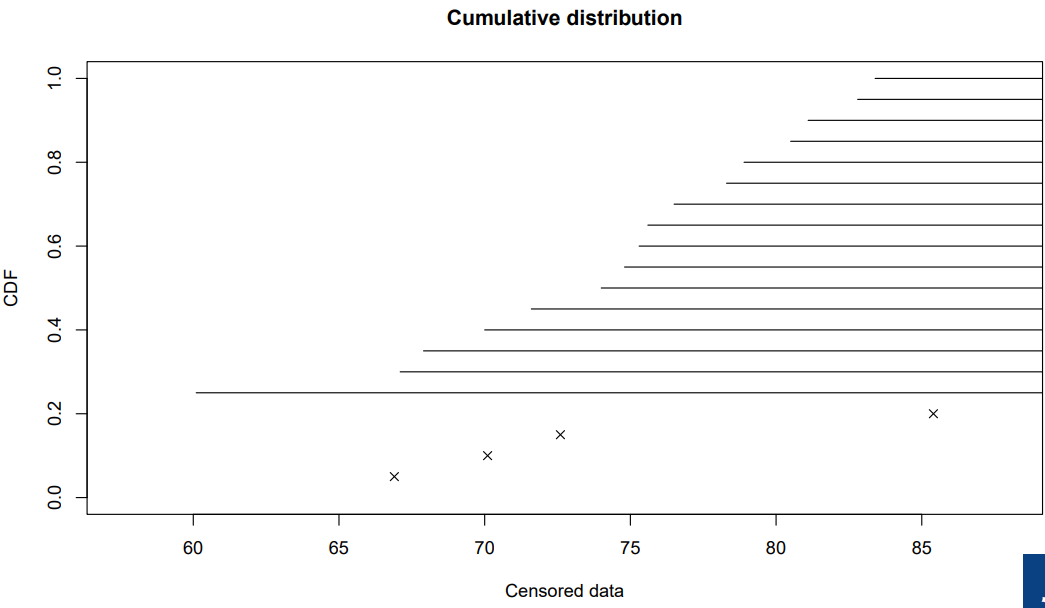
\includegraphics[width=0.7\linewidth]{right censor - raw cdf plot.png}
\end{figure}

\noi or as an empirical distribution
\begin{lstlisting}
fitdistrplus::plotdistcens(casdata)
\end{lstlisting}
\begin{figure}[H]
    \centering
    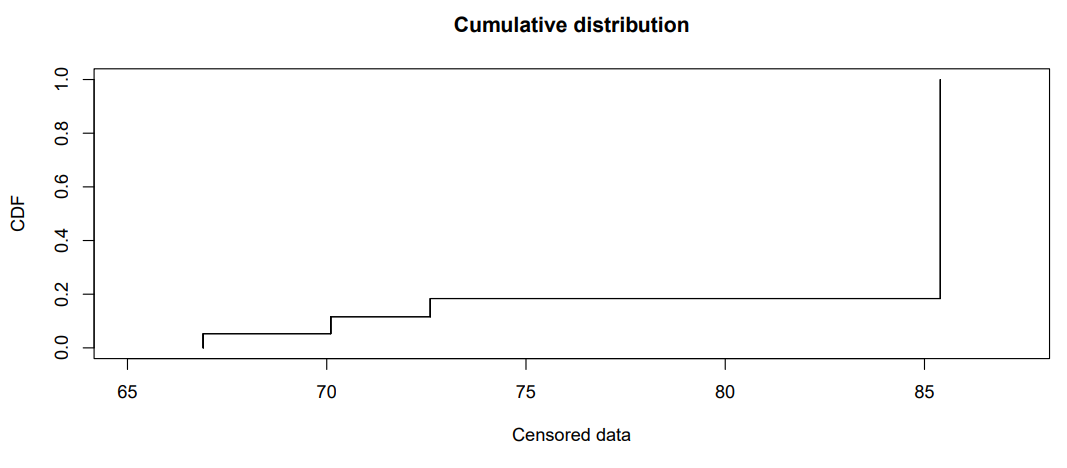
\includegraphics[width=0.7\linewidth]{right censor - raw data empirical plot.png}
\end{figure}

\subsubsection{Fitting censored data (in R)}
\begin{lstlisting}
cas.gamma.fit <- fitdistrplus::fitdistcens(casdata, "gamma")
summary(cas.gamma.fit)

## Fitting of the distribution ' gamma ' By maximum likelihood on censored## Parameters
##         estimate Std. Error
## shape 57.7678254 41.0552026
## rate   0.6629993  0.5059993
## Loglikelihood: -20.0179 AIC: 44.0358 BIC: 46.02727
## Correlation matrix:
## shape rate
## shape 1.0000000 0.9983085
## rate  0.9983085 1.0000000

plot(cas.gamma.fit)
\end{lstlisting}
\begin{figure}[H]
    \centering
    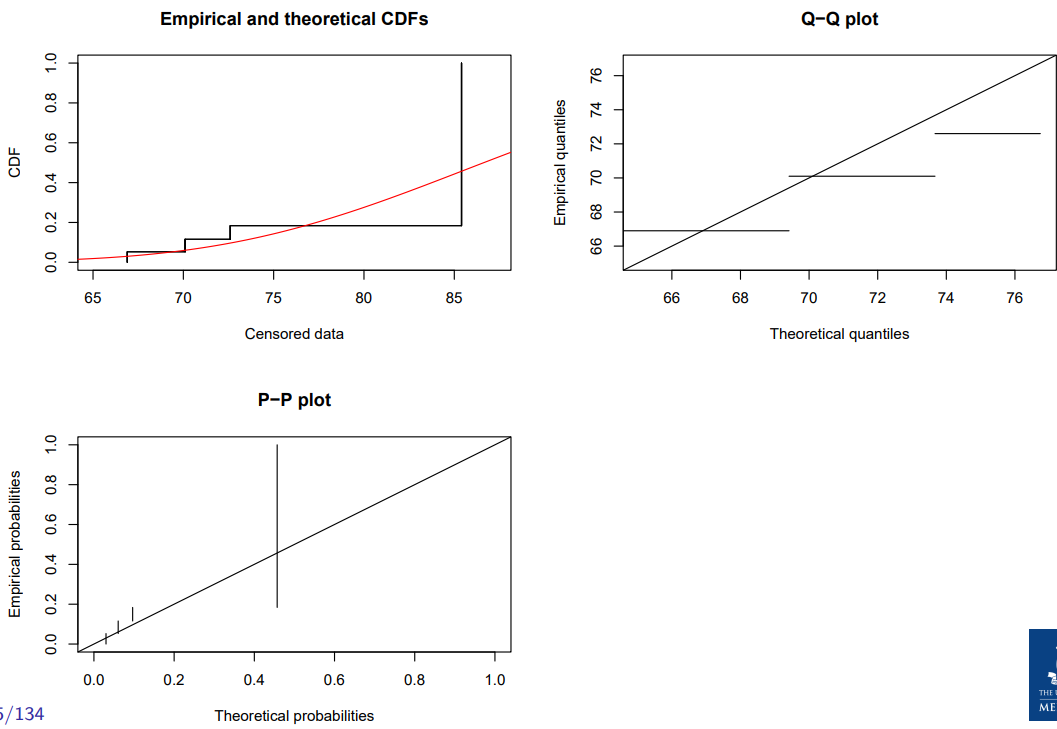
\includegraphics[width=0.7\linewidth]{right censor - fit data gamma.png}
\end{figure}

\subsubsection{Fitting left truncated data (in R)}
\noindent In actuarial work we often need to handle data that are recorded only if they lie in a window \((\,\ell,u]\).  If \(X\) has pdf \(f_X(x)\) and cdf \(F_X(x)\), then the \(\ell\)\!--left–truncated, \(u\)\!--right–truncated variable 
\[
Y \;=\; X \;\bigmid\; \{\ell<X\le u\}
\]
has density
\[
f_Y(y)
=\begin{cases}
\displaystyle
\frac{f_X(y)}{F_X(u)-F_X(\ell)}, 
&\ell<y\le u,\\[1em]
0,&\text{otherwise.}
\end{cases}
\]
Equivalently, its cdf is
\[
F_Y(y)=
\frac{F_X(y)-F_X(\ell)}{F_X(u)-F_X(\ell)},
\quad \ell<y\le u.
\]
\noindent\textbf{Comments:}
\begin{itemize}
  \item There is no built‐in R function for left‐truncation; one must adjust the likelihood manually by conditioning on \(X>\ell\).
  \item In the special cases \(\ell=-\infty\) or \(u=+\infty\) this reduces to simple one‐sided truncation.
  \item For interval‐censoring one uses the two‐column \texttt{(left,right)} coding shown earlier.
\end{itemize} \phantom{i}

\noi As an example in R, the \texttt{d} and \texttt{p} functions of a truncated exponential can
be coded as:
\begin{lstlisting}
dtexp <- function(x, rate, low, upp) {
    PU <- pexp(upp, rate = rate)
    PL <- pexp(low, rate = rate)
    dexp(x, rate)/(PU - PL) * (x >= low) * (x <= upp)
}

ptexp <- function(q, rate, low, upp) {
    PU <- pexp(upp, rate = rate)
    PL <- pexp(low, rate = rate)
    (pexp(q, rate) - PL)/(PU - PL) * (q >= low) * (q <= upp) + 1 * (q >
upp)
}
\end{lstlisting}

\noi If we generate 200 such truncated variables:
\begin{lstlisting}
set.seed(17032025)
n <- 200 # number of observations
x <- rexp(n) # simulating sample of x's
y <- x[x > 0.5 & x < 3] # truncating to get sample of y's
\end{lstlisting}

\noi and then fit them with either left- and right- truncation estimated from the data:
\begin{lstlisting}
fit.texp.emp <- fitdist(y, "texp", method = "mle", start = list(rate = 3),
    fix.arg = list(low = min(y), upp = max(y)))

# OR if you know the lower and upper bounds you can just manually replace it with 
# min(y) and max(y).
\end{lstlisting}

\subsubsection{When truncation and censoring levels are the same everywhere}
\begin{itemize}
    \item in R, the approach will be to code a left-truncated function, and then use the \texttt{foocens} functions.
    \item Let us do this on a gamma distribution:
\end{itemize}
\begin{lstlisting}
dtgamma <- function(x, rate, shape, low) {
        PL <- pgamma(low, rate = rate, shape = shape)
        dgamma(x, rate = rate, shape = shape)/(1 - PL) * (x >= low)
}

ptgamma <- function(q, rate, shape, low) {
        PL <- pgamma(low, rate = rate, shape = shape)
        (pgamma(q, rate = rate, shape = shape) - PL)/(1 - PL) * (q >= low)
}
\end{lstlisting}

\noi For instance, assume that truncated at $2$ and censored at $20$ for all data points.

\begin{lstlisting}
set.seed(22042021)
n <- 2000 # number of observations
x <- rgamma(n, shape = 2, rate = 0.2) # simulating sample of x's
x <- x[x > 2] # left-truncation at 2
n - length(x) # number of observations that were truncated
## [1] 123

censoring <- x > 20 # we will censor at 20
x[x > 20] <- 20 # censoring at 20

# Transform into right format
censoring[censoring == FALSE] <- x[censoring == FALSE]
censoring[censoring == TRUE] <- NA
xcens <- cbind.data.frame(left = x, right = censoring)

# And fitting (NOT alloowing for truncation):
fit.gamma.xcens <- fitdistcens(xcens, "gamma", start = list(shape =                                 mean(xcens$left)^2/var(xcens$left), rate = mean(xcens$left)/var(xcens$left)))
summary(fit.gamma.xcens)
## Fitting of the distribution ' gamma ' By maximum likelihood on censored## Parameters
##        estimate   Std. Error
## shape 2.7153083 0.089141066
## rate  0.2566683 0.009500217
## Loglikelihood: -5412.521 AIC: 10829.04 BIC: 10840.12

# And fitting (ALLOWING for truncation):
fit.tgamma.xcens <- fitdistcens(xcens, "tgamma", start = list(shape =                               mean(xcens$left)^2/var(xcens$left), rate = mean(xcens$left)/var(xcens$left)),
fix.arg = list(low = min(xcens$left)))
summary(fit.tgamma.xcens)
## Fitting of the distribution ' tgamma ' By maximum likelihood on censored## Parameters
##        estimate  Std. Error
## shape 2.0296237 0.10529978
## rate  0.2006534 0.01009728
## Fixed parameters:
##        value
## low 2.013575
## Loglikelihood: -5340.151 AIC: 10684.3 BIC: 10695.38

fitdistrplus::cdfcompcens(list(fit.gamma.xcens, fit.tgamma.xcens),
legendtext = c("Not allowing for truncation", "Allowing for truncation"))
\end{lstlisting}

\subsubsection{When truncation and censoring levels vary}
\noi In real life, an insurance product would have more than one level of
deductibles and limits to suit different policyholders. Simulating another
dataset:

\begin{lstlisting}
set.seed(2021)
n <- 3006 # number of observations 9 * 334
orig_x <- rgamma(n, shape = 2, rate = 0.2) # simulating sample of x's
deductibles = rep(c(rep(1, 3), rep(3, 3), rep(5, 3)), 334)
limits = rep(c(15, 20, 30), 3 * 334) + deductibles
# limit is on payment, not raw loss

# MANUALLY APPLYING THE DEDUCTIBLES AND LIMITS
x <- orig_x
censored <- x > limits # we will censor at the limits
x[censored] <- limits[censored] # censoring at the limits
# the above takes only elements of x which have TRUE in the vector
# censored
deducted <- x > deductibles
x <- x[deducted] # left-truncation at all points
# here the truncated observations disappear!
n - length(x) # observations that were truncated
## [1] 378
# that many were removed

claims <- data.frame(x = x, deduct = deductibles[deducted],
    limitI = censored[deducted])

# PRELIMINARY ANALYSIS
# randomising data, we pretend we do not know how the data was
# generated
claims <- claims[sample(1:nrow(claims), nrow(claims)), ]

hist(claims$x, breaks = 100)
# Note these includes right-censored observations but not the truncated
# values

# PREPARING OUR JOINT LOG LIKELIHOOD FUNCTION
# Here, we are minimising a negative log-likelihood instead of maximising a
# log-likelihood.

negloglik <- function(pdf, cdf, param, x, deduct, limitI) {
    # Function returns the negative log likelihood of the censored and
    # truncated dataset. Each data point's contribution to the log
    # likelihood depends on the theoretical distribution pdf and cdf
    # and also the deductible and limit values to adjust for truncation
    # and censoring
    
    PL <- do.call(cdf, c(list(q = deduct), param))
    PX <- do.call(cdf, c(list(q = x), param))
    fX <- do.call(pdf, c(list(x = x), param))
    
    lik.contr <- ifelse(limitI, log(1 - PX), log(fX)) - log(1 - PL)
    
    return(-sum(lik.contr))
}

# FITTING THE DISTRIBUTION
# Let’s try gamma. Note that our objective function needs starting values for
# the optimisation. What other starting values could we use?

pdf <- dgamma
cdf <- pgamma
x <- claims$x
deduct <- claims$deduct
limitI <- claims$limitI
# MME for starting values
start <- list(shape = mean(x)^2/var(x), rate = mean(x)/var(x))
obj.fun <- function(shape, rate) {
    param <- list(shape = shape, rate = rate)
    return(negloglik(pdf, cdf, param, x, deduct, limitI))
} # we now have a function to minimise wrt shape and rate

gamma.ll.fit <- stats4::mle(obj.fun, start = start, lower = c(0, 0))
summary(gamma.ll.fit)
## Maximum likelihood estimation
##
## Call:
## stats4::mle(minuslogl = obj.fun, start = start, lower = c(0,0))
##
## Coefficients:
##        Estimate   Std. Error
## shape 1.9867904 0.084680435
## rate  0.1963044 0.007726585
##
## -2 log L: 15140.45

param.g.ll <- stats4::coef(gamma.ll.fit)
param.g.ll
##     shape      rate
## 1.9867904 0.1963044

# TESTING HOW WELL WE WENT
fit.tcens.param <- param.g.ll # from the proper fit
fit.param <- coef(fitdist(claims$x, "gamma", method = "mle"))
# this is a naive fit

sim.tcens.gamma <- rgamma(10000, shape = fit.tcens.param[1],
rate = fit.tcens.param[2]) # sample from proper fit
sim.gamma <- rgamma(10000, shape = fit.param[1], rate = fit.param[2])
# sample from naive fit

# Comparing the proper fit (that accounts for l-trunc and r-cens) with
# a 'naive' fit (that does not account for those)
plot(ecdf(orig_x), main = "Empirical CDF plots", col = "black")
lines(ecdf(sim.tcens.gamma), col = "blue", type = "s")
lines(ecdf(sim.gamma), col = "red", type = "s")
legend("bottomright", legend = c("Original distribution",
    "Multilevel fit", "Naive fit"), lty = 1, col = c("black",
    "blue", "red"))
\end{lstlisting}
\begin{figure}[H]
    \centering
    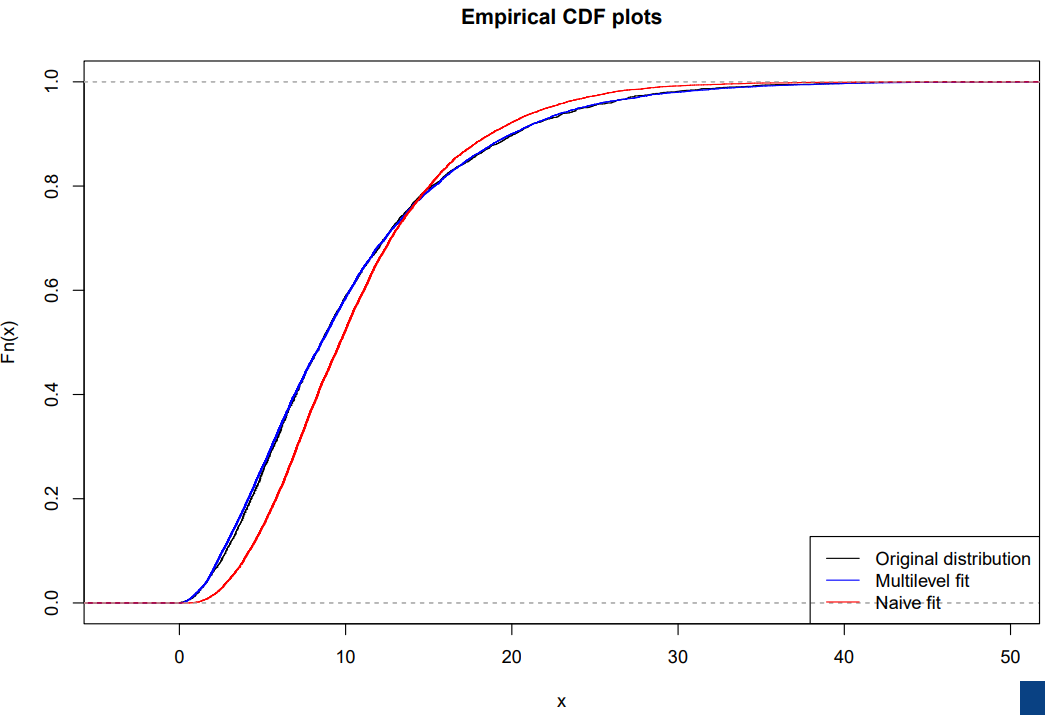
\includegraphics[width=0.7\linewidth]{l-trunc and r-cens final results plot.png}
\end{figure}

\subsection{Model Selection}
\subsubsection{Graphical Tool Diagnostics}

To assess the adequacy of a fitted parametric loss‐size model \(G(x;\widehat\theta)\), it is standard to use a suite of graphical checks:

\begin{enumerate}
  \item \textbf{Histogram \emph{vs.} fitted density.}  
    Overlay the histogram of the raw data \(\{y_i\}\) with the curve of the fitted density
    \[
      \widehat g(x) \;=\;\frac{\partial}{\partial x}G(x;\widehat\theta)\,.
    \]
    Look for major shape discrepancies (e.g.\ peak locations, tail thickness).

  \item \textbf{Empirical CDF \emph{vs.} fitted CDF.}  
    Plot the empirical CDF
    \[
      \widehat F_n(x)\;=\;\frac1n\sum_{i=1}^n\mathbf{1}\{y_i\le x\}
    \]
    against the theoretical CDF \(G(x;\widehat\theta)\).  Deviations from the \(45^\circ\) line indicate regions of poor fit.

  \item \textbf{P–P plot.}  
    For each ordered data point \(y_{(i)}\), plot
    \[
      \bigl(\,\widehat F_n(y_{(i)}),\;G(y_{(i)};\widehat\theta)\bigr).
    \]
    Points should lie close to the diagonal if the model is correct.

  \item \textbf{Q–Q plot.}  
    Let \(u_i = (i-0.5)/n\).  Plot the sample quantiles \(y_{(i)}\) against the theoretical quantiles
    \[
      G^{-1}(u_i;\widehat\theta)\,.
    \]
    A straight line indicates good agreement; curvature reveals systematic lack of fit in the center or tails.
\end{enumerate}

\noindent Together these plots provide a quick visual check for features such as skewness, tail weight, and multimodality that the model \(G(x;\widehat\theta)\) may fail to capture.  


\subsubsection{SUVA data Goodness of Fit Plots}
\begin{lstlisting}
plot.legend <- c("Weibull", "lognormal", "gamma")
fitdistrplus::denscomp(list(fit.weibull.mle, fit.lnorm.mle, fit.gamma.mle),
    legendtext = plot.legend, fitlwd = 3)
\end{lstlisting}
\begin{figure}[H]
    \centering
    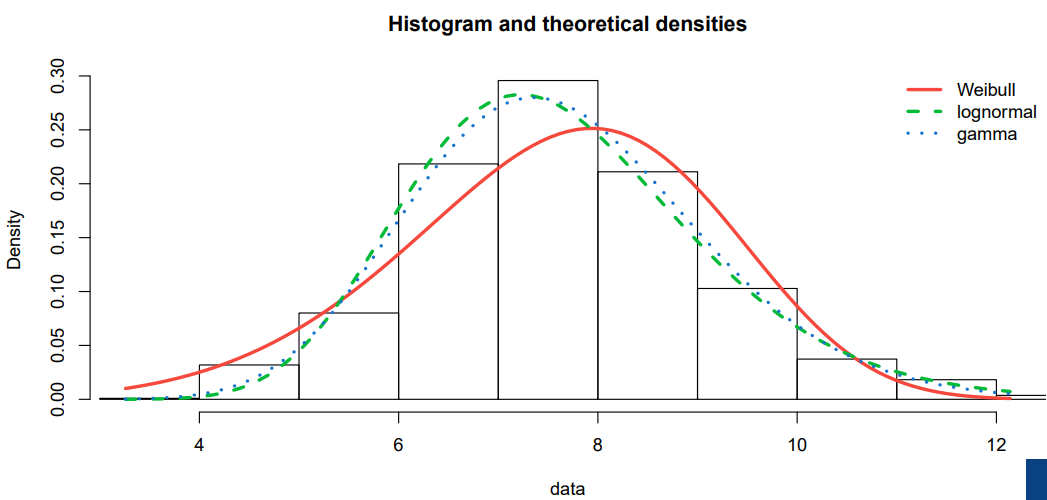
\includegraphics[width=0.7\linewidth]{SUVA - GOF - denscomp.png}
\end{figure}

\begin{lstlisting}
fitdistrplus::cdfcomp(list(fit.weibull.mle, fit.lnorm.mle,
    fit.gamma.mle), legendtext = plot.legend, fitlwd = 4, datapch = 20)
\end{lstlisting}
\begin{figure}[H]
    \centering
    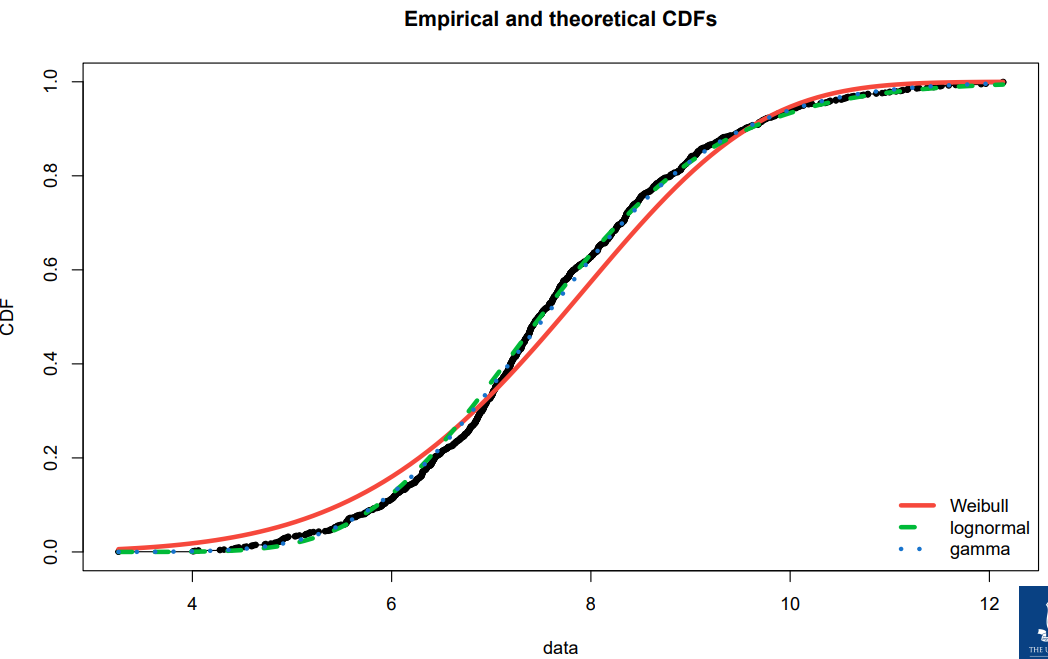
\includegraphics[width=0.7\linewidth]{SUVA - GOF - Emp and Theo CDF's.png}
\end{figure}

\begin{lstlisting}
fitdistrplus::ppcomp(list(fit.weibull.mle, fit.lnorm.mle,
    fit.gamma.mle), legendtext = plot.legend, fitpch = 20)
\end{lstlisting}
\begin{figure}[H]
    \centering
    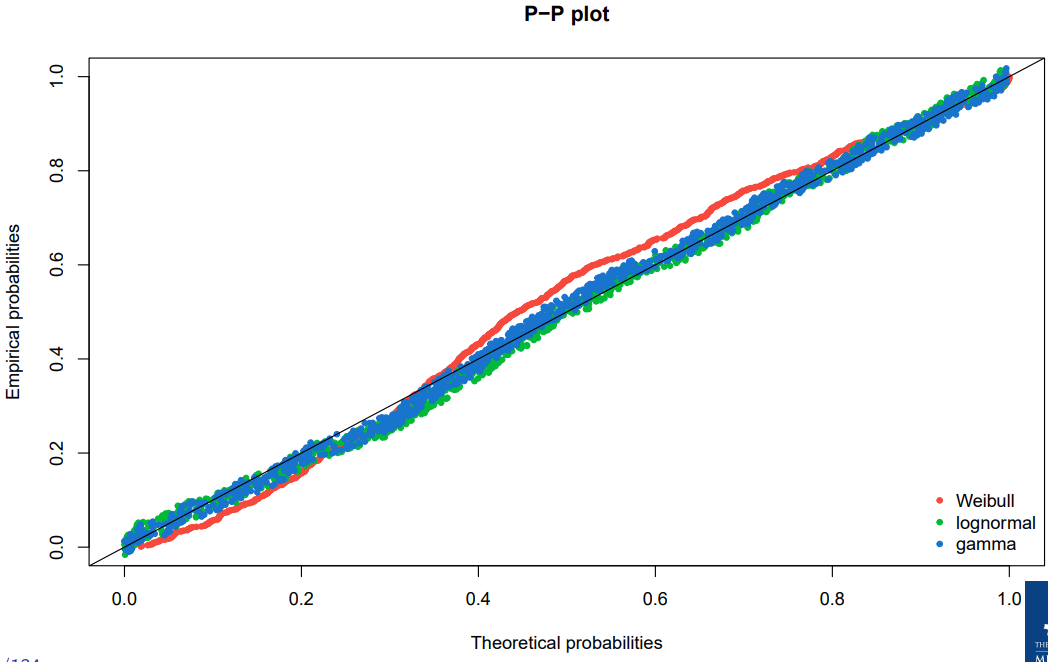
\includegraphics[width=0.7\linewidth]{SUVA - GOF - pp plot.png}
\end{figure}

\begin{lstlisting}
fitdistrplus::qqcomp(list(fit.weibull.mle, fit.lnorm.mle,
    fit.gamma.mle), legendtext = plot.legend, fitpch = 20)
\end{lstlisting}
\begin{figure}[H]
    \centering
    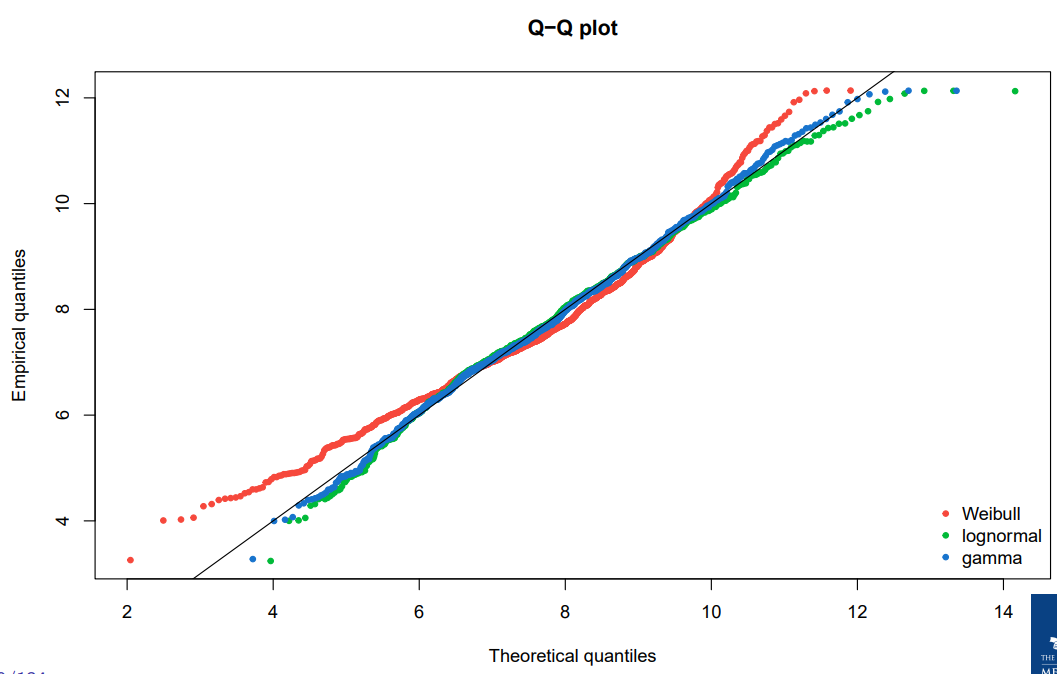
\includegraphics[width=0.7\linewidth]{SUVA - GOF - qq plot.png}
\end{figure}

\subsubsection{Hypothesis Tests}
\subsubsection{Hypothesis Tests for Goodness‐of‐Fit}

We test
\[
  H_0: \text{the data come from the fitted model }G(x;\widehat\theta),
  \quad
  H_a: \text{they do not}.
\]
Common test statistics are:
\begin{itemize}
  \item \textbf{Kolmogorov–Smirnov (K–S):}
    \[
      D = \sup_x\bigl|\widehat G_n(x) - G(x;\widehat\theta)\bigr|.
    \]
  \item \textbf{Anderson–Darling (A–D):}
    \[
      A^2
      = n \int_{-\infty}^{\infty}
        \frac{\bigl[\widehat G_n(x) - G(x;\widehat\theta)\bigr]^2}
             {G(x;\widehat\theta)\bigl[1 - G(x;\widehat\theta)\bigr]}\,
        dG(x;\widehat\theta).
    \]
  \item \(\boldsymbol{\chi^2}\) \textbf{goodness‐of‐fit:}
    \[
      \chi^2
      = \sum_{j}
        \frac{(\text{observed}_j - \text{expected}_j)^2}
             {\text{expected}_j},
    \]
    where the data are grouped into bins.
\end{itemize}

\subsubsection{Using the Test Statistics}

\begin{itemize}
  \item Among candidate models, prefer the one with
    \begin{itemize}
      \item smallest K–S statistic,
      \item smallest A–D statistic,
      \item smallest \(\chi^2\) (or equivalently largest \(p\)‐value),
      \item largest maximized log–likelihood \(\ell(\widehat\theta)\).
    \end{itemize}
  \item Note: K–S and A–D do \emph{not} adjust for the number of parameters; more complex models tend to fit better by these measures alone.
  \item The \(\chi^2\) test does adjust its degrees of freedom for the number of estimated parameters, but its results can be sensitive to the choice of binning.
\end{itemize}

\subsubsection{Model Selection via Information Criteria}

Information criteria penalize model complexity by adding a penalty to the (negative) log–likelihood.

\begin{itemize}
  \item \textbf{Akaike Information Criterion (AIC):}
    \[
      \mathrm{AIC} = -2\,\ell(\widehat\theta) + 2\,d,
    \]
    where \(d\) is the number of fitted parameters.
  \item \textbf{Bayesian Information Criterion (BIC):}
    \[
      \mathrm{BIC} = -2\,\ell(\widehat\theta) + \log(n)\,d,
    \]
    where \(n\) is the sample size.
\end{itemize} \phantom{i}

\noi Smaller AIC or BIC values indicate a preferred model.  As \(n\to\infty\), BIC tends to favor simpler models than AIC.  

\subsubsection{SUVA data Hypothesis Test Statistics}
\noi For MLE:
\begin{lstlisting}
gofstat(list(fit.weibull.mle, fit.lnorm.mle, fit.gamma.mle),
    fitnames = plot.legend)
## Goodness-of-fit statistics
##                                 Weibull   lognormal      gamma
## Kolmogorov-Smirnov statistic 0.07105097  0.04276791 0.03385082
## Cramer-von Mises statistic   1.74049707  0.26568341 0.19472283
## Anderson-Darling statistic   10.69572021 1.70209314 1.10574683
##
## Goodness-of-fit criteria
##                                   Weibull lognormal gamma
## Akaike's Information Criterion 4010.519 3920.717 3907.637
## Bayesian Information Criterion 4020.524 3930.722 3917.641
\end{lstlisting}

\noi For MME:
\begin{lstlisting}
## Goodness-of-fit statistics
##                                 Weibull  lognormal     gamma
## Kolmogorov-Smirnov statistic 0.08023228  0.0374087 0.0327241
## Cramer-von Mises statistic   1.66608962  0.1869752 0.1823197
## Anderson-Darling statistic   10.53097690 1.4369047 1.0539353
##
## Goodness-of-fit criteria
##                                 Weibull lognormal   gamma
## Akaike's Information Criterion 4044.239 3922.121 3907.677
## Bayesian Information Criterion 4054.243 3932.125 3917.681
\end{lstlisting}

\noi R can also provide the results from the GOF hypothesis tests. For example:
\begin{lstlisting}
gammagof <- gofstat(list(fit.gamma.mle, fit.lnorm.mle),
    fitnames = c("gamma MLE", "lognormal MLE"),
    chisqbreaks = c(10:20/2))
gammagof$chisqpvalue
##    gamma MLE lognormal MLE
## 1.378914e-03 1.690633e-05

gammagof$adtest
## gamma MLE lognormal MLE
## "rejected" "not computed"

gammagof$kstest
## gamma MLE lognormal MLE
## "not rejected" "rejected"

gammagof$chisqtable
## obscounts theo gamma MLE theo lognormal MLE
## <= 5 36 23.98533 19.19169
## <= 5.5 28 39.67114 39.53512
## <= 6 60 72.80478 76.73318
## <= 6.5 110 109.49748 116.38286
## <= 7 130 139.03929 145.08202
## <= 7.5 191 152.62215 154.45787
## <= 8 134 147.60896 144.65495
## <= 8.5 141 127.75620 121.96771
## <= 9 91 100.23486 94.30131
## <= 9.5 62 72.06145 67.84850
## <= 10 51 47.90581 45.97086
## > 10 65 65.81255 72.87394
\end{lstlisting}

\subsection{Calculating Within Layers of Claim Size}
\subsubsection{Deductibles and Policy Limits}

Let \(X\) be the \emph{ground‐up} loss.  We introduce two main features:

\begin{itemize}
  \item \textbf{Deductible} \(d\): the insurer only pays the excess above \(d\).  Define
  \[
    Y = 
    \begin{cases}
      0,             & X \le d,\\
      X - d,         & X > d,
    \end{cases}
    \quad\Longrightarrow\quad
    Y = (X - d)_{+} \;=\;\max(X - d,0).
  \]
  \item \textbf{Policy limit} \(M\): the insurer pays up to \(M\).  Define
  \[
    Y =
    \begin{cases}
      X,             & X \le M,\\
      M,             & X > M,
    \end{cases}
    \quad\Longrightarrow\quad
    Y = X \wedge M \;=\;\min(X,M).
  \]
\end{itemize}

Combining both a deductible \(d\) and a limit \(M\), the insurer’s payment is
\[
  Y = \min\bigl\{\,(X-d)_{+},\,M\bigr\}
  = \min\bigl\{\,X \wedge (d+M)\bigr\} - \bigl(X \wedge d\bigr).
\]

\subsubsection{Useful Formulas for Truncated Moments}

\paragraph{First moment of the capped loss.}
\[
  \mathbb{E}[\,X \wedge M\,]
    = \int_{0}^{M} x\,f_X(x)\,dx \;+\; M\bigl[1 - F_X(M)\bigr]
    \quad\text{(continuous \(X\))},
\]
\[
  \mathbb{E}[\,X \wedge M\,]
    = \sum_{i: x_i\le M} x_i\,P(X=x_i)\;+\;M\bigl[1 - F_X(M)\bigr]
    \quad\text{(discrete \(X\))}.
\]

Equivalently, using the survival function \(S_X(x)=1 - F_X(x)\):
\[
  \mathbb{E}[\,X \wedge M\,]
    = \int_{0}^{M} S_X(x)\,dx,
    \quad
  \mathbb{E}[\,X \wedge M\,]
    = \sum_{i:0\le x_i < M} S_X(x_i)\,\bigl(x_{i+1}-x_i\bigr).
\]

\paragraph{\(k\)th moment of the capped loss.}
\[
  \mathbb{E}\bigl[\,(X \wedge M)^k\bigr]
    = \int_{0}^{M} x^k\,f_X(x)\,dx \;+\; M^k\bigl[1 - F_X(M)\bigr]
    \quad\text{(continuous)},
\]
\[
  \mathbb{E}\bigl[\,(X \wedge M)^k\bigr]
    = \sum_{i: x_i\le M} x_i^k\,P(X=x_i)\;+\;M^k\bigl[1 - F_X(M)\bigr]
    \quad\text{(discrete)}.
\]

\subsubsection{Reinsurance}
Reinsurance is a \emph{risk transfer} from an insurer to a reinsurer: the insurer ced es some of its random risk in exchange for a (deterministic) premium.  The part the insurer keeps is called the \emph{retention}.

\subsubsection{Types of Reinsurance}

\begin{itemize}
  \item \textbf{Proportional}
    \begin{itemize}
      \item \emph{Quota share}: same fixed proportion for every risk.
      \item \emph{Surplus}: insurer retains up to a fixed line per risk; excess is ceded.
    \end{itemize}
  \item \textbf{Non–proportional}
    \begin{itemize}
      \item \emph{Excess–of–loss}: on each individual loss \(X_i\), reinsurer covers \((X_i - d)_{+}\).
      \item \emph{Stop–loss}: on aggregate loss \(S = \sum_{i=1}^N X_i\), reinsurer covers \((S - d)_{+}\).
    \end{itemize}
  \item \textbf{Alternative Risk Transfers (ART)}: e.g.\ CAT‐bonds, longevity bonds, pandemic bonds.
\end{itemize}

\subsubsection{Proportional Reinsurance}

If the retained fraction is \(\alpha\in[0,1]\), then for ground‐up loss \(X\):
\[
  Y \;=\;\alpha\,X,
  \qquad
  Z \;=\;(1-\alpha)\,X.
\]
Hence
\[
  \mathbb{E}[Y] \;=\;\alpha\,\mathbb{E}[X],
  \quad
  \text{Var}(Y) \;=\;\alpha^2\,\text{Var}(X),
  \quad
  \gamma_Y = \gamma_X.
\]
\paragraph{Example.} If \(X\sim\mathrm{Exp}(\beta)\), then
\[
  \Pr[Y \le y]
  = \Pr[\alpha X \le y]
  = \Pr\bigl[X \le y/\alpha\bigr]
  = 1 - e^{-\beta\,y/\alpha},
\]
so \(Y\sim\mathrm{Exp}(\beta/\alpha)\).

\subsubsection{Non–Proportional Reinsurance}

\paragraph{Individual Loss Cover}  
For each loss \(X_i\):
\[
  Y_i = \min(X_i,\,d),
  \quad
  Z_i = (X_i - d)_{+}.
\]
With an upper limit \(M\), one may write
\[
  Y_i = \min(X_i,d) + (X_i - d - M)_{+},
  \quad
  Z_i = \min\bigl((X_i - d)_{+},\,M\bigr).
\]
The insurer retains \(\sum_i Y_i\), the reinsurer pays \(\sum_i Z_i\).

\paragraph{Aggregate (Stop–Loss) Cover}  
On total loss \(S=\sum_{i=1}^N X_i\):
\[
  Y = \min(S,\,d),
  \quad
  Z = (S - d)_{+},
  \quad
  P_d \;=\;\mathbb{E}[(S-d)_{+}],
\]
where \(P_d\) is known as the \emph{stop–loss premium}.  With an aggregate limit \(M\):
\[
  Y = \min(S,d) + (S - d - M)_{+},
  \quad
  Z = \min\bigl((S - d)_{+},\,M\bigr).
\]

\subsubsection{Mixed Truncation/Censoring on Retention}

Suppose the underlying ground‐up loss \(D\) is left‐truncated at \(d\) and right‐censored at \(u\).  Then the insurer’s payment
\[
  X = 
  \begin{cases}
    D - d, & d \le D < u,\\
    u - d, & D \ge u,
  \end{cases}
\]
has mixed density
\[
  f_X(x)
   =
  \begin{cases}
    \displaystyle
    \frac{f_D(x+d)}{1 - F_D(d)}, 
    & 0 < x < u - d,\\[6pt]
    \displaystyle
    \frac{1 - F_D(u)}{1 - F_D(d)},
    & x = u - d,\\
    0,&\text{otherwise.}
  \end{cases}
\]
In \textsf{R} you can then call  
\verb|coverage(pdf=dgamma,cdf=pgamma,deductible=2,limit=20)|  
 ($d=2, \ u=20$) to get the corresponding density ($f_{X}(x)$) for fitting.

\begin{lstlisting}
fit.gamma.xcens2 <- MASS::fitdistr(xcens$left - 2, f,
    start = list(shape = mean(xcens$left)^2/var(xcens$left),
        rate = mean(xcens$left)/var(xcens$left)))
fit.gamma.xcens2
##    shape         rate
## 2.03990496    0.20142871
## (0.10516140) (0.01009694)

fit.tgamma.xcens # our previous fit with fitdist
## Fitting of the distribution ' tgamma ' on censored data by maximum likelihood
## Parameters:
##        estimate
## shape 2.0296237
## rate  0.2006534
## Fixed parameters:
##        value
## low 2.013575

c(fit.gamma.xcens2$loglik, fit.tgamma.xcens$loglik)
## [1] -5341.551 -5340.151
\end{lstlisting}












\newpage
%%%%%%%%%%%%%%%%%%%%%%%%%%%%%%%%%%%%%%%%%%%%%%%%%%%%%%%%%%%%%%%%%%%%%%%%%%%%%%
\section{Module 4 – Approximations for Compound Distributions}

\subsection{The \((a,b,0)\) class of distributions}
\noi The \((a,b)\) class of Panjer distributions has the following recursion property:
\[
p_k \;=\;\Pr[N=k]
\;=\;\Bigl(a+\frac{b}{k}\Bigr)\Pr[N=k-1]
\;=\;\Bigl(a+\frac{b}{k}\Bigr)p_{k-1},
\quad k=1,2,\dots
\]
or equivalently,
\[
\frac{p_k}{p_{k-1}}
= a+\frac{b}{k},
\quad k=1,2,\dots
\]
\noi Hence \(\Pr[N=k]\) can be computed recursively from the initial value \(p_0=\Pr[N=0]\).

\begin{table}[ht]
\centering
\caption{Members of the \((a,b,0)\) class}
\vspace{0.5em}
\begin{tabular}{|c|c|c|c|}
\hline
\thead{Distribution} & \thead{$a$} & \thead{$b$} & \thead{$\Pr[N=0]$} \\
\hline
Poisson\;($\lambda$)          & $0$                   & $\lambda$               & $e^{-\lambda}$           \\
NegBin\;($\gamma,p$)          & $p$                   & $(\gamma-1)\,p$         & $(1-p)^{\gamma}$         \\
Binomial\;($\nu,p$)           & $-\dfrac{p}{1-p}$     & $(\nu+1)\,\dfrac{p}{1-p}$ & $(1-p)^{\nu}$           \\
\hline
\end{tabular}
\end{table}

\subsubsection*{Example: Poisson and Binomial}
\noi For the Poisson pmf,
\[
\frac{\Pr[N=n]}{\Pr[N=n-1]}
=\frac{e^{-\lambda}\,\lambda^n/n!}{e^{-\lambda}\,\lambda^{n-1}/(n-1)!}
=\frac{\lambda}{n}
=0+\frac{\lambda}{n},
\]
\noi so 
\[
a=0,\qquad b=\lambda.
\]

\noi For the Binomial pmf,
\[
\frac{\Pr[N=n]}{\Pr[N=n-1]}
=\frac{\binom{\nu}{n}p^n(1-p)^{\nu-n}}
      {\binom{\nu}{n-1}p^{n-1}(1-p)^{\nu-n+1}}
=\frac{\nu-n+1}{n}\,\frac{p}{1-p}
=\frac{p}{1-p}\Bigl(-1+\frac{\nu+1}{n}\Bigr)
=-\frac{p}{1-p}+\frac{(\nu+1)p}{1-p}\,\frac{1}{n},
\]
\noi so
\[
a=-\frac{p}{1-p},\qquad b=\frac{(\nu+1)p}{1-p}.
\]

\subsection{The \((a,b,1)\) class of distributions}
\noi A discrete random variable is a member of the \((a,b,1)\) class of distributions if there exist constants \(a\) and \(b\) such that
\[
\frac{p_k}{p_{k-1}}
= a + \frac{b}{k},
\quad k = 2,3,\dots.
\]
\noi Note:
\begin{itemize}
  \item The recursion starts at \(k=2\) for the \((a,b,1)\) class.
  \item The extra freedom allows the probability at zero to be set to any value \(0 \le p_0 \le 1\).
\end{itemize}

\subsubsection{Zero‐truncated distributions}
\noi Setting $p_0=0$ in the \((a,b,1)\) class defines the subclass of \textbf{zero‐truncated distributions}.  Let $p_k^T$ denote the probability mass at $k$ for a zero‐truncated distribution.  Then
\[
p_k^T
=\begin{cases}
0\,,&k=0,\\[0.3em]
\dfrac{p_k}{1-p_0}\,,&k=1,2,\dots,
\end{cases}
\]
where $p_k$ is the pmf of the corresponding member of the \((a,b,0)\) class.  

\noi Members include:
\begin{itemize}
  \item zero‐truncated Poisson (\texttt{actuar::ztpois}),
  \item zero‐truncated binomial (\texttt{actuar::ztbinom}),
  \item zero‐truncated negative binomial (\texttt{actuar::ztnbinom}),
  \item zero‐truncated geometric (\texttt{actuar::ztgeom}).
\end{itemize}

\subsubsection{Zero‐modified distributions}
\noi Setting \(p_0\equiv p_0^M\) \(\bigl(0<p_0^M<1\bigr)\) in the \((a,b,1)\) class defines the subclass of \textbf{zero‐modified distributions}.  These distributions are discrete mixtures between a degenerate mass at zero and the corresponding \((a,b,0)\) member.  Let \(p_k^M\) denote the probability mass at \(k\) for a zero‐modified distribution.  Then
\[
p_k^M
=\begin{cases}
p_0^M, & k = 0,\\[0.3em]
\dfrac{1 - p_0^M}{\,1 - p_0\,}\;p_k, & k = 1,2,\dots,
\end{cases}
\]
where \(p_k\) is the pmf of the corresponding member of the \((a,b,0)\) class.  

\noi Members include the zero‐modified
\begin{itemize}
  \item Poisson (\texttt{actuar::zmpois}),
  \item Binomial (\texttt{actuar::zmbinom}),
  \item Negative binomial (\texttt{actuar::zmnbinom}),
  \item Geometric (\texttt{actuar::zmgeom}).
\end{itemize} \phantom{i}

\begin{lstlisting}
plot(dpois(0:7, 2.5), pch = 20, col = "red", ylim = c(0, 0.3),
cex = 1.5, type = "b")
points(dztpois(0:7, 2.5), pch = 20, col = "blue", type = "b")
points(dzmpois(0:7, 2.5, 2 * dpois(0, 2.5)), pch = 20, col = "green",
type = "b")
\end{lstlisting}

\begin{figure}[H]
    \centering
    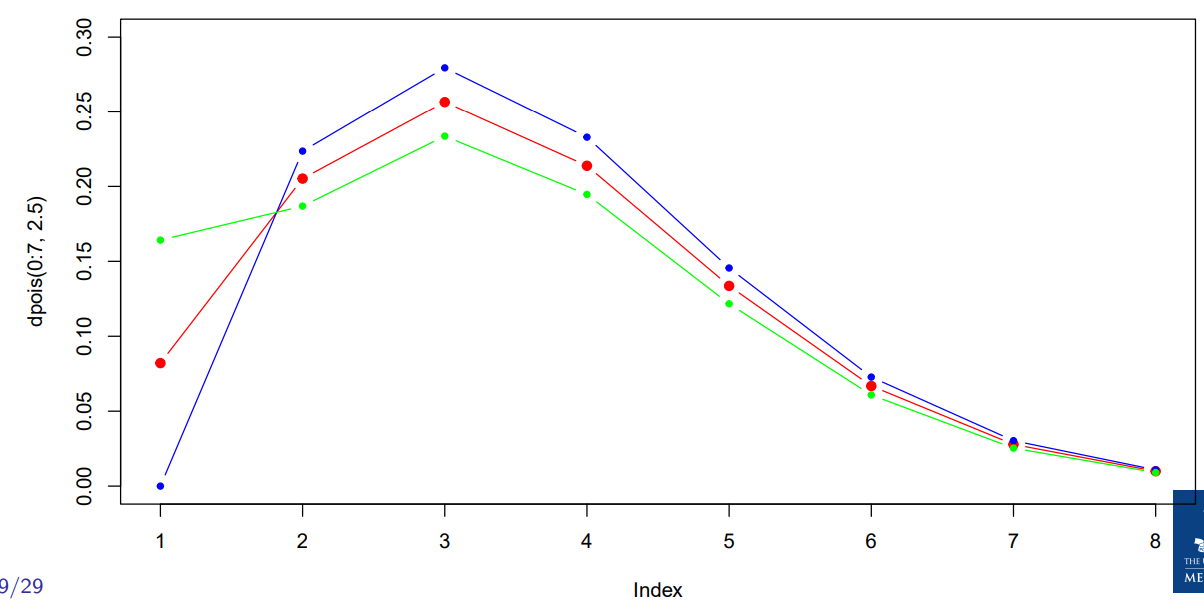
\includegraphics[width=0.7\linewidth]{zero-modified dist R example.png}
\end{figure}

\subsection{Panjer’s recursion algorithm}
\noi
\begin{itemize}
  \item The remarkable property of the \((a,b)\) class of frequency distributions allows us to develop a \emph{recursive} method to get the distribution of \(S\) for discrete \(Y\)'s.
  \item When \(Y\) is continuous, simply discretise its cdf first.
\end{itemize} \phantom{i}

\noi Let \(S\) have a compound distribution on \(Y\), i.e.\ \(S=\sum_{i=1}^N Y_i\), where the following are mutually independent:
\begin{itemize}
  \item \(N\) belongs to the \((a,b)\) class of distributions;
  \item the \(Y_i\) are i.i.d., non‐negative and discrete with pmf \(g_j=\Pr(Y=j)\).
\end{itemize}
\noi Then for \(s=1,2,\dots\),
\[
f_S(s)
=\frac{1}{1 - a\,g_0}
\sum_{j=1}^{s}
\Bigl(a + \frac{b\,j}{s}\Bigr)\,g_j\,f_S(s-j),
\]
with starting value
\[
f_S(0)
=\begin{cases}
\Pr(N=0), & g_0=0,\\[0.3em]
M_N\bigl(\ln g_0\bigr), & g_0>0,
\end{cases}
\]
\noi where \(M_N(t)=E[e^{tN}]\) is the mgf of \(N\).  Note that if \(g_y=0\) for \(y>y_{\max}\), the upper limit of the sum may be replaced by \(\min(s,y_{\max})\).

\subsubsection*{Example: Panjer’s recursion for compound Poisson}
\noi If \(S\sim\) compound Poisson\((\lambda,\{g_j\})\), then \(N\) is Poisson with parameters \(a=0,b=\lambda\) so Panjer’s formula gives for \(s=1,2,\dots\)
\[
f_S(s)
=\frac{\lambda}{s}
\sum_{j=1}^{s}j\,g_j\,f_S(s-j),
\]
with starting value (whether \(g_0\) is zero or not)
\[
f_S(0)
=\exp\!\bigl[\lambda\,(g_0-1)\bigr].
\]

\subsubsection*{Example 12.4.2 (Bowers et al., 1997)}
\noi Let \(N\sim\Poisson(\lambda=0.8)\), and let claim sizes \(Y_i\) be i.i.d.\ with
\[
\Pr(Y=1)=0.25,\quad
\Pr(Y=2)=0.375,\quad
\Pr(Y=3)=0.375.
\]
Define the aggregate loss
\[
S=\sum_{i=1}^N Y_i.
\]
Use Panjer’s recursion to compute \(f_S(s)=\Pr(S=s)\) for \(s=0,1,2,3,\dots\). \\

\noi\textbf{Solution.}  Here \(a=0\), \(b=\lambda=0.8\), and \(g_j=\Pr(Y=j)\).  Panjer’s recursion gives
\[
f_S(s)
=\frac{\lambda}{s}\sum_{j=1}^{s}j\,g_j\,f_S(s-j),
\quad s=1,2,\dots,
\]
with starting value
\[
f_S(0)=\Pr(N=0)=e^{-0.8}=0.44933.
\]
Hence
\[
f_S(1)
=\frac{0.8}{1}\bigl(1\cdot0.25\,f_S(0)\bigr)
=0.2\,e^{-0.8}
=0.089866,
\]
\[
f_S(2)
=\frac{0.8}{2}\bigl(1\cdot0.25\,f_S(1)+2\cdot0.375\,f_S(0)\bigr)
=0.32\,e^{-0.8}
=0.14379,
\]
\[
f_S(3)
=\frac{0.8}{3}\bigl(1\cdot0.25\,f_S(2)+2\cdot0.375\,f_S(1)+3\cdot0.375\,f_S(0)\bigr)
=0.3613\,e^{-0.8}
=0.16236,
\]
etc. \\

\noi In R:
\begin{lstlisting}
fs <- actuar::aggregateDist(method = "recursive", model.freq = "poisson",
lambda = 0.8, model.sev = c(0, 0.25, 0.375, 0.375), x.scale = 1)
diff(fs)[1:4]
fs(knots(fs)) # supposed to return cdf, haven't tested but is in documentation

## [1] 0.44932896 0.08986579 0.14378527 0.16235753

plot(fs)
\end{lstlisting}

\begin{figure}[H]
    \centering
    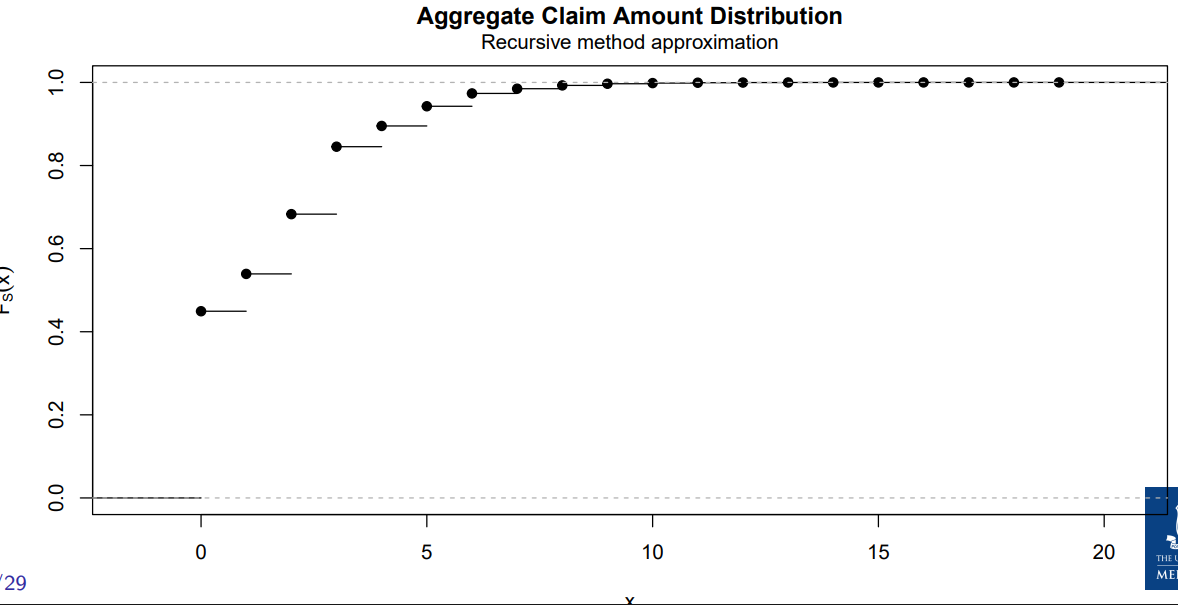
\includegraphics[width=0.75\linewidth]{Panjer Recursion Aggregate Claim Example.png}
\end{figure}

\subsubsection{Panjer’s recursion in R}
\noi Panjer’s recursion can be performed using the \texttt{aggregateDist} function with \texttt{method="recursive"}.
\begin{itemize}
  \item The frequency distribution can be any member of the \((a,b,0)\) or \((a,b,1)\) class (i.e.\ with arbitrary mass at zero).
  \item The severity distribution must be discrete on \(\{0,1,\dots,m\}\) for some monetary unit.
\end{itemize}
\noi Important parameters include:
\begin{itemize}
  \item \texttt{model.freq}: name of the frequency distribution (e.g.\ \texttt{"poisson"}, \texttt{"nbinom"}, etc.).
  \item \texttt{model.sev}: data frame or named vector giving the pmf of the discretized severity distribution \(Y\).
  \item \texttt{x.scale}: the value of one monetary unit in the severity model (i.e.\ the increment size of the support).
  \item \texttt{diff(model)}: returns a vector of the pmf values.
  \item \texttt{model(knots(model))}: returns a vector of cdf evaluated at knots.
\end{itemize}

\subsection{Approximations}

Possible motivations for using approximations to the compound distribution \(S\):
\begin{itemize}
  \item Exact computation of the distribution of \(S\) may be infeasible:
    \begin{itemize}
      \item no detailed data beyond the moments of \(S\),
      \item technical difficulties in fitting a tractable model.
    \end{itemize}
  \item A sophisticated model may be wrong (limited data, etc.) and an approximation can be sufficiently accurate.
  \item Quick results are needed, or high precision is not justified by available resources.
\end{itemize}

\noindent\textbf{Notation:} In this section we write
\[
s_S \equiv \gamma_1(S), 
\qquad
\gamma_2(S)\equiv\gamma_2.
\]

\subsubsection{Normal approximation}

By the Central Limit Theorem,
\[
\Pr[S\le s]
=\Pr\Bigl[\frac{s - \mathbb{E}[S]}{\sqrt{\Var(S)}} \le Z\Bigr]
\approx \Phi\!\Bigl(\frac{s - \mathbb{E}[S]}{\sqrt{\Var(S)}}\Bigr),
\]
where \(Z\sim N(0,1)\) and \(\Phi\) is its cdf.

\begin{itemize}
  \item The classical CLT holds for a fixed number of summands, whereas here \(N\) is random.
  \item In the special case \(S\sim\mathrm{CompPoi}(\lambda\nu,G)\), Theorem 4.1 of Wüthrich (2024) shows
  \[
    \frac{S - \lambda\nu\,\mathbb{E}[Y]}{\sqrt{\lambda\nu\,\mathbb{E}[Y^2]}}
    \;\Longrightarrow\;N(0,1)
    \quad(\nu\to\infty),
  \]
  leading to
  \[
    \Pr[S\le s]\approx
    \Phi\!\Bigl(\frac{s - \lambda\nu\,\mathbb{E}[Y]}{\sqrt{\lambda\nu\,\mathbb{E}[Y^2]}}\Bigr).
  \]
  This requires \(\mathbb{E}[Y^2]<\infty\), so is best used for \(S_{sc}\).
\end{itemize}

\subsubsection{Translated Gamma and Log‐Normal approximations}

\textbf{Idea:}  Instead of correcting the CLT, choose a positively skewed distribution and match its first three moments via a location parameter \(k\).  Let
\[
X = k + Z,
\quad
Z\sim
\begin{cases}
\Gamma(\gamma,c),\\
\mathrm{Lognormal}(\mu,\sigma^2).
\end{cases}
\]
Match \(\mathbb{E}[X]=\mathbb{E}[S]\), \(\Var(X)=\Var(S)\), and skewness \(\gamma_1(X)=s_S\).  Here \(k\) only enters the mean.

\paragraph{Fitting a translated gamma to \(S\sim\mathrm{CompPoi}(\lambda\nu,G)\):}  
We solve
\[
\begin{cases}
\mathbb{E}[S]=\lambda\nu\,\mathbb{E}[Y] = k + \gamma/c,\\[0.3em]
\Var(S)=\lambda\nu\,\mathbb{E}[Y^2] = \gamma/c^2,\\[0.3em]
s_S
=\displaystyle\frac{\mathbb{E}[Y^3]}{(\lambda\nu)^{1/2}\,\mathbb{E}[Y^2]^{3/2}}
=2\,\gamma^{-1/2}.
\end{cases}
\]
Hence
\[
\gamma
=\Bigl(\frac{2(\lambda\nu)^{1/2}\,\mathbb{E}[Y^2]^{3/2}}{\mathbb{E}[Y^3]}\Bigr)^2,
\quad
c=\Bigl(\frac{\gamma}{\lambda\nu\,\mathbb{E}[Y^2]}\Bigr)^{1/2},
\quad
k=\lambda\nu\,\mathbb{E}[Y]-\frac{\gamma}{c}.
\]

\subsubsection*{Example: Normal and translated Gamma approximation}

Suppose \(S\sim\mathrm{CompPoi}(\lambda=16,\,Y\equiv1)\).  Find \(\Pr(S\le25)\) by both methods.

\paragraph{Normal approximation}
\[
\Pr(S\le25)
\approx \Phi\!\Bigl(\frac{25-16}{\sqrt{16}}\Bigr)
=\Phi(2.25)
=0.98776.
\]

\paragraph{Translated Gamma approximation}
Here \(\nu=1\) and \(Y\equiv1\implies\mathbb{E}[Y]=1\), \(\mathbb{E}[Y^2]=1\), \(\mathbb{E}[Y^3]=1\).  The moment‐matching equations become
\[
\frac{\gamma}{c}+k=16,
\quad
\frac{\gamma}{c^2}=16,
\quad
2/\sqrt{\gamma}=1/4,
\]
whence
\(\gamma=64\), \(c=2\), \(k=-16\).  Thus
\[
\Pr(S\le25)
\approx \Pr(X<25)=\Pr(Z<25-k)=\Pr(Z<41),
\quad Z\sim\Gamma(64,2),
\]
\[
\Pr(Z<41)
=\frac{2^{64}}{\Gamma(64)}\int_{0}^{41}x^{63}e^{-2x}\,dx
=\mathrm{pgamma}(41,64,2)
=0.98252.
\]


\newpage
%%%%%%%%%%%%%%%%%%%%%%%%%%%%%%%%%%%%%%%%%%%%%%%%%%%%%%%%%%%%%%%%%%%%%%%%%%%%%%
\section{Module 5 - Copulas}
\subsection{Measures of dependence}
Independence $\implies$ zero correlation BUT zero correlation $\nRightarrow$ independence.

\subsubsection{Pearson's correlation measure}
\noi Pearson's correlation coefficient is defined by
$$\rho(Z_i, Z_j) = \rho_{ij} = \frac{\text{Cov}(Z_i, Z_j)}{\sqrt{\text{Var}(Z_i)\text{Var}(Z_j)}}$$
\noi Note:
\begin{itemize}
    \item this measures the degree of \textbf{linear relationship} between $Z_i$ and $Z)j$.
    \item its value is between $-1$ and $1$.
    \item in general, it does not reveal all the information of the dependence structure of random couples.
\end{itemize}
\begin{lstlisting}
cor(data, method = "pearson") # default, data needs to have more than 1 column
\end{lstlisting}

\subsubsection{Kendall's tau}
\noi Kendall's tau rank correlation coefficient is defined by
$$\tau(Z_i, Z_j) = \tau_{ij} = \Pr[(Z_i-Z_i')(Z_j-Z_j')>0] - \Pr[(Z_i - Z_i')(Z_j-Z_j') < 0]$$
\noi where ($Z_i, Z_j$) and ($Z_j, Z_j'$) are two independent realisations.

\noi Note:
\begin{itemize}
    \item the first term is called the probability of concordance, the latter, probability of disconcordance.
    \item its value is also between $-1$ and $1$.
    \item it can be shown to equal: $\tau(Z_i, Z_j) = 4\mathbb{E}[F(Z_i, Z_j)] - 1$.
    \item concordance and disconcordance only depends on \textbf{ranks}.
\end{itemize}
\begin{lstlisting}
cor(data, method = "kendall") # data needs to have more than 1 column
# Kendall's tau is unchanged under transformations that do not affect rank (eg. log)
\end{lstlisting}

\subsubsection{Spearman's rho}
\noi Spearman's rho rank correlation coefficient is defined by
$$r(Z_i, Z_j) = r_{ij} = \rho(F_i(Z_i), F_j(Z_j))$$
\noi where $F_i$ and $F_j$ are the respective marginal distributions. Note:
\begin{itemize}
    \item it is a measure of Pearson's correlatoin but applied to the transformed variables.
    \item its value is also between $-1$ and $1$.
    \item it is directly formulated on ranks.
\end{itemize}
\begin{lstlisting}
cor(data, method = "spearman") # data needs to have more than 1 column
# Kendall's tau is unchanged under transformations that do not affect rank (eg. log)
\end{lstlisting}

\subsection{Copula Theory}
\subsubsection{Sklar's representation theorem}
\noi Copula links the joint distribution function to its marginals. Skalr's theorem says there exists a copula function C such that:
$$F(x_1,x_2,...,x_n) = C(F_1(x_1),F_2(x_2),...,F_n(x_n))$$
\noi where $F_k$ is the marginal df of $X_k$, $k=1,2,...,n$. Equivalently,
$$\Pr(X_1\leq x_1, ..., X_n \leq x_n) = C(\Pr[X_1 \leq x_1],...,\Pr[X_n \leq n_n]$$

\noi An $n$-dimensional copula is a df on $[0,1]^n$ with standard uniform marginal distributions.\\
 
\noi Under certain conditions, the copula:
$$C(u_1,...,u_n) = \Pr[U_1 \leq F_1(X_1),..., U_n \leq F_n(X_n)] = F(F_1^{-1}(u_1),...,F_n^{-1}(u_n))$$
\noi is unique, where $F_k^{-1}$ denote the quantile functions.

\subsubsection{When is a Copula valid}
\noi For $n = 2$, $C$ is a function mapping $[0,1]^2$ to $[0,1]$ that is non-decreasing and right continuous, and:
\begin{enumerate}
    \item $\displaystyle \lim_{u_k\to 0}C(u_1,u_2)=0$ for $k=1,2$;
    \item $\displaystyle \lim_{u_1\to 1}C(u_1,u_2)=u_2$ and $\displaystyle \lim_{u_2\to 1}C(u_1,u_2)=u_1$;
    \item $C$ satisfies the inequality
    $$
        C(v_1,v_2)-C(u_1,v_2)-C(v_1,u_2)+C(u_1,u_2)\ge 0
        \quad\text{for any }u_1\le v_1,\ u_2\le v_2.
    $$
\end{enumerate}

\noi Corresponding heuristics are:
\begin{enumerate}
    \item If the event on one variable is impossible, then the joint probability is impossible.
    \item If the event on one variable is certain, then the joint probability boils down to the marginal of the other one.
    \item There cannot be negative probabilities.
\end{enumerate}

\subsubsection{Constructing Copulas from df's examples}
\noi \textbf{Example 1}:
\noi Let
\[
F(x,y)=
\begin{cases}
\displaystyle \frac{(x+1)(e^y-1)}{x+2e^y-1}, & (x,y)\in[-1,1]\times[0,\infty),\\[0.5em]
1-e^{-y}, & (x,y)\in(1,\infty)\times[0,\infty),\\[0.5em]
0, & \text{elsewhere}.
\end{cases}
\]
\noi Hence
\[
F(x,\infty)=F(x)=\frac{x+1}{2}\equiv u,\quad x\in[-1,1],
\qquad
F^{-1}(u)=2u-1=x,
\]
\[
F(1,y)=G(y)=1-e^{-y}\equiv v,\quad y\ge0,
\qquad
G^{-1}(v)=-\ln(1-v)=y.
\]
\noi Finally,
\begin{align*}
C(u,v)
&=\frac{(2u-1+1)\bigl[(1-v)^{-1}-1\bigr]}{2u-1+2\bigl((1-v)^{-1}-1\bigr)}
=\frac{2u(1-1+v)}{(2u-2)(1-v)+2}\\
&=\frac{2uv}{2u-2uv-2+2v+2}
=\frac{uv}{u+v-uv}
=uv\times\frac{1}{u+v-uv}.
\end{align*}
\noi Note:
\begin{itemize}
    \item Independence copula is $C(u,v)=uv$, here “tweaked” by a function of $u$ and $v$.
    \item The copula captures the dependence structure, while separating the effects of the marginals (which are behind probabilities $u$ and $v$).
    \item Other copulas generally contain parameter(s) to fine-tune the strength of dependence.
\end{itemize} \phantom{i}

\noi \textbf{Example 2}:
\noi Suppose $(X_1,X_2)$ has a bivariate distribution function described by
\[
F(X_1\le x_1,\;X_2\le x_2)
=\exp\!\Bigl\{-\bigl[\bigl(\log\tfrac{1}{1-e^{-x_1}}\bigr)^\alpha
+\bigl(\log\tfrac{1}{1-e^{-x_2}}\bigr)^\alpha\bigr]^{1/\alpha}\Bigr\},
\quad \alpha\ge1.
\]
Derive the marginal distributions of $X_1$ and $X_2$ and express the copula function $C$ such that
\[
F(X_1\le x_1,X_2\le x_2)
=C\bigl(F_{X_1}(x_1),F_{X_2}(x_2)\bigr)
=C(u,v).
\]

\noi By letting $x_2\to\infty$, we find the marginal of $X_1$:
\[
F_{X_1}(x_1)=F(x_1,\infty)=1-e^{-x_1}=u.
\]
Similarly, by letting $x_1\to\infty$, we find the marginal of $X_2$:
\[
F_{X_2}(x_2)=F(\infty,x_2)=1-e^{-x_2}=v.
\]
Both have Exp(1) distribution. We then have
\[
C(u,v)
=F(X_1\le x_1,X_2\le x_2)
=\exp\!\bigl\{-\bigl[(-\log u)^\alpha+(-\log v)^\alpha\bigr]^{1/\alpha}\bigr\}.
\]

\subsubsection{Invariance property of Copulas}
\noi
\begin{itemize}
    \item Suppose random vector $\mathbf{X}$ has copula $C$ and suppose $T_1,\dots,T_n$ are strictly increasing functions of $X_1,\dots,X_n$, respectively.
    \item The random vector defined by $(T_1(X_1),\dots,T_n(X_n))$ has the same copula $C$—this is referred to as the \textbf{invariance property}.
    \item The usefulness of this property can be illustrated in many ways. If you have a copula describing joint distribution of insurance losses of various types, and you decide the quantity of interest is a transformation (e.g.\ logarithm) of these losses, then the multivariate distribution structure does not change.
    \item The copula is then also invariant to inflation.
    \item Only the marginal distributions change.
\end{itemize}

\subsubsection{The Fr\'echet Bounds}
\noi Define the Fréchet bounds as:
\begin{itemize}
    \item \textbf{Fréchet lower bound:} 
    \[
        L_F(u_1,\dots,u_n)
        =\max\Bigl(\sum_{k=1}^n u_k - (n-1),\,0\Bigr)
    \]
    \item \textbf{Fréchet upper bound:} 
    \[
        U_F(u_1,\dots,u_n)
        =\min(u_1,\dots,u_n)
    \]
\end{itemize}
\noi All copula satisfy the following bounds:
\[
    L_F(u_1,\dots,u_n)\;\le\;C(u_1,\dots,u_n)\;\le\;U_F(u_1,\dots,u_n).
\]

\subsubsection{Fundamental copulas}
\noi Fundamental copulas contain special dependence structures.
\begin{itemize}
    \item The independence copula introduced earlier $\Pi(u,v)=uv$ reflects the independence (i.e., lack of dependence) of the rvs.
    \item The \textbf{comonotonicity} copula is the Fréchet upper bound copula with
    \[
        M(u,v)=\min(u,v).
    \]
    \begin{itemize}
        \item This special copula is the joint df of random vector $(V,V)$ where $V\sim\mathrm{Uniform}(0,1)$, reflecting the \textbf{perfectly positive dependence} structure of the rvs.
        \item In other words, there is a single source of risk and the comonotonic variables are some increasing transformations of that risk.
    \end{itemize}
    \item The \textbf{countermonotonicity} copula is the Fréchet lower bound copula with
    \[
        W(u,v)=\max(u+v-1,0).
    \]
    \begin{itemize}
        \item This special copula is the joint df of random vector $(V,1-V)$ where $V\sim\mathrm{Uniform}(0,1)$, reflecting the \textbf{perfectly negative dependence} structure of the rvs.
    \end{itemize}
    \item The Fréchet upper bound satisfies the definition of a copula, but the Fréchet lower bound does not for dimensions $n\ge3$. In other words, the countermonotonicity copula only exists for dimension $n=2$, whereas the comonotonicity copula can be obtained for dimensions $n\ge2$.
\end{itemize}

\subsubsection{Survival copulas}
\noi What if we want to work with survival functions
\[
\overline{F}_i(x_i)=1 - F_i(x_i)=S_i(x_i)
\]
rather than distribution functions?\\
$\to$ We can couple the $\overline{F}_i$’s with the \textbf{survival copula} $\overline{C}$.\\

\noi In the bivariate case, this yields
\[
\overline{F}(x_1,x_2)
=\Pr[X_1>x_1,\;X_2>x_2]
=\overline{C}\bigl(\overline{F}_1(x_1),\;\overline{F}_2(x_2)\bigr),
\]
where
\[
\overline{C}(1-u,1-v)=1-u-v+C(u,v).
\]
This is because
\[
\Pr[X_1>x_1,X_2>x_2]
=1-\Pr[X_1\le x_1]-\Pr[X_2\le x_2]
+\Pr[X_1\le x_1,X_2\le x_2].
\]

\subsection{Tail Dependence}
\subsubsection{Coefficient of Lower Tail Dependence}
\noi The coefficient of \textbf{lower tail dependence} is defined as
\[
\lambda_L
=\lim_{u\to0^+}
\Pr\bigl[X_1 \le F_{X_1}^{-1}(u)\,\big|\,X_2 \le F_{X_2}^{-1}(u)\bigr]
=\lim_{u\to0^+}\frac{C(u,u)}{u},
\]
\noi where $\lambda_L\in[0,1]$.\\

\noi Examples:
\[
\lambda_L^{\Pi}
=\lim_{u\to0^+}\frac{u\cdot u}{u}
=\lim_{u\to0^+}u=0,
\qquad
\lambda_L^{M}
=\lim_{u\to0^+}\frac{\min(u,u)}{u}
=\lim_{u\to0^+}1=1.
\]

\subsubsection{Coefficient of Upper Tail Dependence}
\noi The coefficient of \textbf{upper tail dependence} is defined similarly but using the survival copula, which yields
\[
\lambda_U
=\lim_{u\to1^-}
\Pr\bigl[X_1\ge F_{X_1}^{-1}(u)\,\big|\,X_2\ge F_{X_2}^{-1}(u)\bigr]
=\lim_{u\to1^-}\frac{\overline{C}(1-u,1-u)}{1-u}
=\lim_{u\to0^+}\frac{\overline{C}(u,u)}{u}.
\]
\noi Note $\overline{C}(u,u)=2u-1+C(1-u,1-u)$ and $\lambda_U\in[0,1]$.\\
\noi Examples:
\[
\lambda_U^{\Pi}
=\lim_{u\to1^-}\frac{1-2u+u^2}{1-u}
=\lim_{u\to1^-}(1-u)=0,
\qquad
\lambda_U^{M}
=\lim_{u\to1^-}\frac{1-2u+\min(u,u)}{1-u}
=\lim_{u\to1^-}1=1.
\]

\subsection{Archimedean copulas}
\noi $C$ is \textbf{Archimedean} if it has an explicit closed‐form
\[
C(u_1,\dots,u_n)
=\psi^{-1}\bigl(\psi(u_1)+\cdots+\psi(u_n)\bigr),
\]
for all $0\le u_1,\dots,u_n\le1$ and for some continuous function $\psi$ (called the \emph{generator}) satisfying:
\begin{enumerate}
    \item $\psi(1)=0$;
    \item $\psi$ is strictly decreasing ($\psi'(t) < 0$); and
    \item $\psi$ is convex ($\psi''(t) \geq 0$).
\end{enumerate} \phantom{i}

\noi The Kendall’s $\tau$ and the generator function $\psi(t)$ are related via
\[
\tau \;=\;1+4\int_{0}^{1}\frac{\psi(t)}{\psi'(t)}\,dt \in [-1,1]
\]
\noi \texit{Note}: 
\begin{itemize}
    \item If $\tau = -1$ it is counter-monotonicity copula since it is perfectly dis-concordant (perfectly negatively correlated).
    \item If $\tau = 1$ it is co-monotonicity copula since it is perfectly concordant (perfectly positively correlated).
\end{itemize}

\subsubsection{Clayton Copula}
\noi The bivariate Clayton copula is defined by
\[
C(u_1,u_2)
=\bigl(u_1^{-\theta}+u_2^{-\theta}-1\bigr)^{-1/\theta},
\qquad \theta\in(0,\infty).
\]
\noi It is of Archimedean type with:
\begin{itemize}
    \item $\displaystyle \psi(t)=\frac{1}{\theta}\bigl(t^{-\theta}-1\bigr)$
    \item $\displaystyle \psi^{-1}(s)=\bigl(1+\theta\,s\bigr)^{-1/\theta}$
\end{itemize}
\noi The relationship between Kendall’s $\tau$ and $\theta$ is
\[
\tau=\frac{\theta}{2+\theta}
\quad\Longleftrightarrow\quad
\theta=\frac{2\tau}{1-\tau}.
\]
\noi The tail‐dependence coefficients are
\[
\lambda_L
=\lim_{u\to0^+}\frac{C(u,u)}{u}
=2^{-1/\theta},
\qquad
\lambda_U
=\lim_{u\to1^-}\frac{\overline{C}(1-u,1-u)}{1-u}
=0.
\]
\noi \textbf{Limiting cases:}
\begin{itemize}
    \item As $\theta\to0$, 
    \[
        C(u,v)\;\to\;uv,
    \]
    the independence copula.
    \item As $\theta\to\infty$, 
    \[
        C(u,v)\;\to\;\min(u,v),
    \]
    the comonotonicity copula.
    \item (Bivariate only) Extending to $\theta\to(-1)^+$ yields 
    \[
        C(u,v)\;\to\;\max(u+v-1,0),
    \]
    the countermonotonicity copula.
\end{itemize}


\subsubsection{Frank copula}
\noi The bivariate Frank copula is defined by
\[
C(u_1,u_2)
=-\frac{1}{\theta}\,
\ln\!\Biggl(
1+\frac{(e^{-\theta u_1}-1)\,(e^{-\theta u_2}-1)}{e^{-\theta}-1}
\Biggr),
\qquad \theta\in\mathbb{R}\setminus\{0\}.
\]
\noi It is of Archimedean type with:
\begin{itemize}
  \item $\displaystyle \psi(t)
    =-\ln\!\Bigl(\tfrac{e^{-\theta t}-1}{\,e^{-\theta}-1}\Bigr)$,
  \item $\displaystyle \psi^{-1}(s)
    =-\tfrac{1}{\theta}\ln\!\bigl(1+e^{-s}(e^{-\theta}-1)\bigr)$.
\end{itemize}
\noi The relationship between Kendall’s $\tau$ and $\theta$ is
\[
\tau
=1-\frac{4}{\theta}+\frac{4}{\theta^2}
\int_{0}^{\theta}\frac{t}{e^t-1}\,dt.
\]
\noi The tail‐dependence coefficients are
\[
\lambda_L
=\lim_{u\to0^+}\frac{C(u,u)}{u}
=0,
\qquad
\lambda_U
=\lim_{u\to1^-}\frac{\overline{C}(1-u,1-u)}{1-u}
=0.
\]
\noi \textbf{Limiting cases:}
\begin{itemize}
  \item As $\theta\to0$, 
    \[
      C(u,v)\;\to\;uv,
    \]
    the independence copula.
  \item As $\theta\to+\infty$, 
    \[
      C(u,v)\;\to\;\min(u,v),
    \]
    the comonotonicity copula.
  \item As $\theta\to-\infty$, 
    \[
      C(u,v)\;\to\;\max(u+v-1,0),
    \]
    the countermonotonicity copula (bivariate only).
\end{itemize}


\subsubsection{Gumbel Copula}
\noi The bivariate Gumbel–Hougaard copula is defined by
\[
C(u_1,u_2)
=\exp\!\Bigl(-\bigl[(-\ln u_1)^\theta+(-\ln u_2)^\theta\bigr]^{1/\theta}\Bigr),
\qquad \theta\in[1,\infty).
\]
\noi It is of Archimedean type with:
\begin{itemize}
  \item $\displaystyle \psi(t)=\bigl(-\ln t\bigr)^\theta$,
  \item $\displaystyle \psi^{-1}(s)=\exp\bigl(-s^{1/\theta}\bigr)$.
\end{itemize}
\noi The relationship between Kendall’s $\tau$ and $\theta$ is
\[
\tau=\frac{\theta-1}{\theta}
\quad\Longleftrightarrow\quad
\theta=\frac{1}{1-\tau}.
\]
\noi The tail‐dependence coefficients are
\[
\lambda_L
=\lim_{u\to0^+}\frac{C(u,u)}{u}
=0,
\qquad
\lambda_U
=\lim_{u\to1^-}\frac{\overline{C}(1-u,1-u)}{1-u}
=2-2^{1/\theta}.
\]
\noi \textbf{Limiting cases:}
\begin{itemize}
  \item $\theta=1\implies C(u,v)=uv$, the independence copula.
  \item $\theta\to\infty\implies C(u,v)\to\min(u,v)$, the comonotonicity copula.
\end{itemize}




\newpage
%%%%%%%%%%%%%%%%%%%%%%%%%%%%%%%%%%%%%%%%%%%%%%%%%%%%%%%%%%%%%%%%%%%%%%%%%%%%%%
\section{Module 6 – Extreme Value Theory (EVT)}
\subsection{Measures of tail weight}
\noi Models that assign higher probabilities to these large values are said to be heavier-tailed. Tail behaviour can be examined via
\begin{enumerate}
    \item \textbf{log-log plot}: linear decrease for heavy tails
    \item \textbf{Mean Excess function}: linear increase for heavy tails
    \item \textbf{Existence of Moments}: Less moments means more heavy tails (e.g. Pareto vs. gamma)
    \item \textbf{Limiting Density Ratio}: ratio of density function as the right tail of two distributions
        $$\lim_{x \rightarrow \infty}{\frac{S_A(x)}{S_B(x)}} = \lim_{x\rightarrow\infty}{\frac{f_A(x)}{f_B(x)}}$$
        \begin{itemize}
            \item If limit = $c$ (constant): The tails are comparable in size
            \item If limit = $\infty$: Distribution $A$ has a heavy tail than $B$
            \item If limit = $0$: Distribution $A$ has a thinner tail than $B$
        \end{itemize}
    \item \textbf{Hazard Rate function}: $h(x) = \frac{f(x)}{1-F(x)}$, constant for exponential and decreasing for heavy tails.
\end{enumerate}

\subsubsection*{Example: Exponential vs. Pareto (limit of survival functions)}
\begin{align*}
    \lim_{x \rightarrow \infty}{\frac{S_{\text{Pareto}}(x)}{S_{\text{Exponential}}(x)}} &= \lim_{x\rightarrow\infty}\frac{\frac{\theta^\alpha}{(x+\theta)^\alpha}}{e^{-\theta x}} \\
    &= \lim_{x\rightarrow\infty}\frac{\theta^\alpha e^{\theta x}}{(x+\theta)^\alpha} \rightarrow \infty \text{, so pareto has heavier tail}
\end{align*}

\subsubsection*{Example: Exponential vs. Pareto (hazard rate function)}
\begin{align*}
    h_{(\text{exp})}(x) &= \frac{\frac{1}{\theta}e^{-\frac{x}{\theta}}}{e^{-\frac{x}{\theta}}} \\
    &= \frac{1}{\theta} \text{, (constant)} \\
    &\quad \\
    h_{(\text{pareto})}(x) &= \frac{\alpha \frac{\theta^\alpha}{(x+\theta)^{\alpha+1}}}{\frac{\theta^\alpha}{(x+\theta)^\alpha}} \\
    &= \frac{\alpha}{x+\theta} \text{, (decreasing in $x$ so heavier tail)}
\end{align*}

\subsubsection*{Example: Limiting density ratio - Gamma}
\begin{figure}[H]
    \centering
    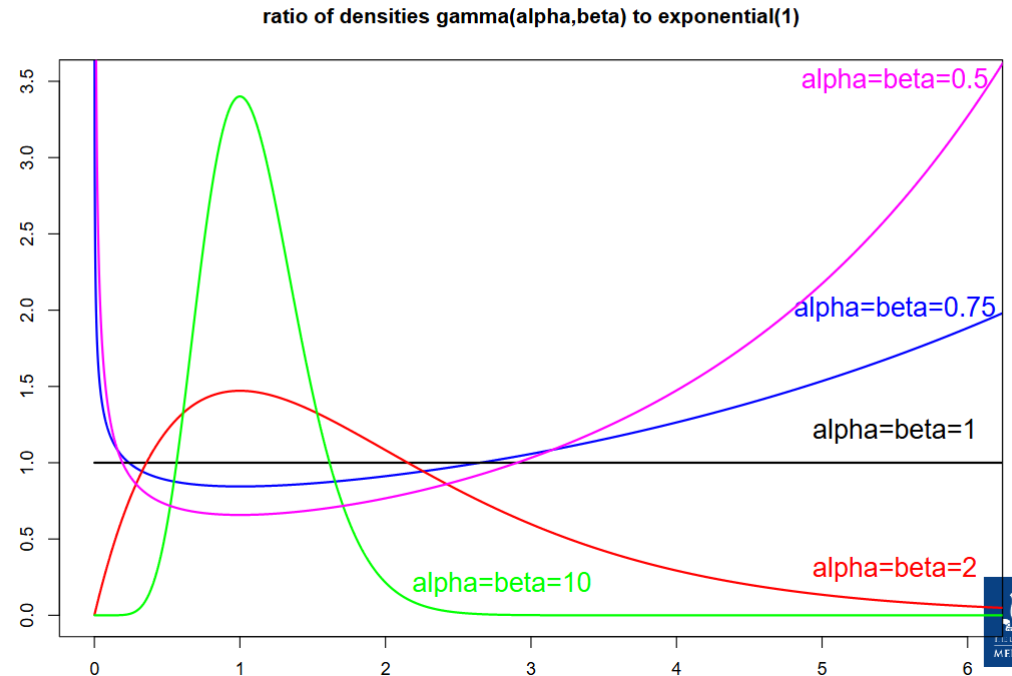
\includegraphics[width=0.7\linewidth]{Limiting density ratio - gamma example.png}
\end{figure}
\begin{itemize}
    \item $\alpha > 1 \implies$ thinner tail than exponential
    \item $\alpha < 1 \implies$ fatter tail than exponential
\end{itemize}

\subsubsection*{Example: Hazard rate function - Gamma with fixed mean}
\begin{figure}[H]
    \centering
    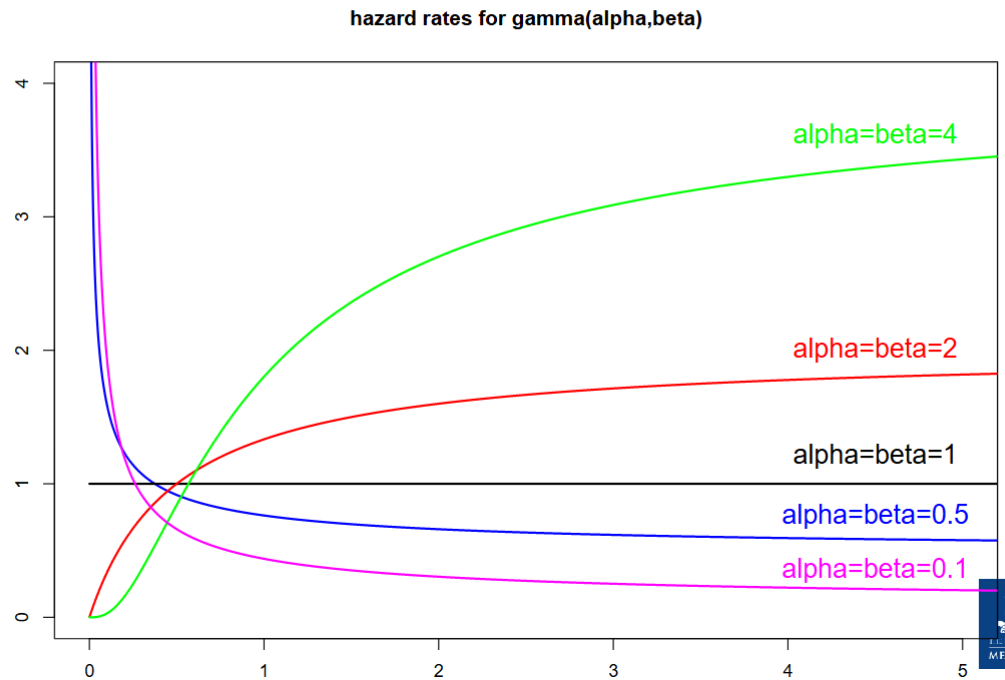
\includegraphics[width=0.7\linewidth]{Hazard rate function - gamma example.png}
\end{figure}

\subsection{Framework: n-block maximum}
\begin{itemize}
    \item Consider iid random variables $X_i$, $i=1,...,$, with df $F$
    \item Denote the order statistics
        $$X_{n,n} \leq X_{n-1,n} \leq ... \leq X_{1,n}$$
        such that 
        $$X_{n,n} = \min(X_1,...,X_n) \text{ and } X_{1,n} = \max(X_1,...,X_n)$$
\end{itemize}

\subsubsection{Parallel with CLT}
\begin{itemize}
    \item In the exponential example, the normalised maximum
        $$\frac{X_{1,n}}{\text{mean of } X} - \log n$$
        for infinite sample $n$ stabilised to a Gumbel distribution $\Lambda$.
    \item This generalises to any distribution $X$ -- the limiting distribution of the normalised maximum then becomes a Generalised Extreme Value (GEV) distribution.
\end{itemize}

\subsection{GEV Distribution}
$$H_{\gamma; \ \mu, \sigma}(x) = \begin{cases}
    e^{-(1 + \gamma \frac{x- \mu}{\sigma})^{-\frac{1}{\gamma}}} &, \gamma \neq 0 \\
    e^{-e^{-\frac{x-\mu}{\sigma}}} &, \gamma = 0
\end{cases}$$
\noi $\mu \in \mathbb{R}$ and $\sigma > 0$ \\

\noi There are three cases:
\begin{itemize}
    \item $\gamma < 0$: upper bounded Weibull with $x < \mu - \sigma/\gamma$
    \item $\gamma = 0$: Gumbel with $x \in \mathbb{R}$
    \item $\gamma > 0$: Fr\'echet with $x > \mu - \sigma/\gamma$ (heavy tailed distributions, right tail)
\end{itemize}

\begin{table}[ht]
\centering
\caption{GEV distributions (for the maximum value) corresponding to common loss distributions}
\vspace{0.5em}
\begin{tabular}{|c|>{\centering\arraybackslash}m{4cm}|>{\centering\arraybackslash}m{4.5cm}|>{\centering\arraybackslash}m{4cm}|}
\hline
\thead{Type} & \thead{WEIBULL \\ $\gamma < 0$} & \thead{GUMBEL \\ $\gamma = 0$} & \thead{FRÉCHET \\ $\gamma > 0$} \\
\hline
\makecell{\textbf{Underlying} \\ \textbf{Distribution}} & 
\makecell{Beta \\ Uniform \\ Triangular} & 
\makecell{Chi-square \\ Exponential \\ Gamma \\ Log-normal \\ Normal \\ Weibull} & 
\makecell{Burr \\ $F$ \\ Log-gamma \\ Pareto \\ $t$} \\
\hline
\makecell{\textbf{Range of values} \\ \textbf{permitted}} & 
$x < \mu - \dfrac{\sigma}{\gamma}$ & 
$-\infty < x < \infty$ & 
$x > \mu - \dfrac{\sigma}{\gamma}$ \\
\hline
\end{tabular}
\end{table}

\subsubsection{Example: Exponential}
\noi For underlying cdf $F(x) = 1 - e^{-\beta x}$, for $\beta>0$ and $x \geq 0$, the GEV form $H$ can be obtained by:

\begin{align*}
    \lim_{x\rightarrow\infty}{\Pr\Big[\frac{X_{1,n} - b_n}{a_n} \leq x\Big]} &= \lim_{x\rightarrow\infty}{\Pr[X_{1,n} \leq a_nx + b_n]} \\
    &= \lim_{x\rightarrow\infty}{F(a_n x + b_n)^n} \\
    &= \lim_{x\rightarrow\infty}{\Big( 1 - e^{-\beta(a_n x + b_n)} \Big)^n} \\
    &= \lim_{x\rightarrow\infty}{\Big( 1 - \frac{e^{-x}}{n} \Big)^n} = e^{-e^{-x}}
\end{align*}
\noi by selecting normalising constants $a_n = \frac{1}{\beta}, \: b_n = \frac{\log n}{\beta}$ and setting $\mu = 0, \: \sigma = 1$, where the range of $x$ is given by $x \geq \lim_{x\rightarrow\infty}{-\frac{b_n}{a_n}} = -\infty$, i.e. $x \in \mathbb{R}$. \\

\noi The limiting distribution of the normalised maximum from an underlying Exponential distribution is Gumbel from the GEV family.

\subsubsection{Example: Pareto}
\noi For underlying cdf $F(x) = 1 - \Big( \frac{\theta}{\theta + x} \Big)^\alpha$ for $\alpha > 0$, $\theta > 0$ and $x \geq 0$, the GEV form $H$ can be obtained by:

\begin{align*}
    \lim_{x\rightarrow\infty}{\Pr\Big[\frac{X_{1,n} - b_n}{a_n} \leq x\Big]} &= \lim_{x\rightarrow\infty}{\Pr[X_{1,n} \leq a_nx + b_n]} \\
    &= \lim_{x\rightarrow\infty}{F(a_n x + b_n)^n} \\
    &= \lim_{x\rightarrow\infty}{\Big( 1 - \Big( \frac{\theta}{\theta + (a_n x + b_n)} \Big)^\alpha \Big)^n} \\
    &= \lim_{x\rightarrow\infty}{\Big( 1 - \frac{1}{n}\Big( 1 + \frac{x}{\alpha} \Big)^{-\alpha} \Big)^n} = e^{-(1 + \frac{x}{\alpha})^{-\alpha}}
\end{align*}
\noi by selecting normalising constants $a_n = \frac{\theta n^{\frac{1}{\alpha}}}{\alpha}$, $b_n = \theta n^{\frac{1}{\alpha}} - \theta$ and setting $\mu=0$ and $\sigma=1$, where the range of $x$ is given by $x \geq \lim_{x\rightarrow\infty} - \frac{b_n}{a_n} = -\alpha$, i.e. $x \in [-\alpha, \infty)$. \\

\noi The limiting distribution of the normalised maximum from an underlying Pareto distribution is Fr\'echet from the GEV family. \\

\subsubsection{GEV Density Plot of Gamma (in R)}
\begin{lstlisting}
GenEV <- function(x, alpha, beta, gamma) {
1/beta * (1 + gamma * (x - alpha)/beta)^(-(1 + 1/gamma)) * exp(-((1 +
gamma * (x - alpha)/beta)^(-1/gamma)))
}
par(mfrow = c(1, 3), oma = c(0, 0, 3, 0))
plot(-4000:2000/1000, GenEV(-4000:2000/1000, 0, 1, -0.5),
main = "Density with gamma=-0.5 (Weibull)", xlim = c(-4,
4), xlab = "", ylab = "", cex = 1) ## gamma = -0.5 (Weibull)
plot(-4000:4000/1000, GenEV(-4000:4000/1000, 0, 1, 1e-05),
main = "Density of GEV with gamma=0 (Gumbel)", xlim = c(-4,
4), xlab = "", ylab = "", cex = 1) ## gamma = 0 (Gumbel)
plot(-2000:4000/1000, GenEV(-2000:4000/1000, 0, 1, 0.5),
main = "Density of GEV with gamma=0.5 (Fréchet)", xlim = c(-4,
4), xlab = "", ylab = "", cex = 1) ## gamma = 0.5 (Frechet)
mtext("Density of GEV with mu=0, sigma=1, and various values of gamma",
outer = TRUE, cex = 1.5)
\end{lstlisting}
\begin{figure}[H]
    \centering
    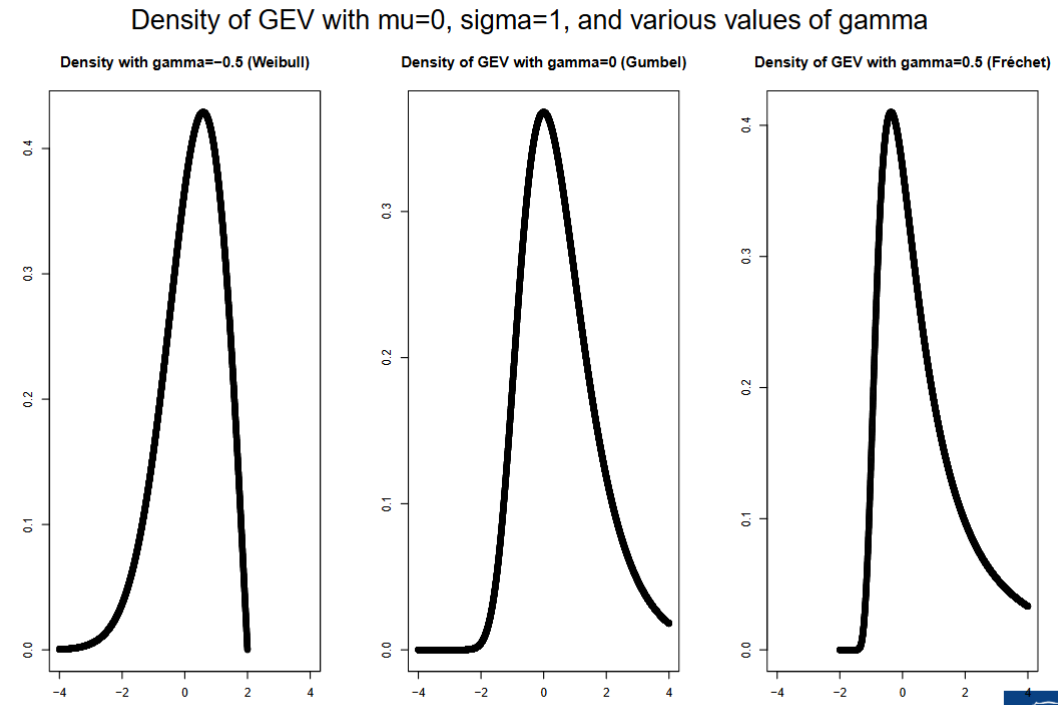
\includegraphics[width=0.6\linewidth]{Density of GEV Gamma.png}
\end{figure}

\subsubsection{Identifying a Fr\'echet GEV ($\gamma >$ 0)}
\begin{itemize}
    \item A function $L(x)$ is slowly varying at $\infty$ if
        $$\lim_{x\rightarrow\infty}\frac{L(tx)}{L(x)} = 1, \: \ t>0$$
    \item A function $h(x)$ is regularly varying at $\infty$ with index $\rho$ if
        $$\lim_{x\rightarrow\infty}\frac{h(tx)}{h(x)} = t^\rho \Leftrightarrow h(x) = x^\rho L(x), \: \ t > 0$$
\end{itemize}
\noi The limiting distribution of hte normalised maximum from an underlying df $F$ is of Fr\'echet type ($\gamma > 0$) if its survival function:
$$\tilde{F}(x) = 1 - F(x) = x^{\boldsymbol{-\frac{1}{\gamma}}}L(x)$$
\noi The rate of decay $\frac{1}{\gamma}$ is often known as the tail index of the distribution. We also know $\mathbb{E}[X^k] = \infty$ for $k > \frac{1}{\gamma}$. \\

\noi \textbf{Example: Pareto distribution}
\begin{align*}
    F(x) &= 1 - \Big( \frac{\theta}{\theta + x} \Big)^\alpha, \: \alpha >0, \theta > 0, x \geq 0 \\
    \tilde{F}(x) &= \Big(\frac{\theta}{\theta+x}\Big)^\alpha \\
    &= x^{-\alpha}\Big( \frac{\theta}{\frac{\theta}{x}+1} \Big)^{\alpha} \\
    &= x^{-\alpha}\Big( \frac{\theta x}{\theta + x} \Big)^\alpha = x^{-\alpha}L(x)
\end{align*}
\noi for $L(x) = \Big( \frac{\theta x}{\theta + x} \Big)^\alpha$, the rate of decay $\frac{1}{\gamma} = \alpha$, so the limiting distribution is of Fr\'echet type with $\gamma = \frac{1}{\alpha}$.

\subsubsection{Identifying a Gumbel GEV ($\gamma = 0$)}
\noi The limiting distribution of the normalised maximum from an underlying df $F$ is of Gumbel type ($\gamma = 0$) if it has finite moments of any positive order, i.e. $\mathbb{E}[X] < \infty$ for $k > 0$. Examples include Exponential, Normal, Gamma, Weibull, and Lognormal.

\subsubsection{Identifying a upper-bounded Weibull ($\gamma < 0$)}
\noi The limiting distribution of the normalised maximum from an underlying df $F$ is of upper-bounded Weibull type ($\gamma < 0$) if it has finite right end point (i.e. $x_F < \infty$) where the right endpoint is defined as $x_F = \sup\{x \in \mathbb{R}: F(x) < 1\}$.

\subsubsection{Estimation: Block Maxima (in R)}
\begin{itemize}
    \item The EVD is a distribution of maxima
    \item To fit we need a sample of maxima
    \item To achieve this, the data is transformed into \textbf{block maxima}
        \begin{enumerate}
            \item assume we have $n$ data points (\textit{say, monthly data over 1,000 years, so n=12,000})
            \item consider blocks of length $m$ (\textit{say, all observations in a given year such that m=12})
            \item the block maxima are then equal to the maximum observation within a block (\textit{the maximum value within each of the 1,000 years})
            \item we have then a sample size of $n/m$ (\textit{our sample size of maxima is of size 12000/12=1,000})
        \end{enumerate}
    \item The block maxima are then fitted to the EVD
    \item The larger the block size, the closer to the asymptotic distribution we get, but the less data we have (conflicting requirements)
    \item In R we use \texttt{fevd()} from package \texttt{extRemes}
\end{itemize} \phantom{i}

\noi \textbf{Example: with Data (in R)}: \\
\noi Consider three datasets with $n=12,000$, given in months, with columns named \texttt{beta} (simulated from beta), \texttt{gamm} (simulated from gamma), \texttt{logg} (simulated from log-gamma). \\

\noi Creating block maxima
\begin{lstlisting}
claims <- as_tibble(read_excel("simulated-claims.xlsx"))
# block maxima index
claims$block <- (claims$month - 1)%/%12 + 1
# %/% gives the integer part of the result of the division
blockmax <- tibble(betablock = aggregate(beta ~ block, claims,
max)$beta, gammblock = aggregate(gamm ~ block, claims, max)$gamm,
loggblock = aggregate(logg ~ block, claims, max)$logg)

# Can also plot the same for the gamma and log-gamma blocks
par(mfrow = c(1, 2))
plot(density(claims$beta), main = "Density of the beta claims",
xlab = "Claim amounts ($)", xlim = c(0, max(claims$beta)))
plot(density(blockmax$betablock),
main = "Density of the beta block maxima",
xlab = "Maximums over consecutive periods of 12 months ($)",
xlim = c(0, max(claims$beta)))

library(extRemes)
fit.beta <- fevd(blockmax$betablock)
fit.beta # shows parameter estiamtes, gamma < 0 
plot(fit.beta) # plots goodness of fit analysis

fit.gamm <- fevd(blockmax$gammblock)
fit.gamm # shows parameter estiamtes, gamma = 0 can be considered due to s.e.
plot(fit.gamm) # plots goodness of fit analysis

fit.logg <- fevd(blockmax$loggblock)
fit.logg # shows parameter estiamtes
plot(fit.logg) # plots goodness of fit analysis

# Example of plot(fit.beta)
\end{lstlisting}
\begin{figure}[H]
    \centering
    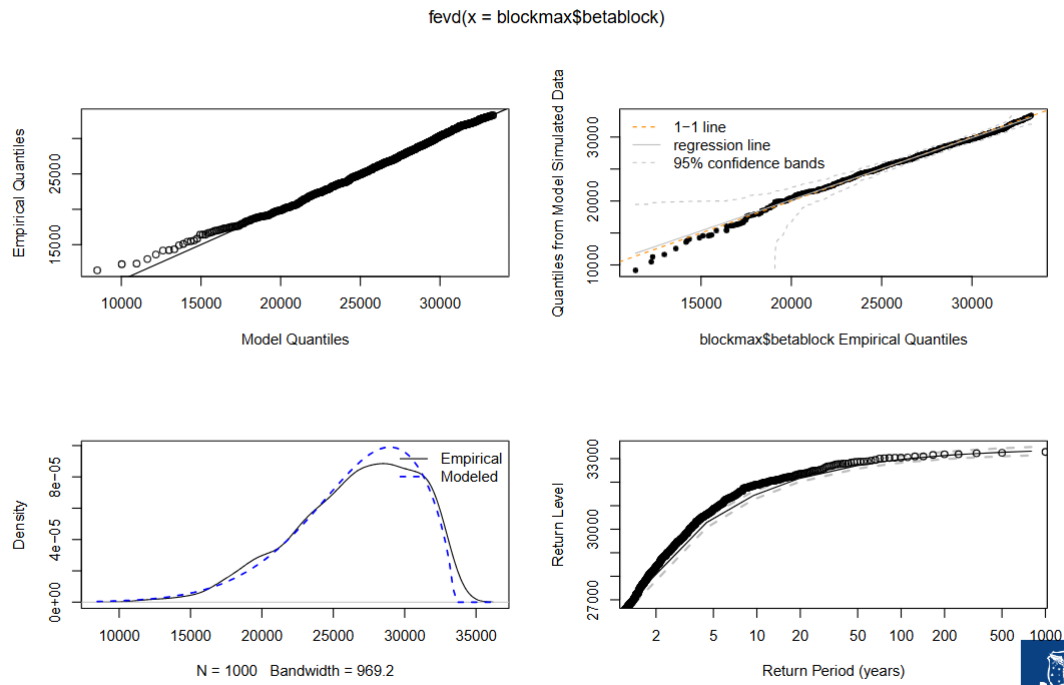
\includegraphics[width=0.9\linewidth]{block maxima diag plots beta.png}
\end{figure}
\begin{itemize}
    \item Top-left: if good fit dots should almost be a straight line,
    \item Top-right: black dates should fit to the fitted line,
    \item Bottom-left: depends on what the GEV looks like (beta gives upper-bounded weibull dist. and it is bounded around 33,000),
    \item Bottom-right: dots should closely follow line.
\end{itemize}

\subsection{GPD Distribution}
\begin{itemize}
    \item The tail is the distribution beyond a point. We characterise the tail with the df of the excess over threshold u (\textbf{threshold exceedance})
        $$F_u(x) = \Pr[Y - u \leq x | Y > u] = \frac{F(x+u) - F(u)}{1 - F(u)}, \ \ \ 0 \leq x < x_{F} - u$$
    \item For high $u$, $F_u(x)$, can be \textit{approximated} by a Generalised Pareto Distribution (GPD)
\end{itemize} \phantom{i}

$$G_{\gamma, \ \sigma}(x) = \begin{cases}
    1 - \Big( 1 + \gamma \frac{x}{\sigma} \Big)^{-\frac{1}{\gamma}} & \gamma \neq 0 \\
    1 - e^{-\frac{x}{\sigma}} & \gamma = 0
\end{cases}$$
\noi for a scale parameter $\sigma > 0$. \\

\noi We distinguish again three cases:
\begin{itemize}
    \item $\gamma < 0$ (upper bounded, also referred to as "Pareto Type II"): \textbf{light tail} $x \in (0, \sigma/|\gamma|)$
    \item $\gamma = 0$ (exponential): base case $x \in (0, \infty)$
    \item $\gamma > 0$ (Pareto): \textbf{heavy tail} $x \in (0, \infty)$
\end{itemize} \phantom{i}

\noi \textbf{Moments} \\
\noi The first central moments of $X$ (in excess of $u$) are
$$\mathbb{E}[X] = \frac{\sigma}{1-\gamma}, \: \gamma < 1$$
$$\text{Var}(X) = \frac{\sigma^2}{(1-\gamma)^2(1-2\gamma)}, \: \gamma < 1/2$$
\noi Note:
\begin{itemize}
    \item The first $k$ central moments exist only for $\gamma < 1/k$.
    \item $\mathbb{E}[X]$ is the stop loss premium (since $X$ is the excess over threshold $u$).
\end{itemize}

\subsubsection{Estimation: choice of threshold u (in R)}
\noi We seek to estimate the tail $\bar{F}(u+x) = \bar{F}(u)\bar{F}_u(x)$. To do this, we need to estimate:
\begin{itemize}
    \item Probability of exceeding u: $\widehat{\overline{F}(u)} = \frac{n_u}{n}$, which will be more accurate for $u$ not too large.
    \item Then for a given value of $u$: $\widehat{\overline{F}_u(x)} = \bar{G}_{\hat{\gamma}, \hat{\sigma}}(x)$, where $\hat{\gamma}(u)$ and $\hat{\sigma}(u)$ are estimated from the data in the tail above $u$ (via MLE). This approximation will work well only for large $u$.
\end{itemize} \phantom{i}

\noi The choice of $u$ presents conflicting requirements for $u$:
\begin{itemize}
    \item Larger $u$ will lead to a better approximation from a distributional perspective
    \item but larger $u$ reduces the amount of data to estimate $\bar{F}(u)$, $\gamma$ and $\sigma$
\end{itemize} \phantom{i}

\noi The choice is often also based on the following further considerations:
\begin{itemize}
    \item mean-excess plot: the slope should have the same sign as $\gamma$
    \item log-log plot: linear for heavy tails
    \item stability of $\hat{\gamma}$ for different choices of $u$
    \item Hill plot: stability of Hill estimator $\hat{\alpha}$
    \item goodness of fit for different choices of $u$
\end{itemize} \phantom{i}

\noi \textbf{Example: SUVA dataset data} \\
\noi Size of tail (want to choose threshold which is about $5\%$ of values above threshold, e.g. $5000$ in this example):
\begin{lstlisting}
numbexc <- c()
for (i in 250:20000) {
    numbexc <- c(numbexc, length(SUVA$medcosts[SUVA$medcosts > i]))
}

par(mfrow=c(1,2))
plot(250:20000, numbexc, xlab = "Threshold", ylab = "Number of claims exceeding the threshold",
    col="darkblue", bg="lightblue", pch=21)
plot(250:20000, numbexc/length(SUVA$medcosts), xlab = "Threshold", ylab = "Proportion of claims
    above threshold", col = "darkblue", bg = "lightblue", pch = 21)
\end{lstlisting}
\begin{figure}[H]
    \centering
    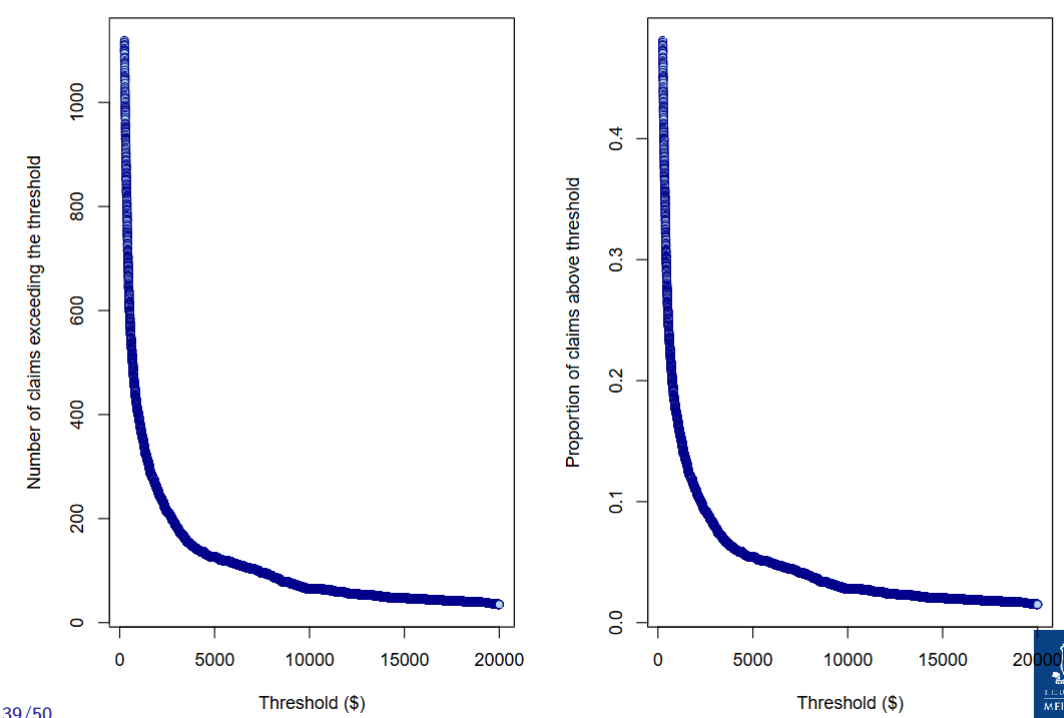
\includegraphics[width=0.7\linewidth]{GPD - example - size of tail.png}
\end{figure}

\noi Mean-excess plot (if upwards sloping means heavy tail so $\gamma > 0$, if downwards sloping means lighter tail so $\gamma < 0$):
\begin{lstlisting}
extRemes::mrlplot(SUVA$medcosts, xlim = c(250, 20000))
\end{lstlisting}
\begin{figure}[H]
    \centering
    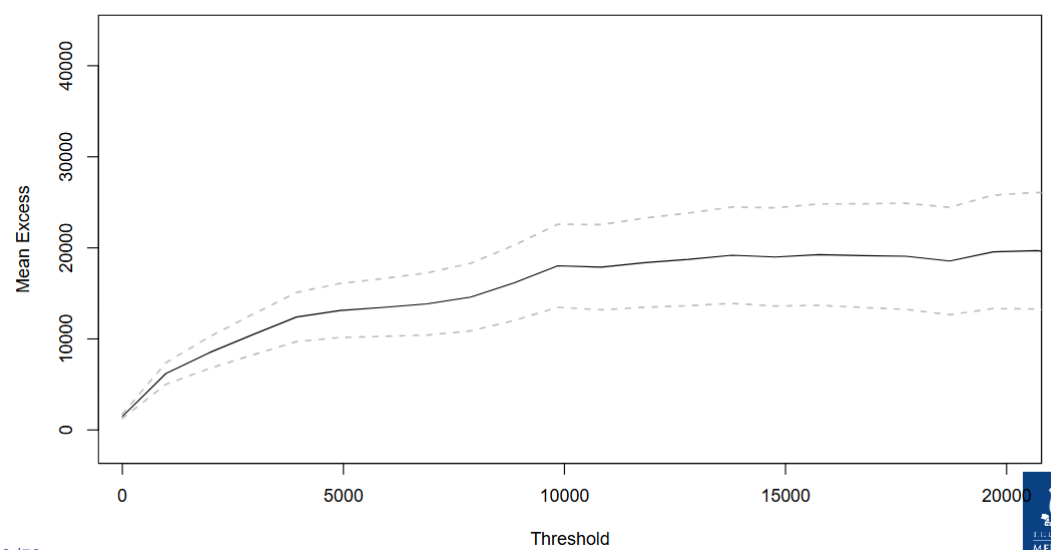
\includegraphics[width=0.7\linewidth]{GPD - example - mean excess plot.png}
\end{figure}

\noi Empirical $\bar{F}$ on log-log scale:
\begin{lstlisting}
evir::emplot(SUVA$medcosts, alog = "xy", labels = TRUE)
\end{lstlisting}
\begin{figure}[H]
    \centering
    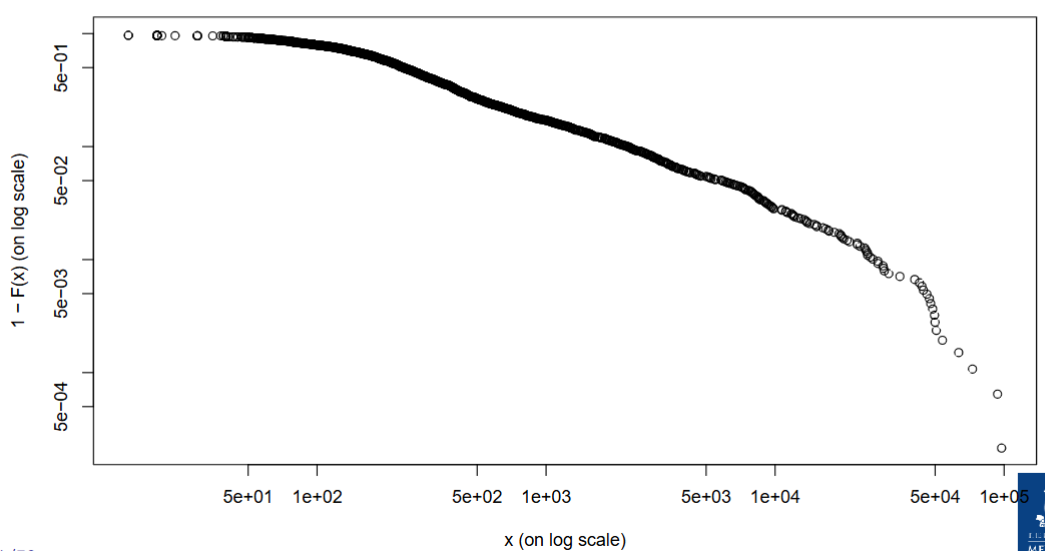
\includegraphics[width=0.7\linewidth]{GPD - example - empirical log-log.png}
\end{figure}
\noi good potential candidate for threshold is a bit before $5000$, before line goes funny \\

\noi Stability of $\hat{\gamma}$, only bottom graph is important (top concerns the scale $\sigma$ so ignore), need to find an area where the plot is flat then that is a good threshold value and the y-axis indicates the $\gamma$:
\begin{lstlisting}
extRemes::threshrange.plot(SUVA$medcosts, r = c(250, 20000), nint = 80)
\end{lstlisting}
\begin{figure}[H]
    \centering
    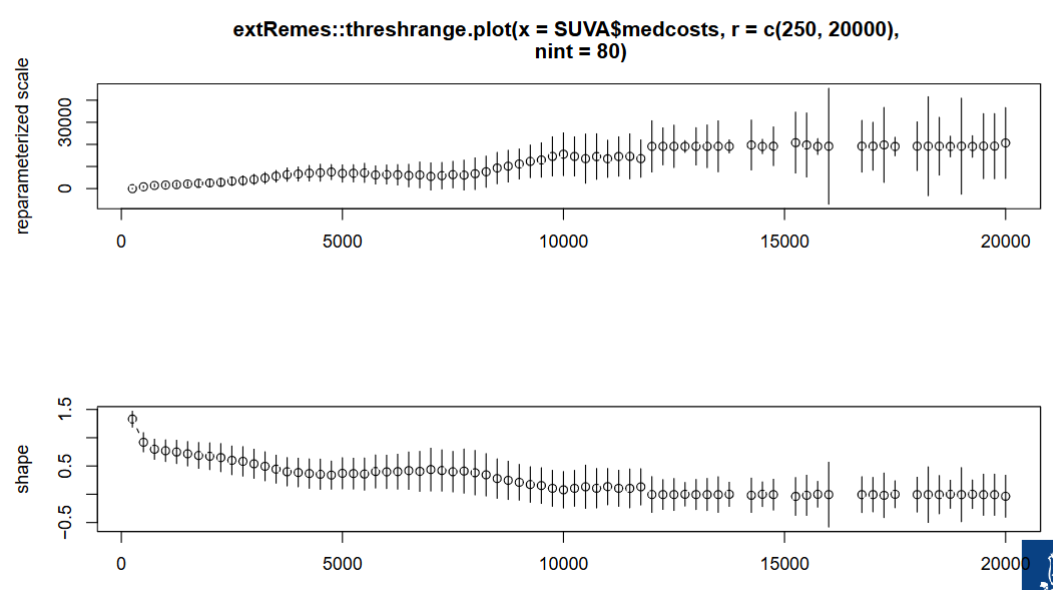
\includegraphics[width=0.7\linewidth]{GPD - example - stability of gamma.png}
\end{figure}

\noi Hill plot, Stabaility of $\hat{\gamma}$ is more important than this, if need to just look at where it is flat just before it shoots up on the left:
\begin{lstlisting}
evir::hill(SUVA$medcosts) # note that alpha is inverse of gamma
\end{lstlisting}
\begin{figure}[H]
    \centering
    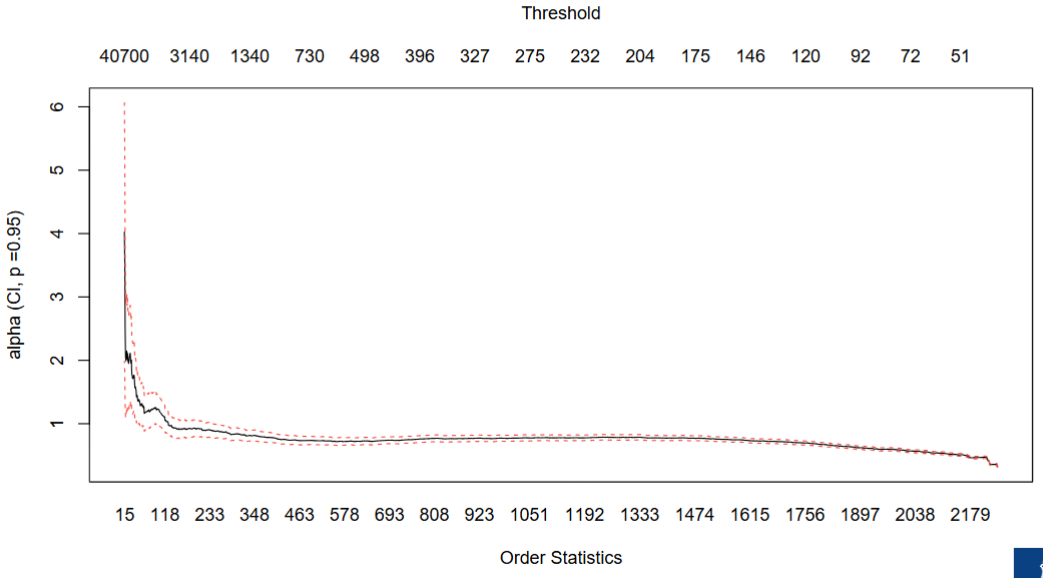
\includegraphics[width=0.7\linewidth]{GPD - example - hill plot.png}
\end{figure}

\noi Estimation results for $u=500$
\begin{lstlisting}
fit.SUVA.500 <- fevd(SUVA$medcosts, threshold = 500, type = "GP",
time.units = "1/year")
fit.SUVA.500 # shows estimated parameters of shape and scale
numbexc[501 - 250] # n_u (noting that numbexc[1] = n_250)
## 616
plot(fit.SUVA.500) # top 2 graphs show its bad choice
\end{lstlisting}
\begin{figure}[H]
    \centering
    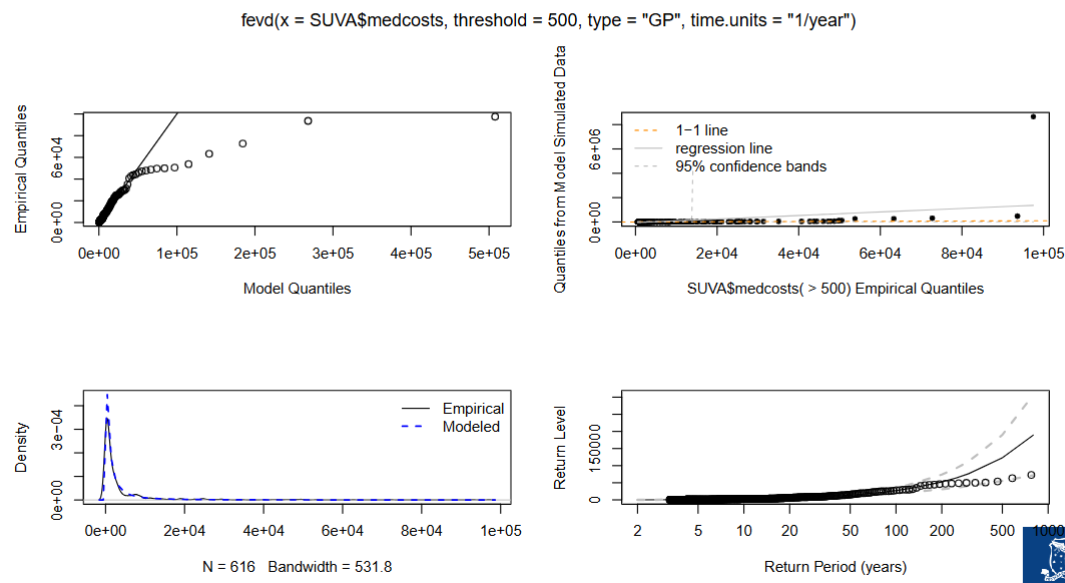
\includegraphics[width=0.7\linewidth]{GPD - example - u500.png}
\end{figure}

\noi Estimation results for $u=5500$
\begin{lstlisting}
fit.SUVA.5500 <- fevd(SUVA$medcosts, threshold = 5500, type = "GP",
time.units = "1/year")
fit.SUVA.5500 # shows estimated parameters of shape and scale
numbexc[5501 - 250] # n_u
## 118
plot(fit.SUVA.5500) # top 2 graphs show its bad choice
\end{lstlisting}
\begin{figure}[H]
    \centering
    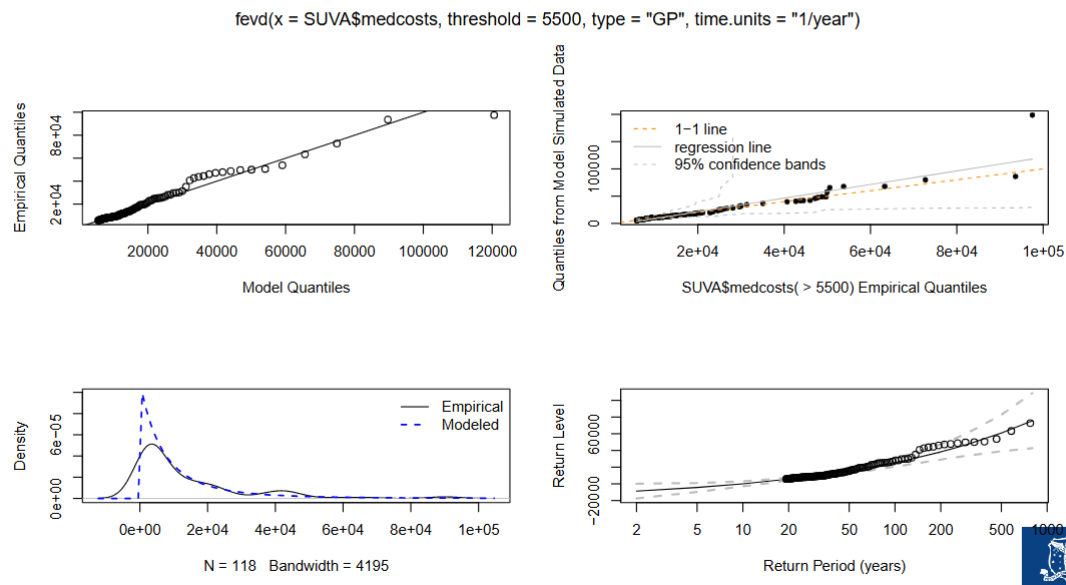
\includegraphics[width=0.7\linewidth]{GPD - example - u5500.png}
\end{figure}

\noi Estimation results for $u=9500$
\begin{lstlisting}
fit.SUVA.9500 <- fevd(SUVA$medcosts, threshold = 9500, type = "GP",
time.units = "1/year")
fit.SUVA.9500 # shows estimated parameters of shape and scale
numbexc[9501 - 250] # n_u
## 70
plot(fit.SUVA.9500) # top 2 graphs show its bad choice
\end{lstlisting}
\begin{figure}[H]
    \centering
    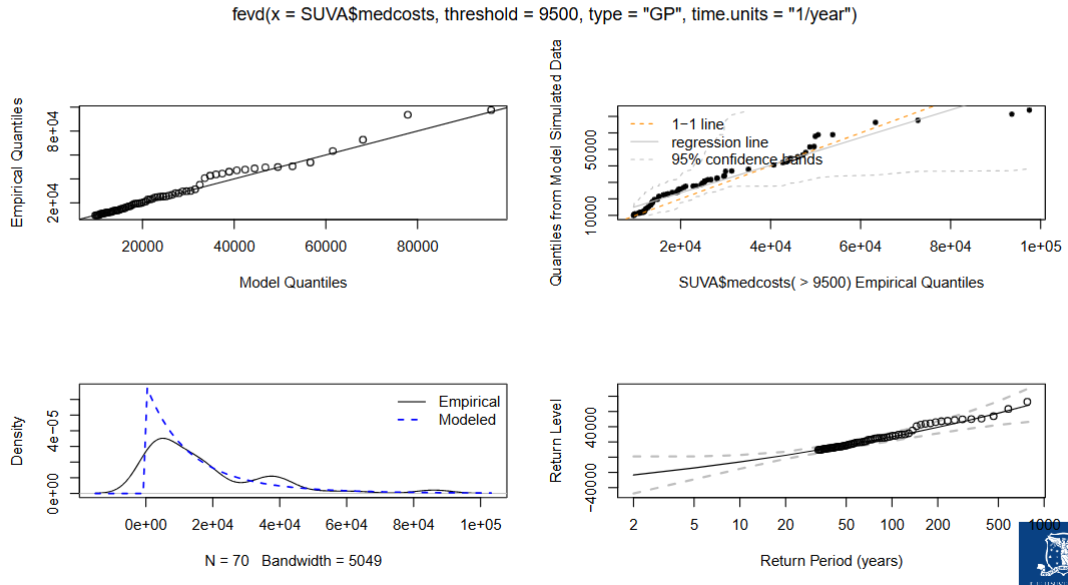
\includegraphics[width=0.7\linewidth]{GPD - example - u9500.png}
\end{figure}

\noi Return level in R:
\begin{lstlisting}
library(extRemes)

# Example data: say "data" is your numeric vector of observations
fit <- fevd(data, threshold = u, type = "GP")
return.level(fit, return.period = T)
# T = return period, e.g. 100 for 100 year return
\end{lstlisting}
\noi The return level is the value you expect to occur once in every $T$ periods (where $T$ is the return period, e.g. $T = 100$ years). \\

\noi QQ Plot of fit (just QQ byitself):
\begin{lstlisting}
# QQ Plot
plot(fit, type="qq", main="GPD QQ-plot: empirical vs theoretical")
abline(0,1, lty="dashed", col="blue")
\end{lstlisting}

\newpage
%%%%%%%%%%%%%%%%%%%%%%%%%%%%%%%%%%%%%%%%%%%%%%%%%%%%%%%%%%%%%%%%%%%%%%%%%%%%%%
\section{Module 7 – Time Series Fundamentals}
\subsection{Preliminaries and White Noise Basics}
\noindent A time series is a sequence of rv's $x_1, x_2, x_3,...$, denoted $\{x_t\}$. \textbf{White Noise}: $w_t$ is uncorrelated (over $t$) with mean $0$ and finite variance $\sigma_w^2$, it can be $iid$ and Gaussian, or just $iid$. \\

\noindent Plot a gaussian white noise series with a 3-point moving average ($v_t = \frac{1}{3}(w_{t-1}+w_t+w_{t+1})$):
\begin{lstlisting}
w = rnorm(500, 0, 1) # 500 N(0,1) variates
plot.ts(w, ylim=c(-3,3), main="white noise")
v = stats::filter(w, sides=2, filter=rep(1/3,3)) # moving average
plot.ts(v, ylim=c(-3,3), main="moving average)
\end{lstlisting}

\noindent Plot an auto-regression with gaussian white noise $x_t = x_{t-1}-0.9x_{t-2}+w_t$ for $t=1,...,500$. We also need $2$ initial conditions since the time series goes $2$ periods back (to avoid this problem we run the AR for longer than needed to avoid this issue and remove first $50$ observations).
\begin{lstlisting}
w = rnorm(550, 0, 1)
x = stats::filter(w, filter = c(1, -0.9), method="recursive")[-(1:50)] # remove first 50
plot.ts(x, ylab="autoregression", main=expression(x[t] == x[t-1] - 0.9 * x[t-2] + w[t]))
\end{lstlisting}

\noindent \textbf{Notes of R}: \texttt{filter(x, filter, method = c("convolution), sides=2)}
\begin{itemize}
    \item \texttt{filter}: vector of weights (in reverse time order),
    \item \texttt{method}: default is "convolution" (for MA) and "recursive" (for AR),
    \item \texttt{sides}: $1$ for past values only, and $2$ if weights are centred around lag $0$.
\end{itemize}

\subsubsection*{Random walk with drift}
\noi The random walk with drift looks back only one time unit:
$$x_t = \delta + x_{t-1} + w_t = \delta t + \sum_{j=1}^{t}{w_j} \text{, initial condition } x_0 = 0$$
\begin{itemize}
    \item If $\delta = 0$ then it is a random walk
    \item $\Delta x_t = x_{t+1} - x_t = w_{t+1}$ so only depends on random noise and nothing prior
    \item $\mu_{x_t} = \mathbb{E}[x_t] = \delta t$ and $\text{Var}(x_t) = t \sigma_w^2$, so mean and variance varies with time
    \item $\gamma_x(s,t) = \text{Cov}(\sum_{j=1}^s{w_j}, \sum_{k=1}^{t}w_k) = \text{min}\{s,t\}\sigma_w^2$
\end{itemize}

\subsubsection{Auto-covariance and correlation functions}
\noi \textbf{Auto-covariance function}:
$$\gamma_x(s, t) = \text{Cov}(x_s, x_t) = \mathbb{E}[(x_s - \mu_{x_s})(x_t - \mu_{x_t})]$$
\noi A smooth series $\rightarrow$ large $\gamma$ even for large lag, for choppy series $\rightarrow$ $\gamma$ is nearly $0$ for large lags. \\

\noi \textbf{Cross-covariance function}:
$$\gamma_{xy}(s, t) = \text{Cov}(x_s, y_t) = \mathbb{E}[(x_s - \mu_{x_s})(y_t - \mu_{y_t})]$$

\noi \textbf{Useful Covariance Property}: \\
\noi If $U = \sum_{j=1}^m{a_jX_j}$ and $V = \sum_{k=1}^r{b_kY_k}$, then:
$$\text{Cov}(U, V) = \sum_{j=1}^{m}{\sum_{k=1}^{r}}{a_jb_k\text{Cov}(X_j, Y_k)}$$

\noi \textbf{Auto-correlation function}:
$$-1 \leq \rho(s,t) = \frac{\gamma(s,t)}{\sqrt{\gamma(s,s)\gamma(t,t)}} \leq 1$$
\noi Measurers the \textit{linear} predictability of the series at time $t$, say $x_t$, using only the value of $x_s$. \\

\noi \textbf{Cross-correlation function}:
$$-1 \leq \rho_{xy}(s,t) = \frac{\gamma_{xy}(s,t)}{\sqrt{\gamma_{x}(s,s)\gamma_y(t,t)}} \leq 1$$


\subsection{Stationarity}
\subsubsection{Strictly Stationary}
\noindent A time series which the probabilistic behaviour of every collection of values $\{x_{t_1}, ..., x_{t_k}\}$ is identical to that of the time shifted (for any $h$) $\{x_{t_1+h},...,x_{t_k+h}\}$. That is:
$$\mathbb{P}(x_{t_1} \leq c_1, ..., x_{t_k} \leq c_k) = \mathbb{P}(x_{t_1+h} \leq c_1,...,x_{t_k+h} \leq c_k)$$
\noindent For all $k=1,2,...$, all the time points $t_i$, numbers $c_i$ and \textbf{all time shifts} $h=0, \pm 1, \pm2,...$ This implies:
\begin{itemize}
    \item Identical marginals of dimensions $< k$ for any shift $h$
    \item Constant mean: $\mu_{xs} = \mu_{xt} \equiv \mu$
    \item The auto-covariance function depends only on lag $t-s$: $\gamma(s,t) = \gamma(s+h, t+h)$
    \item A weakly stationary Gaussian time series is also strictly stationary.
\end{itemize}

\subsubsection{Weak Stationary}
\noindent Time series is weakly stationary when it is a finite variance process such that:
\begin{enumerate}
    \item The mean value function, $\mu_{xt}$ is \textbf{constant} and does not depend on time $t$, and
    \item The auto-covariance function, $\gamma(s,t)$ depends on $s$ and $t$ \textbf{only through their difference} $|s-t|$.
\end{enumerate}

\subsubsection{Properties}
\begin{itemize}
    \item By condition 1 (constant mean): $\mu_t = \mu$
    \item By condition 2 (covariance only depends on lag): $\gamma(t+h, t) = \textbf{Cov}\boldsymbol{(x_{t+h}, x_t)} = \text{Cov}(x_h, x_0) = \gamma(h,0) \equiv \boldsymbol{\gamma(h)} = \mathbb{E}[(x_{t+h} - \mu)(x_t - \mu)]$
    \item $\gamma(h)$ is non-negative definite: $0 \leq \text{Var}(a_1x_1 + ... + a_nx_n) = \sum_{j=1}^n{\sum_{j=1}^{n}{a_ja_k\gamma(j-k)}}$
    \item Also, $|\gamma(h)| \leq \gamma(0)$ and $\gamma(h) = \gamma(-h)$
    \item The ACF of the stationary time series becomes: $-1 \leq \boldsymbol{\rho(h)} = \frac{\gamma(t+h,t)}{\sqrt{\gamma(t+h, t+h)}\gamma(t,t)} = \boldsymbol{\frac{\gamma(h)}{\gamma(0)}} \leq 1$.
\end{itemize}

\subsubsection*{Examples of (non)-stationarity}
\noindent \textbf{Stationary white noise}: \\
\noindent We have $\mu_{w_t} = 0$ and $\gamma_w(h) = \text{Cov}(w_{t+h}, w_t) = \begin{cases}
    \sigma_w^2 & h=0, \\ 0 & h \neq 0
\end{cases}$, \\
\noindent These are both independent of time. Hence, the white noise satisfies both conditions and is (weakly) stationary. Furthermore, $\rho_w(h) = \begin{cases}
    1 & h=0, \\ 0 & h \neq 0.
\end{cases}$ \\
\noindent If in addition $w_t \sim \text{iid} \textbf{N}(0, \sigma_w^2)$, then it is also strictly stationary. \\

\noindent \textbf{Stationary moving average: for 3-point MA} we have \\
\noindent $\mu_{v_t} = 0$ and $\gamma_v(h) = \begin{cases}
    \frac{3}{9}\sigma_w^2 & h=0, \\ \frac{2}{9}\sigma_w^2 & h = \pm 1, \\ \frac{1}{9}\sigma_w^2 & h=\pm 2, \\ 0 & |h| >2
\end{cases}$ \\
\noindent Which are both independent of time. Hence, the 3-point MA satisfies both conditions and is stationary. Furthermore the ACF is symmetric around lag 0. \\

\noindent \textbf{Non-stationary random walk}: for the random walk model $x_t = \delta t + \sum_{j=1}^t{w_j}$ we have, \\
$$\mu_{x_t} = \delta t \text{ and } \gamma(s,t) = \text{min}\{s,t\}\sigma_w^2$$
\noindent The mean depends on time $t$ and the auto covariance function depends on $s$ and $t$ (not just their difference), so the random walk is NOT stationary. \\
\noindent Furthermore, Var$(x_t) = \gamma_x(t,t) = t\sigma_w^2$ which increases without bound as $t \rightarrow \infty$.

\subsubsection{Trend Stationarity}
\begin{itemize}
    \item If the second condition (on the ACF that it only depends on lag) is satisfied, but not the first condition (on the mean being constant and independent of time), we have Trend Stationarity.
    \item The model has a stationary behaviour around its trend.
\end{itemize} \phantom{i}
\noindent Example: if $x_t = \alpha + \beta t + y_t$ (assuming $y_t$ is stationary):
$$\mu_{x,t} = \mathbb{E}[x_t] = \alpha + \beta t + \mu_y \text{ and } \gamma_x(h) = \gamma_y(h)$$
\noindent Therefore the mean is \textit{not} independent of time and the auto-covariance function is independent of time.

\subsubsection{Joint Stationarity}
\noindent Two time series $x_t$ and $y_t$ are jointly stationary if they are each stationary AND the cross covariance function is a function of only lag $h$.
$$\gamma_{xy}(h) = \text{Cov}(x_{t+h},y_t) = \mathbb{E}[(x_{t+h} - \mu_x)(y_t - \mu_y)] \text{ and } 1 \leq \rho_{xy}(h) = \frac{\gamma_{xy}(h)}{\sqrt{\gamma_x(0)\gamma_y(0)}} \leq 1$$
\noindent They aren't symmetric around zero. However, we have $\gamma_{xy}(h) = \gamma_{yx}(-h)$ and $\rho_{xy}(h) = \rho_{yx}(-h)$. \\

\noindent \textbf{Example of joint stationarity}, consider $x_t = w_t + w_{t-1}$ and $y_t = w_t - w_{t-1}$, we know then:
\begin{align*}
    \gamma_x(0) &= \gamma_y(0) = 2\sigma_w^2 \\
    \gamma_x(-1) &= \gamma_x(1) = \sigma_w^2 \\
    \gamma_y(-1) &= \gamma_y(1) = -\sigma_w^2
\end{align*} \phantom{i}
\noindent and
$$\gamma_{xy}(-1) = -\sigma_w^2, \: \gamma_{xy}(0) = 0, \: \text{ and } \gamma_{xy}(1) = \sigma_w^2$$
\noindent so that:
\begin{align*}
    \rho_{xy}(h) = \begin{cases}
        0 & h=0, \\
        1/2 & h=1, \\
        -1/2 & h=-1, \\
        0 & |h| \geq 2
    \end{cases}
\end{align*} \phantom{i}
Which depends only on the lag $h$, so both series are jointly stationary.

\subsubsection{Linear processes}
\noi A \textit{linear process}, $x_t$, is defined to be a linear combination of white noise variates, and is given by:
$$x_t = \mu + \sum_{j=-\infty}^{\infty}{\Psi_j w_{t-j}}, \: \sum_{j=-\infty}^{\infty}|\Psi_j| < \infty$$
\noi \textbf{Properties}:
\begin{itemize}
    \item The auto-covariance is given by: $\gamma_x(h) = \sigma_w^2\sum_{j=-\infty}^{\infty}{\Psi_{j+h}\Psi_j}$ for $h \geq 0$
    \item It has finite variance if $\sum_{j=-\infty}^{\infty}{\Psi_j^2} < \infty$
    \item $x_t$ depends on the future (if $j<0$), the present (if $j=0$), and the past (if $j > 0$)
    \item If a process does NOT depend on the future it is \textbf{casual}: $\Psi_j = 0$ for $j < 0$
\end{itemize}

\subsection{Estimation of Correlation}
\subsubsection{Sample mean}
\noi Assuming that a time series is stationary the mean function $\mu_t = \mu$ is constant so that we can estimate it by the sample mean:
$$\bar{x} = \frac{1}{n}\sum_{t=1}^n{x_t}$$
\noi This estimator is unbiased, $\mathbb{E}[\bar x] = \mu$ and has the standard error of: $\text{Var}(\bar x) = \frac{1}{n^2}\text{Cov}(\sum_{t=1}^n{x_t}, \sum_{s=1}^n{x_s}) = \frac{1}{n}\sum_{h=-n}^n{(1-\frac{|h|}{n})}\gamma_x(h)$

\subsubsection{Sample autocovariance function}
$$\hat \gamma(h) = \frac{1}{n}\sum_{t=1}^{n-h}{(x_{t+h} - \bar x)(x_t - \bar x)} \text{ with } \hat \gamma(-h) = \hat \gamma(h) \text{ for } h=0,1,...,n-1$$
\begin{itemize}
    \item The estimator is unbiased
    \item The sum is bounded to $n-h$ because $x_{t+h}$ is not available for $t+h >n$
\end{itemize}
\subsubsection{Sample auto-correlation function}
$$\hat \rho(h) = \frac{\hat \gamma(h)}{\hat \gamma(0)}$$
\noi Under certain conditions, if $x_t$ is white noise, then for large $n$, the SACF is approximately normally distributed with $\mu=0$ and $\sigma_{\hat \rho(h)} = \frac{1}{\sqrt{n}}$ \\

\noi \textbf{Testing for significance of auto-correlation} \\
\noi We can test whether lagged observations are uncorrelated (which is a requirement for white noise):
\begin{itemize}
    \item Test for significance of the $\hat \rho$'s at different lags: check how many $\hat \rho$ values lie outside of the interval $\pm2/\sqrt n$ (a $95\%$ C.I.)
    \item Should expect approximately \textbf{1 out of 20} to lie outside the interval if the sequence is white noise, many more would invalidate the whiteness assumption
    \item The R function \texttt{acf} automatically displays those bounds with dashed blue lines
\end{itemize} \phantom{i}

\noi \textbf{Example with SOI data}
\begin{lstlisting}
acf(soi, main="Sample Auto-correlation function of SOI")
r <- round(acf(soi, 6, plot=FALSE)$acf[-1], 3) # first 6 sample acf
# The series is clearly NOT white noise as lots of lines beyond dashed line

# Visualising dependence of SOI pairs with 6 month lag
plot(stats::lag(soi, -6), soi, main="SOI pairs of values 6 months apart")
legend("topleft", legend = r[6])
\end{lstlisting}

\subsubsection{Sample cross-covariances and cross-correlations}
\noi \textbf{Sample cross-covariance function}
$$\hat \gamma_{xy}(h) = \frac{1}{n}\sum_{t=1}^{n-h}{(x_{t+h} - \bar x)(y_t - \bar y)}$$
\noi where $\hat \gamma_{xy}(-h) = \hat \gamma_{xy} = h$ determines the function for \texit{negative} lags \\

\noi \textbf{Sample cross-correlation function}
$$-1 \leq \hat \rho_{xy}(h) = \frac{\hat \gamma_{xy}(h)}{\sqrt{\hat \gamma_{x}(0) \hat \gamma_y(0)}} \leq 1$$
\noi \textit{Note}: graphical examinations of this function provide information about the leading or lagging relations in the data as shown below.

\subsubsection{Prediction using cross-correlation}
\noi A lagging relation between two series $x_t$ and $y_t$ may be exploted for predictions. For instance if
$$y_t = Ax_{t - \ell} + w_t$$
\noi $x_t$ is said to \textbf{lead} $y_t$ for $\ell > 0$, and is said to \textbf{lag} $y_t$ for $\ell < 0$. \\

\noi If the relation above holds true, then the lag $\ell$ can be inferred form the cross-covariance of $y_{t+h}$ on $x_t$ denoted $\gamma_{yx}(h)$:
\begin{itemize}
    \item If $w_t$ is uncorrelated with $x_t$ then, $\gamma_{yx}(h) = \text{Cov}(y_{t+h}, x_t) = A \gamma_{x}(h - \ell)$
    \item We know $|\gamma_x(h - \ell)| \leq \gamma_x(0)$, and so $\ell$ = h is the peak of $\gamma_{yx}(h)$. Also $h = \ell$ will be positive if $x_t$ leads $y_t$ or negative if $x_t$ lags $y_t$
    \item Done using \texttt{ccf} in R
\end{itemize} \phantom{i}

\noi \textbf{SOI and Recruitment correlation analysis}
\begin{lstlisting}
ccf(rec, soi, 48, main = "SOI vs recruitment, ylab = "CCF") # so y = rec and x = soi
# The plot has a peak at h=6, suggesting SOI leads recruitment by 6 months
\end{lstlisting}
\newpage
%%%%%%%%%%%%%%%%%%%%%%%%%%%%%%%%%%%%%%%%%%%%%%%%%%%%%%%%%%%%%%%%%%%%%%%%%%%%%%%%%
\section{Module 8 - Time Series Smoothing and Exploratory Analysis}

\subsection{Regression in time series context}
\noi Assume that some dependent time series $x_t$, can be make up of a collection of $q$ independent time series $z_{t1},z_{t2},...,z_{tq}$ where we first regard the inputs as fixed and known. Therefore we have:
$$x_t = \beta_0 + \beta_1z_{t1} + \beta_2z_{t2} + ... + \beta_qz_{tq} + w_t$$

\noi \textbf{Example regression with time variable} \\
\noi The monthly price $x_t$ of a chicken in the US, we model the \textit{trend} with a linear regression: $x_t = \beta_0 + \beta_1 t + w_t$, where $z_t$ are months in the data ($q=1$), we also assume that the $w_t$ are iid gaussian white noise (which may not be true in reality.
\begin{lstlisting}
summary(fit <- lm(chicken~time(chicken), na.action=NULL))
# Estimate Std.Error t.value
# (Intercept) -7131.02 162.41 -43.9
# time(chicken) 3.59 0.08 44.4
# --
# Residual standard error: 4.7 on 178 degrees of freedom

# Note that beta hat 1 = 3.59 meaning an increase of about 3.6 cents per year with
# a standard error of 0.081

plot(chicken, ylab="cents per pound")
abline(fit) # add the fitted line
\end{lstlisting}

\noi \textbf{Example regression with lagged variables} \\
\noi Previously we found that SOI leads Recruitment by six months. The relationship is not exactly linear by we consider $R_t = \beta_0 + \beta_1 S_{t-6} + w_t$. Under fitting from the following R code we get $\hat R_t = 65.790 - 44.283_{(2.781)}S_{t-6}$
\begin{lstlisting}
fish = ts.intersect(rec, soiL6=lag(soi,-6), dframe=TRUE) # to match up lagged timings
summary(fit1 <- lm(rec~soiL6, data=fish, na.action=NULL))
# Estimate Std.Error t.value Pr(>|t|)
# (Intercept) 65.790 1.088 60.47 <2e-16 ***
# time(chicken) -44.283 2.781 -15.92 <2e-16 ***
# The low p-values imply that SOI is a strong predictor of recruitment

# The same output without ts.intersect can be done via:
library(dynlm)
summary(fit2 <- dynlm(rec ~ L(soi, 6)))
\end{lstlisting}

\subsubsection{De-trending via regression and differencing}
\noi \textbf{Context} \\
\noi $x_t = \mu_t + y_t$ is called \textit{trend stationary} if $y_t$ is stationary. \\

\noi "Removing" $\mu_t$ is called \textbf{de-trending}, and there are two types:
\begin{enumerate}
    \item via regression: fitting a regression model for $\hat \mu_t$ (parametric)
    \item via differencing: modifying the series by looking at differences over time, rather than absolute values (non-parametric)
        \begin{itemize}
            \item Good if $\mu_t$ does not look like a linear trend
            \item $\nabla x_t \equiv x_t - x_{t-1}$
            \item Differencing $n$ times ($\nabla^n$) removes a polynomial trend of degree $n$
        \end{itemize}
    \item \textit{Note}: Differencing is always at least as good as regression when it comes to de-trending
\end{enumerate} \phantom{i}

\noi \textbf{Example: Chicken prices de-trended via regression}
\begin{lstlisting}
fit <- lm(chicken ~ time(chicken), na.action=NULL)
plot(resid(fit), type="l", main = "Price of chicken de-trended via regression")
# lots outside CI bands so not reasonably white noise
\end{lstlisting}
\noi Note that the residuals are $x_t - \hat \mu_t = y_t$ which we would like to be stationary. \\

\noi \textbf{Example: Global temperature de-trended via differencing}
\begin{lstlisting}
plot(gtemp_land, type="o") # Clear upward somewhat linear trend
plot(diff(gtemp_land), type="l", main="Global temps de-trended via differencing")
acf(diff(gtemp_land), 48) # only 2 in 48 outside of CI bands so reasonably white noise
\end{lstlisting}

\subsection{Scatter plot matrices to visualise relationships}
\noi \textbf{Transformations}: \\
\noi If obvious non-linear behaviour, can lead to non-stationarity, and transformations may be useful to \textit{equalise} the variability like $y_t = \log(x_t)$. \\

\noi \textbf{Scatter plot matrices}: \\
\begin{itemize}
    \item A preliminary data processing technique, to visualise the relations between series at different lags.
    \item Scatter plots (one for each lag) are informative to diagnose \textbf{non-linear} relationships (unlike ACF which focuses on linear predictability only).
    \item They give a visual sense of which lag will lead to the best predictability
    \item The red lines are \textit{locally weighted scatter plot smoothing} (lowess) lines -- they help identify non-linear relationships.
\end{itemize} \phantom{i}

\noi \textbf{Example: SOI and SOI vs Recruitment}
\begin{lstlisting}
lag1.plot(soi, 12) # red lines are more or less linear for lagged SOI so sample ACF is meaningful
lag2.plot(soi, rec, 8) # red lines are highly nonlinear around lags 5-8
\end{lstlisting}

\noi Using dummy variables we can model this (where $D_t = 0$ if $S < 0$ ($1$ otherwise)).
\begin{align*}
    R_t &= \beta_0 + \beta_1 S_{t-6} + \beta_2D_{t-6} + \beta_3D_{t-6}S_{t-6} + w_t \\
    &= \begin{cases}
        \beta_0 + \beta_1 S_{t-6} + w_t & \text{if  } S_{t-6} < 0, \\
        (\beta_0 + \beta_2) + (\beta_1 + \beta_3)S_{t-6} + w_t & \text{if  } S_{t-6} \geq 0
    \end{cases}
\end{align*}
\begin{lstlisting}
dummy = ifelse(soi < 0, 0, 1) # for piecewise regression
fish = ts.intersect(rec, soiL6 = stats::lag(soi, -6), dL6 = stats::lag(dummy, -6), dframe=TRUE)
summary(fit <- lm(rec ~ soiL6 * dL6, data = fish, na.action=NULL))
# Coefficients:
# Estimate Std.Error t.value
# (Intercept) 74.479 2.865 25.998
# soiL6 -15.358 7.401 -2.075
# dL6 -1.139 3.711 -0.307
# soiL6:dL6 -51.244 9.523 -5.381
# ---
# Residual standard error: 21.84 on 443 degrees of freedom
# Multiple R-squared: 0.4024
# F-statistic: 99.43 on 3 and 443 DF
attach(fish)
plot(soiL6, rec)
lines(lowess(soiL6, rec), col=4, lwd=2)
points(soiL6, fitted(fit), pch='+', col=2)
plot(resid(fit))
acf(resid(fit)) # not white noise still since lots outside of CI, need to model cycles
\end{lstlisting}

\subsection{Types of Smoothers (MA, Kernel, Lowess, and Splines)}
\subsubsection*{Moving Average Smoothing}
\noi If $x_t$ represents the observations, then
$$m_t = \sum_{j=-k}^{k}{a_jx_j} \text{ where, } a_j = a_{-j} \geq 0 \text{, and } \sum_{j=-k}^{k}a_j = 1$$
\noi is a symmetric (two-sided) moving average of the data \\

\noi \textbf{Example: Moving Average Smoother on SOI}
\begin{lstlisting}
wgts <- c(0.5, rep(1, 11), 0.5)/12 # sums to 1
soif <- stats::filter(soi, sides = 2, filter = wgts)
par()
plot(soi, main="MA smoother of SOI")
lines(soif, lwd = 3, col = "blue")

# To show visually the box-car shape of the weights
par(fig = c(.65, 1, .65, 1), new = TRUE)
nwgts = c(rep(0,20), wgts, rep(0,20))
plot(nwgts, type="l", ylim = c(-.02,.1), xaxt='n', yaxt='n', ann=FALSE)
\end{lstlisting}
\begin{itemize}
    \item This method removes (filters out) the obvious annual temperature cycles, and helps visualise the El Nino cycles
    \item However, it is still quite choppy, probably due to the (relatively non smooth) "boxcar" weights
\end{itemize}

\subsubsection*{Kernel Smoothing}
\noi If $x_t$ represents the observations, then
$$m_t = \sum_{i=1}^n w_{i}(t)x_i, \text{ where } w_i(t) = \frac{K(\frac{t-i}{b})}{\sum_{k=1}^n{K(\frac{t-k}{b})}}$$
\noi are the weights, $b$ is the bandwidth and $K(\cdot)$ is the kernel function.
\begin{itemize}
    \item Each $m_t$ uses all the $x_t$'s, contrary to MA smoother.
    \item The wider the $b$, the smoother the result.
    \item A typical kernel is the normal kernel, $K(z) = \frac{1}{\sqrt{2\pi}}e^{-\frac{1}{2}z^2}$.
        \begin{itemize}
            \item In R, \texttt{ksmooth(x, y, kernel=c("box", "normal"), bandwidth)},
            \item kernels are scaled such that the kernel quartiles are $\pm0.25 \times \texttt{bandwidth}$
            \item (in the next example) The \texttt{bandwidth} of $1$ is approximately smoothing a little over one year over the quartiles
        \end{itemize}
\end{itemize} \phantom{i}

\noi \textbf{Example: Kernel Smoother on SOI}
\begin{lstlisting}
plot(soi)
lines(ksmooth(time(soi), soi, "normal", bandwidth=1), lwd=2, col=4)

# To visually show the gaussian shape of the weights
par(fig = c(.65, 1, .65, 1), new = TRUE)
gauss = function(x) { 1/sqrt(2*pi) * exp(-(x^2)/2) }
x = seq(from = -3, to = 3, by = 0.001)
plot(x, gauss(x), type ="l", ylim=c(-.02,.45), xaxt='n', yaxt='n', ann=FALSE)
\end{lstlisting}

\subsubsection*{Lowess Smoothing}
\begin{itemize}
    \item Locally weighted scatter plot smoothers
    \item Complex, but close to the idea of knn regression, where one uses only the data $(x_{t-k/2},...,x_t,...,x_{t+k/2})$ to predict $x_t$ via regression, and then sets $m_t = \hat x_t$
    \item In R, \texttt{lowess(x,f=2/3)} where \texttt{f} is the smoother span with default value of $\frac{2}{3}$
    \item The smoother span is the proportion of points in the plot which influence the smooth at each value, larger \textit{f} produces more smoothness
    \item Once can also smooth a time series $y$ as a function of another series $x$ via \texttt{lowess(x,y)}
\end{itemize} \phantom{i}

\noi \textbf{Example: Lowess on SOI}
\begin{lstlisting}
plot(soi, main="lowess of the SOI series")
lines(lowess(soi, f = 0.05), lwd = 3, col = "blue") # El Nino cycle
lines(lowess(soi), lty = 2, lwd = 3, col = "red") # trend (with default span)
\end{lstlisting}

\noi \textbf{Example: Lowess of mortality as a function of temperature}
\begin{lstlisting}
plot(tempr, cmort, main="Smoothed mortality as a function of temperature",
    xlab="Temp", ylab="Mortality")
lines(lowess(tempr, cmort), lwd=3, col="blue")
\end{lstlisting}

\subsubsection*{Smoothing Splines}
\noi We minimise a compromised between fit and smoothness:
$$\sum_{t=1}^n{[x_t - m_t]^2} + \lambda\int(m_t'')^2 \ dt, $$
\noi where $m_t$ is a cubic spline with a knot at each t. The degree of smoothness is controlled by $\lambda$.
\begin{itemize}
    \item if $\lambda = 0$ then $m_t = x_t$ which is useless and smooths nothing.
    \item If $\lambda = \infty$ we are infinitely focused on the second derivative of $m_t$, so that $m_t = c + vt$ which is extremely smooth.
    \item $\lambda$ allows thus for a spectrum between linear regression ($\lambda = \infty$) and the data ($\lambda = 0$) --- the larger the $\lambda$, the smoother the fit.
\end{itemize} \phantom{i}

\noi \textbf{Example: Splines on SOI}
\begin{lstlisting}
plot(soi, main="Smoothing splines fit on the SOI series")
lines(smooth.spline(time(soi), soi, spar = 0.5), lwd = 3, col = "blue") # blue for El Nino cycle
lines(smooth.spline(time(soi), soi, spar = 1), lty = 2, lwd = 3, col = "red") # red for trend
 # spar is monotonically related to lambda
\end{lstlisting}
\newpage
%%%%%%%%%%%%%%%%%%%%%%%%%%%%%%%%%%%%%%%%%%%%%%%%%%%%%%%%%%%%%%%%%%%%%%%%%%%%%%%%%
\section{Module 9 - Time Series Models}
\subsection*{Overview of main models}
\noi Auto regressive models of order $p$, $AR(p)$:
$$x_t = \alpha + \phi_1x_{t-1} + \phi_2x_{t-2} + ... + \phi_px_{t-p} + w_t$$
\noi where $\alpha = \mu(1-\phi_1 - \phi_2 - ... - \phi_p)$ \\

\noi Moving average model of order $q$, $MA(q)$:
$$x_t = w_t + \theta_1w_{t-1} + \theta_2w_{t-2} + ... + \theta_q w_{t-q}$$

\noi $ARMA(p,q)$ model, combination of the two above:
$$x_t = \phi_1x_{t-1} + ... + \phi_px_{t-p} + w_t + \theta_1w_{t-1} + ... + \theta_qw_{t-q}$$

\noi Other variations:
\begin{itemize}
    \item $ARIMA(p, d, q)$, which reduces to $ARMA(p, q)$ when differenced $d$ times.
    \item Multiplicative seasonal ARIMA models:
        \begin{itemize}
            \item pure seasonal ARMA: $ARMA(P, Q)_s$,
            \item multiplicative seasonal ARMA: $ARMA(p,q) \times (P,Q)_s$,
            \item seasonal ARIMA: $SARIMA(p, d, q) \times (P, D, Q)_s$.
        \end{itemize}
    \item Multivariate time series---vector auto-regressive $VAR(p)$ models 
\end{itemize}

\subsubsection{Yule-Walker Equations (and PACF)}
\noi Partial correlation: $ \rho_{XY|Z} = \text{corr}\{X - \hat X, Y - \hat Y\}$ \\

\noi \textbf{The partial auto-correlatino function (PACF)}: \\
\noi For a stationary process, $x_t$, denoed $\phi_{hh}$, for $h=1,2,...$, is:
$$\phi_{11} = \text{corr}(x_{t+1}, x_t) = \rho(1) \text{ and } \phi_{hh} = \text{cor}(x_{t+h} - \hat{x}_{t+h}, x_t - \hat{x}_t) \text{ for } h \geq 2$$
\begin{itemize}
    \item the PACF, $\phi_{hh}$, is the correlation between $x_{t+h}$ and $x_t$ with the linear dependence of $\{x_{t+1},...,x_{t+h-1}\}$ on each, removed.
    \item It can be shown that $\phi_{hh}$ is some coefficient obtained by solving a set of Yule-Walker equations.
\end{itemize} \phantom{i}

\noi \textbf{Yule-Walker Equations}: \\
\noi Setting $\alpha = 0$ on the centred series $x_t$:
\begin{enumerate}
    \item multiply $AR(p)$ and $x_{t-k}$
    \item take expectations
    \item utilise the property of $\gamma(-k) = \gamma(k)$
    \item divide by auto covariance $\gamma(0)$
    \item we obtained a set of ($p+1$) Yule-Walker equations in the form of $\rho(0) = \phi_1\rho(1) + \phi_2\rho(2) + ... + \phi_p \rho(p) + \sigma_w^2$, and \begin{align*}
        \rho(1) &= \phi_1 \rho(0) + \phi_2 \rho(1) + ... + \phi_{p}\rho(p-1) \\
        \vdots& \\
        \rho(p-1) &= \phi_1\rho(p-2) + \phi_2 \rho(p-3) + ... + \phi_p \rho(1) \\
        \rho(p) &= \phi_1 \rho(p-1) + \phi_2 \rho(p-2) + ... + \phi_p \rho(0)
    \end{align*}
    \item Then the PACF $\phi_{hh} = \phi_h$ is obtained by solving exactly $p=h$ equations.
\end{enumerate} \phantom{i}

\noi \textbf{Properties}:
\begin{itemize}
    \item $\phi_{22} \neq \phi_2$ from solving $p > 2$ equations.
    \item $\phi_{11} = \phi_1 = \rho(1)$.
    \item When $h > p$, $x_{t+h} - \hat{x}_{t+h} = w_{t+h}$ which has no overlap with $x_{t} - \hat{x}_t$ which only depends on $\{w_{t+h-1}, w_{t+h-2},...\} \implies \phi_{hh} = \text{corr}(w_{t+h}, x_t - \hat{x}_t) = 0, \: h> p$.
    \item The PACF of an $AR(p)$ model will be $0$ for $h > p$.
\end{itemize}

\subsection{AR(p) Models}
\noi Of the form
$$x_t = \alpha + \phi_1x_{t-1} + \phi_2x_{t-2} + ... + \phi_px_{t-p} + w_t,$$
\noi where $x_t$ is stationary, $w_t \sim wn(0, \sigma_w^2)$, and the $\phi_i$'s are constants ($\phi_p \neq 0$), and where $\alpha = \mu(1 - \phi_1 - \phi_2 - ... - \phi_p)$. \\

\noi If we assume $\alpha = 0$ (which is normal assumption made, unless stated otherwise):
$$(1 - \phi_1B - \phi_2B^2 - ... - \phi_pB^p)x_t = w_t \text{ or } \boldsymbol{\phi(B)x_t = w_t}$$

\noi \textbf{Example: AR(1) model}: \\
\noi An AR(1) is
\begin{align*}
    x_t &= \phi x_{t-1} + w_t \\
    &= \phi(\phi x_{t-2} + w_{t-1}) + w_t \\
    & \ \ \vdots \\
    &= \phi^k x_{t-k} + \sum_{j=0}^{k-1}{\phi^j w_{t-j}}
\end{align*} \phantom{i}

\noi If we continue to iterate backwards (provided $|\phi| < 1$ and $\sup_tVar(x_t) < \infty$):
$$x_t = \sum_{j=0}^{\infty}{\phi^j w_{t-j}}$$
\noi as a linear process! This is called the stationary solution to the model. Using it we can find:
\begin{itemize}
    \item Mean: $\mathbb{E}[x_t] = \sum_{j=0}^{\infty}\phi^j\mathbb{E}[w_{t-j}] = 0$,
    \item Auto-covariance function: $\gamma(h) = \frac{\sigma_w^2 \phi^h}{1 - \phi^2}, \: h \geq 0$
    \item ACF: $\rho(h) = \frac{\gamma(h)}{\gamma(0)} = \phi^h, \: h \geq 0$
    \item ACF satisfies the recursion: $\rho(h) = \phi \rho(h-1), \: h=1,2,...$
\end{itemize} \phantom{i}

\noi Sample path of AR(1) process ($x_t = 0.9x_{t-1} + w_t$):
\begin{lstlisting}
plot(arima.sim(list(order = c(1,0,0), ar = 0.9), n = 100), ylab = "x")
\end{lstlisting}

\subsubsection{Stationarity and Causality}
\noi $x_t$ is both stationary and casual if, and only if, the roots of the characteristic polynomial
$$1 - \phi_1z - \phi_2z^2 - ... - \phi_pz^p = \phi(z) = 0$$
\noi (which can be complex numbers) are all greater than $1$ in absolute value (outside the unit circle).

\subsubsection{ACF and PACF}
\noi For stationary $x_t = \sum_{j=1}^p{\phi_jx_{t-j} + w_t}$, we have:
\begin{align*}
    \gamma(k) &= \text{Cov}(\sum_{j=1}^{p}{\phi_jx_{t-j} + w_t, x_{t-k}}) = \sum_{j=1}^{p}\phi_j \gamma(k-j) \text{, for } k \geq 0 \\
    &\text{We can obtain the ACF}: \\
    \rho(k) &= \sum_{j=1}^{p}{\phi_j \rho(k-j)} \text{, for } k \geq 0 \text{, since } \rho(h) = \gamma(h)/\gamma(0) \\
    &\text{We can then write, based on the equation above, the characteristic polynomial} \\
    \phi(z)\rho(k) &= (1-\phi_1z - \phi_2z^2 - ... - \phi_p z^p)\rho(k) = 0
\end{align*} \phantom{i}
\noi Note:
\begin{itemize}
    \item For stationary and casual AR, we require $|z_i| > 1$ in order for $\rho(h) = \sum_{j=1}^p{A_jz_j^{-h}} \rightarrow 0 \text{ as } h \rightarrow \infty$
    \item If all roots are real, then $\rho(h)$ dampens exponentially to zero as $h \rightarrow \infty$
    \item If some of the roots are complex, then $\rho(h)$ will dampen, in a sinusoidal fashion, exponentially to zero as $h \rightarrow \infty$
    \item The exponential decay to zero property flows on to ARMA models
\end{itemize} \phantom{i}

\noi \textbf{PACF}:
\begin{itemize}
    \item For $AR(p)$ model, $\phi_{hh} = 0$ for $h > p$.
    \item Earlier values of $\phi_{11}, \phi_{22},...,\phi_{pp}$ are not necessarily $0$.
    \item The cutting off of $\phi_{hh}$ after $p$ lags is the signature of the $AR(p)$ model.
\end{itemize} \phantom{i}

\noi \textbf{Examples of AR ACFs and PACFs in R}:
\begin{lstlisting}
set.seed(2)
AR1 = arima.sim(list(order=c(2,0,0), ar=c(0.8,-0.1)), n=10000)
par(mfrow=c(1,2))
acf(AR1)
pacf(AR1) # display sample of phi_{hh} for h > 0

# OR can just use acf2 to show both ACF and PACF
acf2(AR1) # pacf plot doesnt show value 1 at lag 0
\end{lstlisting}

\subsubsection{Explosive AR models and Causality}
\noi When a process does not depend on the future -- such as AR(1) when $|\phi| < 1$ -- we will say that the process is causal. \\

\noi In general for $AR(p)$ where $p > 1$:
\begin{itemize}
    \item Stationary and casual are not equivalent conditions, $\texttt{stationary} \neq \texttt{causal}$.
    \item You may have a AR model will future dependency without knowing it, so it would be not causal.
    \item The condition for $|z|>1$ for $\phi(z) = 0$ stated "stationary and causal".
\end{itemize} \phantom{i}

\noi \textbf{Example with AR(1) of stationary but not causal}: \\
\noi Assume for $AR(1)$ that $|\phi| > 1$, write (by iterating forward $k$ steps):
\begin{align*}
    x_{t+1} &= \phi x_t = w_{t+1} \\
    x_t &= \phi^{-1}x_{t+1} - \phi^{-1}w_{t+1} \\
    &= \phi^{-1}(\phi^{-1}x_{t+2} - \phi^{-1}w_{t+2}) - \phi^{-1}w_{t+1} \\
    & \ \ \vdots \\
    &= \phi^{-k}x_{t+k} - \sum_{j=1}^{k-1}{\phi^{-j}w_{t+j}} \text{ (future dependence)}
\end{align*} \phantom{i}
\noi Since we assumed $|\phi| > 1 \implies |\phi|^{-1} < 1$, suggesting that the future dependent $AR(1)$ model is stationary, and is therefore not causal.

\subsection{MA(q) models}
\noi Of the form
$$x_t = w_t + \theta_1w_{t-1} + \theta_2w_{t-2} + ... + \theta_qw_{t-q} = \theta(B)w_t$$
\noi where $w_t \sim wn(0, \sigma_w^2)$ and $\theta_q \neq 0$. Unlike AR, the MA is stationary for ANY value of parameters $\theta_i$. \\

\noi \textbf{Example: MA(1) model}: \\
\noi An MA(1) is
$$x_t = w_t + \theta w_{t-1}$$
\noi hence the mean $\mathbb{E}[x_t] = 0$ and the auto covariance function:
\begin{align*}
    \gamma(h) &= \begin{cases}
        (1+\theta^2)\sigma_w^2 & h = 0, \\
        \theta\sigma_w^2 & h=1, \\
        0 & h > 1
    \end{cases}
\end{align*} \phantom{i}
\noi and the ACF is (furthermore $|\rho(1)| \leq 1/2, \; \forall \theta$)
\begin{align*}
    \rho(h) &= \begin{cases}
        1 & h = 0, \\
        \frac{\theta}{(1+\theta^2)} & h=1, \\
        0 & h >1
    \end{cases}
\end{align*} \phantom{i}

\noi Sample path of MA(1) process ($x_t = w_t + 0.5w_{t-1}$):
\begin{lstlisting}
plot(arima.sim(list(order = c(0,0,1), ma=0.5), n=100), ylab = "x")
\end{lstlisting}

\subsubsection{Non-uniqueness and Invertibility}
\noi \textbf{Non-uniqueness}: \\
\noi As seen in the tute for a MA(1) process the following two series give the same $\gamma(h)$ and $\rho(h)$: $x_t = w_t + \frac{1}{5}w_{t-1}, \ w_t\sim N(0, 25)$ and $y_t = v_t + 5v_{t-1}, \ v_t \sim N(0,1)$. There is a "correct" one to chose and we choose the one that is invertible. \\

\noi \textbf{Invertibility}: \\
\noi Example for the case above: \\
\noi If we invert the roles of $x_t$ and $w_t$ in $x_t$ MA(1) as above:
\begin{align*}
    w_t &= -\theta w_{t-1} + x_t \\
    &= -\theta(-\theta w_{t-2} + x_{t-1}) + x_t \\
    &= \sum_{j=0}^{\infty} (-\theta)^jx_{t-j} \; \; \text{ if } |\theta| < 1
\end{align*}
\noi which is an infinite AR representation of the model. Since we need $|\theta| < 1$ for this to work, we need to choose the MA(1) model with $\theta=1/5, \sigma_w^2=25$. \\

\noi General Case ($q>1$): \\
$$x_t = \theta(B)w_t \Leftrightarrow \pi(B)x_t = w_t, \text{ where } \pi(B) = \theta^{-1}(B)$$
\noi Just as we required $|\theta| < 1$ for invertibility, we will required \textbf{the roots of} $\boldsymbol{\theta(z)}$ \textbf{ to lie outisde the unit circle}. ($\theta(z) = 0$ only when $|z|>1$). \\

\noi General case applied to $MA(1)$:
$$\theta(z) = 1 + \theta z \Leftrightarrow \pi(z) = \theta^{-1}(z) = \frac{1}{1 + \theta z} = \sum_{j=0}^{\infty}{(-\theta)^j z^j} \text{ if } |\theta z| < 1$$
Consequently, we can write: $\pi(B) = \sum_{j=0}^{\infty}{(-\theta^j)B^j}$

\subsubsection{ACF and PACF}
\noi We have
\begin{align*}
    \gamma(h) &= \text{Cov}(x_{t+h}, x_t) \\
    &= \text{Cov}(\sum_{j=0}^{q}{\theta_jw_{t+h-j}}, \sum_{k=0}^{q}{\theta_k w_{t-k}}) \\
    &= \begin{cases}
        \sigma_w^2\sum_{j=0}^{q-h}{\theta_j \theta_{j+h}} & 0 \leq h \leq q, \\
        0 & h > q
    \end{cases} \\
    &= \gamma(-h)
\end{align*}
\noi The ACF is then
\begin{align*}
    \rho(h) &= \begin{cases}
        \frac{\sum_{j=0}^{q-h}{\theta_j \theta_{j+h}}}{1 + \theta_1^2 + ... + \theta_q^2} & 1 \leq h \leq q \\
        0 & h > q
    \end{cases}
\end{align*}
\noi The cutting off of $\gamma(h)$ are $q$ lags is the signature of the $MA(q)$ model. \\

\noi An invertible $MA(q)$ can be written as
$$x_t = -\sum_{j=1}^{\infty}{\pi_jx_{t-j} + w_t}$$
\noi No finite representation of the PACF exists, and hence the PACF will never cut off, as opposed to the case of $AR(p)$. Instead the PACF wil decay exponentially to $0$. \\

\noi \textbf{Examples of MA ACFs and PACFs in R}:
\begin{lstlisting}
set.seed(2)
MA1 = arima.sim(list(order=c(0,0,2), ma=c(-0.8, -0.1)), n=10000)
par(mfrow=c(1,2))
acf(MA1)
pacf(MA1)
\end{lstlisting}

\subsection{ARMA(p, q) models}
\noi Is stationary and is of form
$$x_t = \phi_1 x_{t-1} + ... + \phi_p x_{t-p} + w_t + \theta_1 w_{t-1} + ... + \theta_q w_{t-q} \Leftrightarrow \phi(B)x_t = \theta(B)w_t$$
\noi with $\phi_p \neq 0$, $\theta_q \neq 0$, $w_t \sim wn(0, \sigma_w^2)$. If $x_t$ has non-zero $\mu$, we set $\alpha = \mu(1 - \phi_1 - ... - \phi_p)$ and add it into RHS of the equation.

\subsubsection{Parameter redundancy}
\noi If there is a common factor between $\phi(B)$ and $\theta(B)$ that we can cancel out then those parameters are redundant and our model can become simpler. Therefore, we must cancel any common factors present in our question.

\subsubsection{Causality and (non)-future dependence}
\noi $ARMA(p,q)$ model is said to be causal, if we can write (so its a one-sided linear process):
$$x_t = \sum_{j=0}^{\infty}{\psi_jw_{t-j} = \psi(B)w_t}$$
\noi Where $\psi(B) = \sum_{j=0}^{\infty}{\psi_j B^j}$, and $\sum_{j=0}^{\infty}|\psi_j| < \infty$; we set $\psi_0 = 1$. \\

\noi \textbf{When is it causal?} \\
\noi Causal if and only if $\phi(z) = 0$ only if $|z|>1$. In other words the \textbf{roots of} $\boldsymbol{\phi(z)}$ \textbf{must lie outside the unit circle}. \\

\noi Since, the coefficients of the linear process given above can be determined by solving
$$\psi(z) = \sum_{j=0}^{\infty}{\psi_j z^j} = \frac{\theta(z)}{\phi(z)}, \: |z| <1$$

\subsubsection{Invertibility and non-uniqueness}
$ARMA(p, q)$ model is said to be invertible, if we can write:
$$\pi(B)x_t = \sum_{j=0}^{\infty}\pi_j x_{t-j} = w_t$$
\noi Where $\pi(B) = \sum_{j=0}^{\infty}\pi_j B^j$, and $\sum_{j=0}^{\infty}{|\pi_j|} < \infty$; we set $pi_0 = 1$. \\

\noi \textbf{When is it invertible?} \\
\noi Invertible if and only if $\theta(z) = 0$ only if $|z| > 1$. In other words the \textbf{roots of} $\boldsymbol{\theta(z)}$ \textbf{lie outside the unit circle}. \\

\noi Since, the coefficients of $\pi_j$ of $\pi(B)$ given above can be determined by solving
$$\pi(z) = \sum_{j=0}^{\infty}{\pi_jz^j} = \frac{\phi(z)}{\theta(z)}, \: |z| \leq 1$$

\subsubsection*{Example: parameter redundancy, Causality, Invertibility}
\noi Consider the process:
$$x_t = 0.4x_{t-1} + 0.45x_{t-2} + w_t + w_{t-1} + 0.25w_{t-2}$$
\noi There is a common factor of $(1-0.5B)$ between $\phi(B)$ and $\theta(B)$ so we can reduce the parameters by cancelling the common factors on both sides. So the model is now in fact:
$$x_t = 0.9x_{t-1} + 0.5w_{t-1} + w_t, \text{ with } \phi(B) = 1-0.9B \text{ and } \theta(B) = 1 + 0.5B$$
\noi \textit{Causal check}
$$\text{Let } \phi(z) = 1-0.9z = 0 \implies z = 10/9 > 1 \implies \text{causal}$$
\noi \textit{Invertibility check}
$$\text{Let } \theta(z) = 1 + 0.5z = 0 \implies z = -2, \text{since } |z|>1 \implies \text{invertible}$$
\noi \textit{Find linear representation to find weights $\psi$}
\begin{align*}
    \phi(z)\psi(z) &= \theta(z) \\
    (1-0.9z)(1 + \psi_1z + \psi_2z^2 + ... + \psi_jz^j + ...) &=  1 + 0.5z \\
    \text{(regrouping coefficients of power $z$)}& \\
    1 + (\psi_1 - 0.9)z + (\psi_2 - 0.9\psi_1)z^2 + ... + (\psi_j - 0.9\psi_{j-1})z_j + ... &= 1 + 0.5z
\end{align*}
\noi Note that all coefficients of $z^j$ are $0$ for $j > 1$ on the RHS. We obtain then
\begin{align*}
    \psi_1 - 0.9 = 0.5 &\implies \psi_1 = 1.4, \\
    \psi_j - 0.9\psi_{j-1} = 0 &\implies \frac{\psi_j}{\psi_{j-1}} = 0.9, \: j >1
\end{align*}
\noi and thus
$$\psi_j = 1.4(0.9)^{j-1} \text{ for } j \geq 1$$
\noi and hence
$$x_t = w_t + 1.4\sum_{j=1}^{\infty}0.9^{j-1}w_{t-j}$$
\noi In R, we just use ($x_t = 0.9x_{t-1} + 0.5w_{t-1} + w_t$)
\begin{lstlisting}
format(ARMAtoMA(ar=0.9, ma=0.5, 10), digits=2) # first 10 psi-weights
## [1] "1.40" "1.26" "1.13" "1.02" "0.92" "0.83" "0.74" "0.67" "0.60"
## [10] "0.54"
\end{lstlisting}
\noi \textit{Find invertible representation to find weights $\pi$}
\begin{align*}
    \theta(z)\pi(z) &= \phi(z) \\
    (1+0.5z)(1+\pi_1z + \pi_2z^2 + \pi_3z^3 + ...) &= 1 - 0.9z \\
    \text{(regrouping coefficients of power $z$)}& \\
    1 + (\pi_1 + 0.5)z + (\pi_2 + 0.5\pi_1)z^2 + ... + (\pi_j + 0.5\pi_{j-1})z^j + ... &= 1 - 0.9z
\end{align*}
\noi By equating coefficients we get
$$\pi_j = (-1)^j1.4(0.5)^{j-1} \text{ for } j \geq 1$$
\noi and then
$$w_t = \sum_{j=0}^{\infty}{\pi_jx_{t-j}} = x_t + \sum_{j=1}^{\infty}{\pi_j x_{t-j}}$$
\noi so that
$$x_t = -\sum_{j=1}^{\infty}{\pi_jx_{t-j}} + w_t$$
\noi In R, we just use ($w_t = -0.5w_{t-1} - 0.9x_{t-1} + x_t$)
\begin{lstlisting}
format(ARMAtoMA(ar=-0.5, ma=-0.9, 10), digits = 1) # first 10 pi-weights
## [1] "-1.400" "0.700" "-0.350" "0.175" "-0.087" "0.044" "-0.022"
## [8] "0.011" "-0.005" "0.003"
\end{lstlisting}

\noi \textbf{to be stationary the roots just need to not be on the unit circle}.

\subsubsection*{Revisiting the future-dependent example}
\noi We have: $x_t = \phi x_{t-1} + w_t$, so the characteristic equation is $\phi(z) = 1 - \phi z$, which has the root $z_0 = \frac{1}{\phi}$. \\

\noi There are three cases:
\begin{enumerate}
    \item $\phi < 1$: the root is not on the unit circle, and also outside the unit circle, so that the process---which is $AR(1)$---is stationary and casual.
    \item $\phi = 1$: the root is on the unit circle, and hence the process is not stationary. Note it is not causal either because this linear process depends on the past and present (this is the random walk case), it does not satisfy the requirement for it to be a linear process.
    \item $\phi > 1$: the root is not on the unit circle, and hence the process is stationary. However, the root is inside the unit circle, which implies it is not causal. The process will depend on the future as demonstrated earlier.
\end{enumerate}

\subsubsection{ACF}
\noi For a causal $ARMA(p,q)$ model: $\phi(B)x_t = \theta(B)w_t$ we use the linear representation $x_t = \sum_{j=0}^{\infty}\psi_jw_{t-j}$. It follows immediately that $\mathbb{E}[x_t] = 0$, and the autocovariance function of $x_t$ is:
$$\gamma(h) = \text{Cov}(x_{t+h}, x_t) = \sigma_w^2\sum_{j=0}^{\infty}{\psi_j\psi_{j+h}}, \: h \geq 0$$
\noi This approach requires us to solve for the $\psi$'s. \\

\noi Alternatively it is possible to write a general homogeneous equation for the ACF os a causal ARMA process to solve for the $\gamma$'s directly:
$$\gamma(h) - \phi_1\gamma(h-1) - ... - \phi_p\gamma(h-p) = 0, \: h \geq \max(p, q+1)$$
\noi with initial conditions
$$\gamma(h) - \sum_{j=1}^{p}{\phi_j\gamma(h-j)} = \sigma_w^2\sum_{j=h}^{q}\theta_j\psi_{j-h}, \: 0 \leq h < \max(p, q+1)$$
\noi Finally, the ACF is
$$\rho(h) = \frac{\gamma(h)}{\gamma(0)}$$
\noi In general, the ACF cannot distinguish between AR and ARMA, which is why PACF is useful (in presence of pure AR it will cut off, for ARMA it will tail off instead). \\

\noi \textbf{Example: ACF of ARMA(1,1)}:
$$x_t = \phi x_{t-1} + \theta w_{t-1} + w_t, \text{ where } |\phi| < 1$$
\noi The auto-covariance then satisfies
$$\gamma(h) - \phi \gamma(h-1) = 0, \: h=2,3,...$$
\noi which has general solution
$$\gamma(h) = c\phi^h, \: h=1,2,...$$
\noi Initial conditions are 
\begin{align*}
    \gamma(0) &= \phi \gamma(1) + \sigma_w^2(\theta_0\psi_0 + \theta_1\psi_1) = \phi\gamma(1) + \sigma_w^2[1 + \theta\phi + \theta^2] \\
    \gamma(1) &= \phi\gamma(0) + \sigma_w^2\theta
\end{align*}
\noi Note that $\psi_1 = \theta + \phi$ for an $ARMA(1,1)$ model. Then solving for $\gamma(0)$ and $\gamma(1)$ yields
\begin{align*}
    \gamma(0) &= \sigma_w^2\frac{1+2\theta\phi + \theta^2}{1-\phi^2} \\
    \gamma(1) &= \sigma_w^2\frac{(1+\theta\phi)(\phi + \theta)}{1 - \phi^2}
\end{align*}
\noi Since $\gamma(1) = c\phi$, we get $c = \gamma(1)/\psi$ and
$$\gamma(h) = \frac{\gamma(1)}{\phi}\phi^h = \sigma_w^2\frac{(1 + \theta\phi)(\phi + \theta)}{1-\phi^2}\phi^{h-1}, \: h \geq 1$$
\noi from whihc we obtain the ACF
$$\rho(h) = \frac{\gamma(h)}{\gamma(0)} = \frac{\gamma(1)}{\gamma(0)}\phi^{h-1} = \frac{(1+\theta\phi)(\phi + \theta)}{1 + 2\theta\phi + \theta^2}\phi^{h-1}, \: h \geq 1$$
\noi this has the same pattern as $AR(1)$.

\subsection{ARIMA(p, d, q) models}
\noi Of the form
$$\phi(B)(1-B)^dx_t = \theta(B)w_t, \text{ where } \nabla^dx_t = (1-B)^d x_t$$
\noi If $\mathbb{E}[\nabla^d x_t] = \mu_t$ we add $\delta$ to the RHS of the equation above, where $\delta = \mu(1 - \phi_1 - ... - \phi_p)$.

\subsection{Multiplicative Seasonal ARIMA models}
\noi Previously we have observed seasonality in many time series so far. For example for a seasonal lag $s$ of economic data ($s=12$) or quarterly data ($s=4$). \\

\noi Seasonality can be due to:
\begin{itemize}
    \item Deterministic reasons: include in trend
    \item Stochastic dependence at seasonal lags $s$: use SARIMA models
\end{itemize}

\subsubsection{Pure seasonal models: ARMA(P, Q)_s}
\noi Of the form
$$\Phi_P(B^s)x_t = \Theta_Q(B^s)w_t$$
\noi Here the inter-temporal correlations are exclusively seasonal (there are no non-seasonal correlations). \\

\noi Note (\textit{analogous to nonseasonal ARMA}):
\begin{itemize}
    \item It will be \textbf{causal} only when the roots of $\Phi_P(z^s)$ lie \textbf{outside of the unit circle}.
    \item It will be \textbf{invertible} only when the roots of $\Theta_Q(z^s)$ lie \textbf{outside of the unit circle.}
\end{itemize} \phantom{i}

\noi \textbf{Example: first order seasonal (s=12) AR model}: \\
\noi $s=12, \; P=1, \; Q=0$, and it can be written as
$$(1-\Phi B^{12})x_t = w_t \text{ or } x_t = \Phi x_{t-12} + w_t$$
\noi Note:
\begin{itemize}
    \item $x_t$ is expressed in terms of past lags at multiples of the (yearly) seasonal period $s=12$ months,
    \item very similar to the unit lag model of $AR(1)$ that we know,
    \item \textbf{causal if} $|\Phi| < 1$
\end{itemize} \phantom{i}

\noi Simulated example (with $\Phi = 0.9$) and plot time series:
\begin{lstlisting}
sed.seed(2)
Phi = c(rep(0, 11), 0.9) # all Phi from 0 to 11 is 0 except for 12
sAR = arima.sim(list(order = c(12, 0, 0), ar = Phi), n=37)
sAR = ts(sAR, freq = 12)

# Plot
par(mar = c(3, 3, 2, 1), mgp = c(1.6, 0.6, 0))
plot(sAR, axes=FALSE, main="Seasonal AR(1)", xlab = "year", type = "c")
Months <- c("J", "F", "M", "A", "M", "J", "J", "A", "S", "O", "N", "D")
points(sAR, pch = Months, cex = 1.25, font = 4, col = 1:4)
axis(1, 1:4)
abline(v = 1:4, lty = 2, col = gray(0.7))
axis(2)
box()
\end{lstlisting}
\noi Theoretical ACF and PACF of the model (and plot):
\begin{lstlisting}
Phi = c(rep(0, 11), 0.9)
ACF = ARMAacf(ar = Phi, ma = 0, 100) # can do [-1] on end to remove lag at 0
PACF = ARMAacf(ar = Phi, ma = 0, 100, pacf = TRUE) # need pacf arguement
par(mfrow = c(2,1), mar = c(3,3,2,1), mgp=c(1.6,0.6,0))
plot(ACF, type="h", xlab="LAG", ylim=c(-1, 1)) # tails off (lines shifted by 1 unit to the right)
abline(h=0)
plot(PACF, type="h", xlab="LAG", ylim=c(-0.1,1)) # 1 spike at 12 as expected
abline(h=0)
\end{lstlisting}

\noi \textbf{ACF of first-order seasonal MA model} $s=12$:
$$x_t = w_t + \Theta w_{t-12}$$
\noi we have
\begin{align*}
    \gamma(0) &= (1 + \Theta^2)\sigma^2 \\
    \gamma(\pm12) &= \Theta \sigma^2 \\
    \gamma(h) &= 0, \text{ otherwise}.
\end{align*}
\noi Thus, the only nonzero correlation (aside from lag zero) is
$$\rho(\pm12) = \frac{\Theta}{1+\Theta^2}$$
\noi The PACF will tail off at multiples of $s=12$. \\

\noi \textbf{ACF of first-order seasonal AR model} $s=12$:
$$x_t = \Phi x_{t-12} + w_t$$
\noi we have
\begin{align*}
    \gamma(0) &= \frac{\sigma^2}{1 - \Phi^2} \\
    \gamma(\pm12k) &= \frac{\sigma^2\Phi^k}{1 - \Phi^2}, \; k=1,2,... \\
    \gamma(h) &= 0, \text{ otherwise}.
\end{align*}
\noi Thus, the only nonzero correlation (aside from lag zero) are
$$\rho(\pm12) = \Phi^k, \; k=1,2,...$$
\noi The PACF will have one nonzero correlation at $s=12$ and then cut off.

\subsubsection{Multiplicative seasonal models: ARMA(p, q) x (P, Q)_s}
\noi Of the form
$$\Phi_P(B^s)\phi(B)x_t = \Theta_Q(B^s)\theta(B)w_t$$
\noi Note:
\begin{itemize}
    \item When selecitng a model, we need to carefully examine the ACF and PACF of the data,
    \item Choosing this model first will generally lead to better results.
\end{itemize} \phantom{i}

\noi \textbf{Example: a mixed seasonal model} $\boldsymbol{ARMA(0, 1) \times (1, 0)_{12}}$:
$$x_t = \Phi x_{t-12} + w_t + \theta w_{t-1}$$
\noi where $|\Phi| < 1$ and $|\theta| < 1$. Because
\begin{itemize}
    \item $x_{t-12}$, $w_t$, and $w_{t-1}$ are uncorrelated; and
    \item $x_t$ is stationary
\end{itemize} \phantom{i}

\noi Then
$$\gamma(0) = \Phi^2\gamma(0) + \sigma_w^2 + \theta^2\sigma_w^2 \Leftrightarrow \gamma(0) = \frac{1 + \theta^2}{1 - \Phi^2}\sigma_w^2$$

\noi Furthermore, multiplying the model by $x_{t-h}$, $h > 0$
$$x_t x_{t-h} = \Phi x_{t-12}x_{t-h} + w_tx_{t-h} + \theta w_{t-1}x_{t-h}$$
\noi and taking expectations leads to
\begin{align*}
    \mathbb{E}[x_tx_{t-1}] = \gamma(1) &= \mathbb{E}[(\Phi x_{t-12} + w_{t} + \theta w_{t-1})x_{t-1}] \\
    &= \Phi \mathbb{E}[x_{t-12}x_{t-1}] + \mathbb{E}[w_t x_{t-1}] + \theta \mathbb{E}[w_{t-1}x_{t-1}] \\
    &= \Phi\gamma(11) + 0 + \theta\sigma_w^2 \\
    &= \Phi\gamma(11) + \theta \sigma_w^2 \\
    \mathbb{E}[x_t x_{t-12}] = \gamma(12) &= \Phi \gamma(h-12), \text{ for } h \geq 2 \text{ (using similar proof)}
\end{align*}

\noi Thus, the ACF for this model (requires some algebra) is
\begin{align*}
    \rho(12h) &= \Phi^h, \: \: h=1,2,... \\
    \rho(12h-1) &= \rho(12h+1) = \frac{\theta}{1 + \theta^2}\Phi^h, \: \: h=0,1,2,... \\
    \rho(h) &= 0, \: \: \text{ otherwise}.
\end{align*}

\noi Example: if $\Phi = 0.8$ and $\theta = -0.5$, then the theoretical ACF and PACF become
\begin{lstlisting}
Phi = c(rep(0,11), 0.8)
ACF - ARMAacf(ar = Phi, ma = -0.5, 50)[-1] # [-1] removes lag at time 0
PACF = ARMAacf(ar = Phi, ma = -0.5, 50, pacf = TRUE)
# Plotting
par(mfrow = c(1,2))
plot(ACF, type = "h", xlab = "LAG", ylim = c(-0.4, 0.8))
abline(h=0)
plot(PACF, type = "h", xlab = "LAG", ylim = c(-0.4, 0.8))
abline(h=0)
\end{lstlisting}
\noi Output and notes on ACF and PACF graph:
\begin{itemize}
    \item ACF:
        \begin{itemize}
            \item Slowly, tailing off towards 0
            \item From the non-seasonal $MA(1)$ part, we have the negative values either side of the positive values at lags of $\pm1$ of lags of multiples of $12$ from the seasonality of the $sAR(1)_{12}$
        \end{itemize}
    \item PACF:
        \begin{itemize}
            \item Cut off can be see after lag $12 \implies sAR(1)_{12}$
            \item Tails off for non-seasonal component reinforcing the $MA$ part of the model
        \end{itemize}
\end{itemize}
\begin{figure}[H]
    \centering
    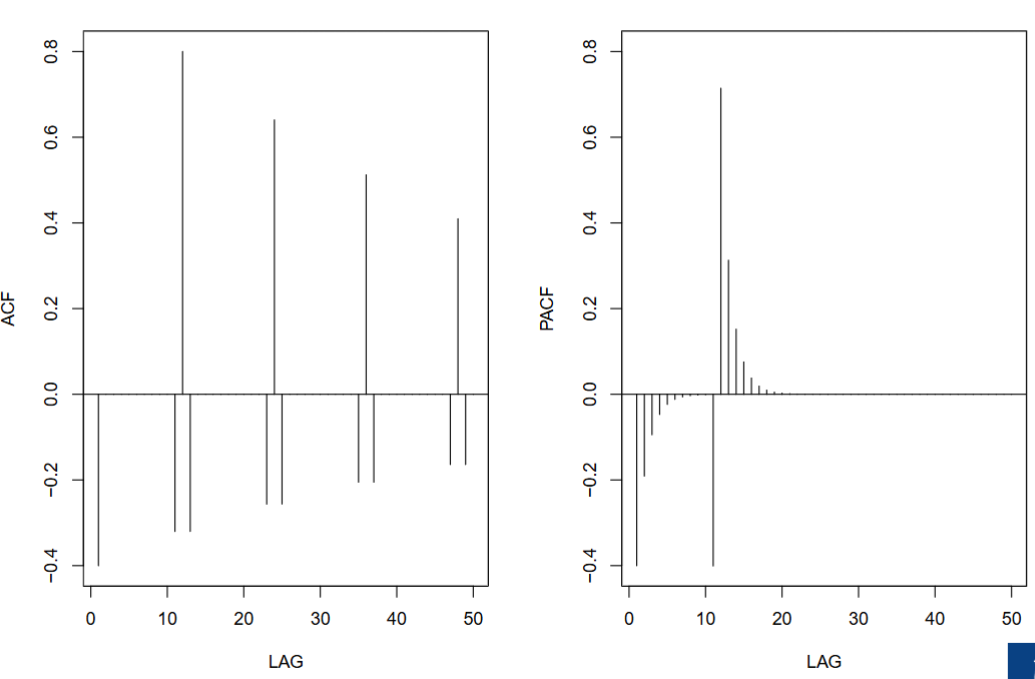
\includegraphics[width=0.8\linewidth]{ARMA multiplicative seasonal model - acf and pacf plot.png}
\end{figure}

\subsection{SARIMA model ARIMA(p, d, q) x (P, D, Q)_s}
\noi \textbf{Seasonal differencing}:
\begin{itemize}
    \item Can be indicated when the ACF decays slowly at multiples of some season $s$, but negligible between the seasons.
    \item Seasonal difference of order $D$ means $\nabla_{s}^{D}x_t = (1 - B^s)^Dx_t$.
    \item Typically, $D = 1$ is sufficient to obtain seasonal stationarity
\end{itemize} \phantom{i}

\noi \textbf{SARIMA Model}: \\
\noi Of the form
$$\Phi_P(B^s)\phi(B)\nabla_{s}^{D}\nabla^{d}x_t = \delta + \Theta_Q(B^s)\theta(B)w_t$$
\noi Note:
\begin{itemize}
    \item Denoted as $ARIMA(p, d, q) \times (P, D, Q)_s$.
    \item Ordinary difference: $\nabla^d = (1-B)^d$ and seasonal difference: $\nabla_{s}^{D} = (1-B^s)^D$
    \item Non-seasonal MA component has polynomial $\theta(B)$ with order $q$. Non seasonal AR component has polynomial $\phi(B)$ with order $p$.
    \item Seasonal MA component has polynomial $\Theta(B)$ with order $Q$. Seasonal AR component has polynomial $\Phi(B)$ with order $P$.
\end{itemize} \phantom{i}

\noi \textbf{Example: a typical SARIMA model} $\boldsymbol{ARIMA(0, 1, 1) \times (0, 1, 1)_{12}}$: \\
\noi We set $\delta = 0$: $\nabla_{12}\nabla x_t = \Theta(B^{12})\theta(B)w_t$. Can also be represented as:
\begin{align*}
    (1-B^{12})(1-B)x_t &= (1 + \Theta B^{12})(1 + \theta B)w_t \\
    (1 - B - B^{12} + B^{13})x_t &= (1 + \theta B + \Theta B^{12} + \Theta \theta B^{13})w_t \\
    x_t &= x_{t-1} + x_{t-12} - x_{t-13} + w_t + \theta w_{t-1} + \Theta w_{t-12} + \Theta\theta w_{t-13}
\end{align*} 

\noi \textbf{Example: Air Passengers dataset} \\
\begin{lstlisting}
x = AirPassengers
plot.ts(x, main = "Air Passengers series, unmodified")
# shows trend and increasing variance so should try log transformation

lx = log(x)
plot.ts(lx, main = "Log of Air Passenger series") # this stabilised the variance

dlx = diff(lx) # try differencing to remove the trend
plot.ts(dlx, main = "Differenced Log of Air Passenger series")
# There is still persistence in spikes with the seasons dlx_t approx. equal dlx_[t-12]

ddlx = diff(dlx, 12) # apply twelvth-order difference on differenced data
plot.ts(ddlx) # improved the seasonality

# Aggregating graphs even more not more analysis though
par(mfrow=c(2,1), mar=c(3,3,2,1), mgp=c(1.6,0.6,0))
monthplot(dlx) # mean on monthly basis vaies a lot
monthplot(ddlx) # mean on a monthly basis is very similar
plot.ts(cbind(x, lx, dlx, ddlx), main = "") # shows all plots together
\end{lstlisting}

\subsection{Multivariate time series - VAR(p) models}
\begin{itemize}
    \item Many data sets involve more than one time series, and we are often interested in the possible dynamics relating all series.
    \item Thus we are interested in modelling and forecasting $k \times 1$ vector-valued time series:
        $$x_t = (x_{t1}, ..., x_{tk})', \: \: t=0, \pm 1, \pm 2,...$$
    \item The \textit{univariate} AR model can be extended to the \textit{Vector} Auto-Regressive (VAR) model.
\end{itemize}

\subsubsection{VAR(1) model}
\noi Of the form
$$x_t = \alpha + \boldsymbol{\phi}x_{t-1} + w_t, $$
\noi Where,
\begin{itemize}
    \item $\boldsymbol{\phi}$ is a $k \times k$ transition matrix, that expresses the dependence of $x_t$ on $x_{t-1}$ (not these are vectors).
    \item The vector white noise process $w_t$ is assumed to be multivariate normal with mean-zero and covariance matrix $\mathbb{E}[w_tw_t'] = \Sigma_w$.
    \item The vector $\alpha = (\alpha_1, \alpha_2, ..., \alpha_k)'$ is similar to a constant in the regression setting. If $\mathbb{E}[x_t] = \mu$, then $\alpha = (\boldsymbol{I} - \boldsymbol{\phi})\mu$, as before.
\end{itemize} \phantom{i}

\noi \textbf{Example: Mortality, Temperature, Pollution}: \\
\begin{itemize}
    \item Define: $x_t = (x_{t1}, x_{t2}, x_{t3})'$, as a vector of dimension $k=3$ for cardiovascular mortality $x_{t1}$, temperature $x_{t2}$, and particulate levels $x_{t3}$.
    \item We might envision dynamic relations with first order relation
        \begin{align*}
            x_{t1} &= \alpha_1 + \beta_1t + \phi_{11}x_{t-1,1} + \phi_{12}x_{t-1,2} + \phi_{13}x_{t-1,3} + w_{t1} \\
            x_{t2} &= \alpha_2 + \beta_2t + \phi_{21}x_{t-1,1} + \phi_{22}x_{t-1,2} + \phi_{23}x_{t-1,3} + w_{t2} \\
            x_{t3} &= \alpha_3 + \beta_3t + \phi_{31}x_{t-1,2} + \phi_{32}x_{t-1,2}  + \phi_{33}x_{t-1,3} + w_{t3} 
        \end{align*}
    \item Also can be written in matrix form as
        $$x_t = \Gamma u_t + \phi x_{t-1} + w_t$$
        \begin{itemize}
            \item Where $\Gamma = [\alpha|\beta]$ is $3 \times 2$ and $u_t = (1,t)'$ is $2 \times 1$
        \end{itemize}
\end{itemize} \phantom{i}

\noi We use R package \texttt{vars} to fit VAR models via last squares.
\begin{lstlisting}
library(vars)
x = cbind(cmort, tempr, part) # make a vector of datasets
summary(VAR(x, p=1, type="both")) # p=1 for Var(1), "both" fits constant + trend

# VAR Estimation Results:
# ========================= 
# Endogenous variables: cmort, tempr, part 
# Deterministic variables: both 
# Sample size: 507 
# Log Likelihood: -5116.02 
# Roots of the characteristic polynomial:
# 0.8931 0.4953 0.1444 <- IN VAR WE WANT THESE |z| < 1. Good!
# Call:
# VAR(y = x, p = 1, type = "both")

# Estimation results for equation cmort: 
# ====================================== 
# cmort = cmort.l1 + tempr.l1 + part.l1 + const + trend 
# 
#           Estimate Std. Error t value Pr(>|t|)    
# cmort.l1  0.464824   0.036729  12.656  < 2e-16 ***
# tempr.l1 -0.360888   0.032188 -11.212  < 2e-16 ***
# part.l1   0.099415   0.019178   5.184 3.16e-07 ***
# const    73.227292   4.834004  15.148  < 2e-16 ***
# trend    -0.014459   0.001978  -7.308 1.07e-12 ***
# ---
# Signif. codes:  0 ‘***’ 0.001 ‘**’ 0.01 ‘*’ 0.05 ‘.’ 0.1 ‘ ’ 1
# 
# 
# Residual standard error: 5.583 on 502 degrees of freedom
# Multiple R-Squared: 0.6908,	Adjusted R-squared: 0.6883 
# F-statistic: 280.3 on 4 and 502 DF,  p-value: < 2.2e-16

# Estimation results for equation tempr: 
# ====================================== 
# tempr = cmort.l1 + tempr.l1 + part.l1 + const + trend
# 
#           Estimate Std. Error t value Pr(>|t|)    
# cmort.l1 -0.244046   0.042105  -5.796 1.20e-08 ***
# tempr.l1  0.486596   0.036899  13.187  < 2e-16 ***
# part.l1  -0.127661   0.021985  -5.807 1.13e-08 ***
# const    67.585598   5.541550  12.196  < 2e-16 ***
# trend    -0.006912   0.002268  -3.048  0.00243 ** 
# ---
# Signif. codes:  0 ‘***’ 0.001 ‘**’ 0.01 ‘*’ 0.05 ‘.’ 0.1 ‘ ’ 1
# 
# 
# Residual standard error: 6.4 on 502 degrees of freedom
# Multiple R-Squared: 0.5007,	Adjusted R-squared: 0.4967 
# F-statistic: 125.9 on 4 and 502 DF,  p-value: < 2.2e-16 

# Estimation results for equation part: 
# ===================================== 
# part = cmort.l1 + tempr.l1 + part.l1 + const + trend 
# 
#           Estimate Std. Error t value Pr(>|t|)    
# cmort.l1 -0.124775   0.079013  -1.579    0.115 <- MORTALITY NOT SIG. TO PREDICT POLLUTION   
# tempr.l1 -0.476526   0.069245  -6.882 1.77e-11 ***
# part.l1   0.581308   0.041257  14.090  < 2e-16 ***
# const    67.463501  10.399163   6.487 2.10e-10 ***
# trend    -0.004650   0.004256  -1.093    0.275    
# ---
# Signif. codes:  0 ‘***’ 0.001 ‘**’ 0.01 ‘*’ 0.05 ‘.’ 0.1 ‘ ’ 1
# 
# 
# Residual standard error: 12.01 on 502 degrees of freedom
# Multiple R-Squared: 0.3732,	Adjusted R-squared: 0.3683 
# F-statistic: 74.74 on 4 and 502 DF,  p-value: < 2.2e-16 

# Covariance matrix of residuals:
#        cmort  tempr   part
# cmort 31.172  5.975  16.65
# tempr  5.975 40.965  42.32
# part  16.654 42.323 144.26
# 
# Correlation matrix of residuals:
#        cmort  tempr   part
# cmort 1.0000 0.1672 0.2484
# tempr 0.1672 1.0000 0.5506
# part  0.2484 0.5506 1.0000
\end{lstlisting}
\noi By inspecting the top triangle of the correlation matrix of residuals the values are pretty large suggesting not white noise (note: this is not a formal way to test this!)

\subsubsection{Var(p) models}
\begin{itemize}
    \item It is easy to extend $Var(1)$ process to higher orders (with correlations going farther than one step into the past), leading to $Var(p)$.
    \item The regressors are $(1, x_{t-1}', x_{t-2}', ..., x_{t-p}')'$.
    \item The regression model is then
        $$x_t = \alpha + \sum_{j=1}^{p}\boldsymbol{\phi}_jx_{t-j} + w_t$$
    \item The R function \texttt{VARselect} suggests the optimal order $p$ according to different criteria:
        \begin{itemize}
            \item AIC,
            \item Hannan-Quinn (similar to BIC),
            \item BIC (called $SC(n)$ in the R function output),
            \item Final Prediction Error (minimises the approximate mean squared one-step-ahead prediction error).
        \end{itemize}
\end{itemize}

\noi \textbf{Example:} $\boldsymbol{VAR(p)}$ \textbf{on Mortality, Temperature, Pollution}: \\
\noi First look for optimal $p$ order value. Note that the \textbf{smaller} the order the better as we always prefer a smaller model than a larger one.
\begin{lstlisting}
library(vars)
VARselect(x, lag.max = 10, type = "both")
# $selection
# AIC(n)  HQ(n)  SC(n) FPE(n) 
#      9      5      2      9 <- 9 IS GOOD BUT WE PREFER SIMPLER 2 MODEL
#
# $criteria
#               1        2        3        4        5
# AIC(n) 11.73780 11.30185 11.26788 11.23030 11.17634
# HQ(n) 11.78758 11.38149 11.37738 11.36967 11.34557
# SC(n) 11.86463 11.50477 11.54689 11.58541 11.60755
# FPE(n) 125216.91717 80972.28678 78268.19568 75383.73647 71426.10041
#               6        7        8        9       10
# AIC(n) 11.15266 11.15247 11.12878 11.11915 11.12019
# HQ(n) 11.35176 11.38144 11.38760 11.40784 11.43874
# SC(n) 11.65996 11.73587 11.78827 11.85473 11.93187
# FPE(n) 69758.25113 69749.89175 68122.40518 67476.96374 67556.45243
\end{lstlisting}
\noi So we will proceed with $p=2$ according to $BIC$.

\begin{lstlisting}
library(vars)
summary(fit <- VAR(x, p = 2, type = "both"))

# VAR Estimation Results:
# ========================= 
# Endogenous variables: cmort, tempr, part 
# Deterministic variables: both 
# Sample size: 506 
# Log Likelihood: -4987.186 
# Roots of the characteristic polynomial:
# 0.8807 0.8807 0.5466 0.4746 0.4746 0.4498 <- STILL < 1 SO GOOD!
# Call:
# VAR(y = x, p = 2, type = "both")

# Estimation results for equation cmort: 
# ====================================== 
# cmort = cmort.l1 + tempr.l1 + part.l1 + cmort.l2 + tempr.l2 + part.l2 + const + trend 
# 
#           Estimate Std. Error t value Pr(>|t|)    
# cmort.l1  0.297059   0.043734   6.792 3.15e-11 ***
# tempr.l1 -0.199510   0.044274  -4.506 8.23e-06 ***
# part.l1   0.042523   0.024034   1.769  0.07745 .  
# cmort.l2  0.276194   0.041938   6.586 1.15e-10 ***
# tempr.l2 -0.079337   0.044679  -1.776  0.07639 .  
# part.l2   0.068082   0.025286   2.692  0.00733 ** 
# const    56.098652   5.916618   9.482  < 2e-16 ***
# trend    -0.011042   0.001992  -5.543 4.84e-08 ***
# ---
# Signif. codes:  0 ‘***’ 0.001 ‘**’ 0.01 ‘*’ 0.05 ‘.’ 0.1 ‘ ’ 1
# 
# 
# Residual standard error: 5.295 on 498 degrees of freedom
# Multiple R-Squared: 0.7227,	Adjusted R-squared: 0.7188 
# F-statistic: 185.4 on 7 and 498 DF,  p-value: < 2.2e-16 

# Estimation results for equation tempr: 
# ====================================== 
# tempr = cmort.l1 + tempr.l1 + part.l1 + cmort.l2 + tempr.l2 + part.l2 + const + trend 
# 
#           Estimate Std. Error t value Pr(>|t|)    
# cmort.l1 -0.108889   0.050667  -2.149  0.03211 *  
# tempr.l1  0.260963   0.051292   5.088 5.14e-07 ***
# part.l1  -0.050542   0.027844  -1.815  0.07010 .  
# cmort.l2 -0.040870   0.048587  -0.841  0.40065    
# tempr.l2  0.355592   0.051762   6.870 1.93e-11 ***
# part.l2  -0.095114   0.029295  -3.247  0.00125 ** 
# const    49.880485   6.854540   7.277 1.34e-12 ***
# trend    -0.004754   0.002308  -2.060  0.03993 *  
# ---
# Signif. codes:  0 ‘***’ 0.001 ‘**’ 0.01 ‘*’ 0.05 ‘.’ 0.1 ‘ ’ 1
# 
# 
# Residual standard error: 6.134 on 498 degrees of freedom
# Multiple R-Squared: 0.5445,	Adjusted R-squared: 0.5381 
# F-statistic: 85.04 on 7 and 498 DF,  p-value: < 2.2e-16 

# Estimation results for equation part: 
# ===================================== 
# part = cmort.l1 + tempr.l1 + part.l1 + cmort.l2 + tempr.l2 + part.l2 + const + trend 
# 
#           Estimate Std. Error t value Pr(>|t|)    
# cmort.l1  0.078934   0.091773   0.860 0.390153    
# tempr.l1 -0.388808   0.092906  -4.185 3.37e-05 ***
# part.l1   0.388814   0.050433   7.709 6.92e-14 ***
# cmort.l2 -0.325112   0.088005  -3.694 0.000245 ***
# tempr.l2  0.052780   0.093756   0.563 0.573724    
# part.l2   0.382193   0.053062   7.203 2.19e-12 ***
# const    59.586169  12.415669   4.799 2.11e-06 ***
# trend    -0.007582   0.004180  -1.814 0.070328 .  
# ---
# Signif. codes:  0 ‘***’ 0.001 ‘**’ 0.01 ‘*’ 0.05 ‘.’ 0.1 ‘ ’ 1
# 
# 
# Residual standard error: 11.11 on 498 degrees of freedom
# Multiple R-Squared: 0.4679,	Adjusted R-squared: 0.4604 
# F-statistic: 62.57 on 7 and 498 DF,  p-value: < 2.2e-16 

# Covariance matrix of residuals:
#        cmort  tempr   part
# cmort 28.034  7.076  16.33
# tempr  7.076 37.627  40.88
# part  16.325 40.880 123.45
# 
# Correlation matrix of residuals:
#        cmort  tempr   part
# cmort 1.0000 0.2179 0.2775
# tempr 0.2179 1.0000 0.5998
# part  0.2775 0.5998 1.0000
\end{lstlisting}
\noi By inspecting the top triangle of the correlation matrix of residuals the values are still quite large suggesting not white noise. The not white noise features of the dataset are further exposed in the following \texttt{acf} plots of the residuals where lots of values outside of the C.I. intervals. \\

\noi The \textbf{Portmanteau test rejects the null hypothesis of white noise, suggesting poor fit}:
\begin{lstlisting}
library(vars)
# using fit of p=2 from above code chunk
serial.test(fit, lags.pt = 12, type = "PT.adjusted")
# 	Portmanteau Test (adjusted)
# 
# data:  Residuals of VAR object fit
# Chi-squared = 162.35, df = 90, p-value = 4.602e-06 <- REJECT H_0 SO NOT WHITE NOISE (BAD)!!

# This observation is further confirmed by visual inspection:
acf(resid(fit), 52) # lots of acf outside of C.I. so not white noise for upper triangle plots

# Predictions are produced with
fit.pr = predict(fit, n.ahead = 24, ci = 0.95) # 24 weeks ahead
fanchart(fit.pr) # plot prediction + error, graphs show pretty bad predictions
\end{lstlisting}


\newpage
%%%%%%%%%%%%%%%%%%%%%%%%%%%%%%%%%%%%%%%%%%%%%%%%%%%%%%%%%%%%%%%%%%%%%%%%%%%%%%
\section{Module 10 - Estimation and Forecasting}
\subsection{Behaviour of the ACF and PACF for ARMA Models}
\begin{table}[ht]
\centering
\begin{tabular}{lcc}
\toprule
Model & ACF & PACF \\
\midrule
AR($p$) & Tails off & Cuts off after lag $p$ \\
MA($q$) & Cuts off after lag $q$ & Tails off \\
ARMA($p, q$) & Tails off & Tails off \\
\bottomrule
\end{tabular}
\end{table}

\begin{itemize}[leftmargin=*]
  \item The PACF for MA models behaves much like the ACF for AR models.
  \item The PACF for AR models behaves much like the ACF for MA models.
  \item Since an invertible ARMA model has an infinite AR representation, its PACF will not cut off.
  \item Since a causal ARMA model has an infinite MA representation, its ACF will not cut off.
  \item Remember that the data might have to be detrended and/or transformed first (e.g., to stabilise the variance, apply a log transform), before such analysis is performed.
\end{itemize}

\subsection{Behaviour of ACF and PACF in presence of seasonality}
\begin{table}[ht]
\centering
\renewcommand{\arraystretch}{1.2}
\begin{tabularx}{\textwidth}{lX X X}
\toprule
 & AR($P$)$_s$ & MA($Q$)$_s$ & ARMA($P, Q$)$_s$ \\
\midrule
ACF*  & Tails off at lags $ks$, $k=1,2,\ldots$ 
      & Cuts off after lag $Qs$ 
      & Tails off at lags $ks$, $k=1,2,\ldots$ \\

PACF* & Cuts off after lag $Ps$ 
      & Tails off at lags $ks$, $k=1,2,\ldots$ 
      & Tails off at lags $ks$, $k=1,2,\ldots$ \\
\bottomrule
\end{tabularx}
\end{table}

\vspace{0.5em}
\noindent
\textit{*The values at nonseasonal lags $h \ne ks$, for $k = 1, 2, \ldots$, are zero.}

\vspace{1em}

\begin{itemize}[leftmargin=*]
  \item This can be seen as a generalisation of the previous table (which is the special case $s=1$).
  \item Fitting seasonal auto regressive and moving average components \textbf{first} generally leads to more satisfactory results.
\end{itemize}

\subsection{Box-Jenkins Methodology}
\begin{enumerate}
    \item Determine the integration order $d$ (of the $ARIMA(p, d, q)$) and work on the corresponding $ARMA(p, q)$ by differencing.
    \item Then choose candidates for $p$ and $q$ from examining ACF and PACF
    \item For fixed $p$ and $q$ (candidates), estimate parameters via:
        \begin{itemize}
            \item Method of moments
            \item Maximum likelihood (much less efficient when $q > 0$)
            \item Least squares and variations
        \end{itemize}
    \item Perform diagnostics, to choose the best $p$ and $q$. Thus may suggest new candidates for $p$ and $q$, in which case we perform a new iteration from step 2.
    \item Use the chosen model for forecasting.
\end{enumerate} \phantom{i}

\noi \textbf{Example of Box-Jenkins steps}: \\

\noi \textbf{Step 1} (choosing $d$): \\
\noi Choosing $d$ involves:
\begin{itemize}
    \item A time series $x_t$ may be modelled by a stationary ARMA model if the sample ACF decays rapidly. If the decay is slow (and the ACF is positive) then this suggests further differencing.
    \item Let $\sigma_d^2$ be the sample variance of the $\nabla^d x_t$. This quantity should first decrease with $d$ until stationarity is achieved, and then start to increase. Hence $d$ could be set to the value which minimises $\sigma_d^2$, $d \geq 0$.
\end{itemize}
\noi Be careful not to over-difference, as this introduces artificial dependence in the data. \\

\noi FYI WITH SEASONALITY IF $d + D \leq 1$ initially fit a constant term then drop if it is not significant. \\

\noi \textbf{Step 2} (choosing $p$ and $q$):
\begin{itemize}
    \item We work on the differenced series, which we assume is $ARMA(p, q)$ and has mean $0$. If the mean is $\neq 0$, subtract its sample mean, and work on the residuals.
    \item Examine ACF and PACF to choose candidates for $p$ and $q$:
        \begin{itemize}
            \item $p$ can be inferred from the number of spikes in the PACF until a geometrical decay to zero is observed.
            \item $q$ can be inferred from the number of spikes in the ACF until a geometrical decay to zero is observed.
        \end{itemize}
    \item alternatively, work iteratively from the simplest models and increase orders $p$ and $q$:
        \begin{itemize}
            \item Higher orders will always reduce the sum of squares (more parameters) - at the extreme model with $n$ parameters will replicate the data.
            \item The approximate order could be chosen by using information critera (e.g. BIC or AIC).
        \end{itemize}
\end{itemize}

\begin{lstlisting}
acf2(rec, 48) # recruitment series for 48 months of lag
\end{lstlisting}
\noi The ACF decays straight away (so $q \approx 0$) and PACF has 2 spikes then decays (so $p \approx 2$). \\

\noi \textbf{Step 3} (estimation of parameters): \\
\begin{itemize}
    \item We now need estimates for $\phi_1,...,\phi_p$ and $\theta_1,...,\theta_q$ for given $p$ and $q$
    \item Use R to fit model with \texttt{fit <- arima(x, order = c(p, 0, q))}, where \texttt{x} is differenced series and where \texttt{p} and \texttt{q} are the values from before.
    \item The default estimation procedure (unless there are missing values) is to use conditional sum-of-squares to find starting values, then maximum likelihood.
    \item This output parameter estimates, their standard errors, as well as $\sigma^2$ and the AIC.
    \item One could alternatively use methods of moments approach (see later), but this is much less efficient than MLE if $q > 0$.
\end{itemize}
\noi Code for MLE values for just AR general case below
\begin{lstlisting}
rec.mle = ar.mle(rec, order = 2)
rec.mle$x.mean
# [1] 62.26153
rec.mle$ar
# [1] 1.3512809 -0.4612736
sqrt(diag(rec.mle$asy.var.coef))
# [1] 0.04099159 0.04099159
rec.mle$var.pred # the PROPORTION NOT EXPLAINED by the model (so not good)
# [1] 89.33597

# The fit is displayed as follows
ts.plot(rec, main = "Results of fit using the R MLE estimators")
lines(rec[1:length(rec)] - rec.mle$resid, col = "blue", lwd = 1)
\end{lstlisting}

\noi \textbf{Best estimators general ARMA case} (gives very similar values to above, but uses different estimation procedure): \\

\begin{lstlisting}
rec.arima0 <- arima(rec, order = c(2, 0, 0)) # to use with tsdiag

rec.arima0$coef[3]
# intercept 
# 61.85847
rec.arima0$coef[1:2]
#       ar1        ar2
# 1.3512196 -0.4612128
sqrt(diag(rec.arima0$var.coef))
#        ar1        ar2  intercept
# 0.04158461 0.04166812 4.00393366
rec.arima0$sigma2
# [1] 89.33436

# The fit is displayed as follows
ts.plot(rec, main = "Residuals of fit using R ARIMA estimators")
lines(rec[1:length(rec)] - rec.arima0$residuals, col = "blue", lwd = 1)
\end{lstlisting} \phantom{i}

\noi \textbf{Step 4} (diagnostics): \\
\noi Guiding principle: if we have a good fit, the residuals should be (uncorrelated) white noise. This can be done in three ways (can be done in R using \texttt{tsdiag(fit)}, but better to use \texttt{sarima(x, p, d, q} from \texttt{astsa}):
\begin{enumerate}
    \item \textbf{Residuals}: If visual inspection of the residuals exhibit any pattern (trend or magnitude) then these are not white noise.
    \item \textbf{ACF and PACF}: These should be within the confidence intervals with approximate frequency ($95\%$)
    \item \textbf{Ljung-Box Portmanteau Test} (most formal): This test considers the dimensions of the models (number of parameters), and tests whether correlations are $0$ at all lags, and displays $p$-values. High $p$-values mean we cannot reject the (null) hypothesis of white noise (which is what we want).
\end{enumerate}

\begin{lstlisting}
tsdiag(rec.arima0)
\end{lstlisting}
\begin{figure}[H]
    \centering
    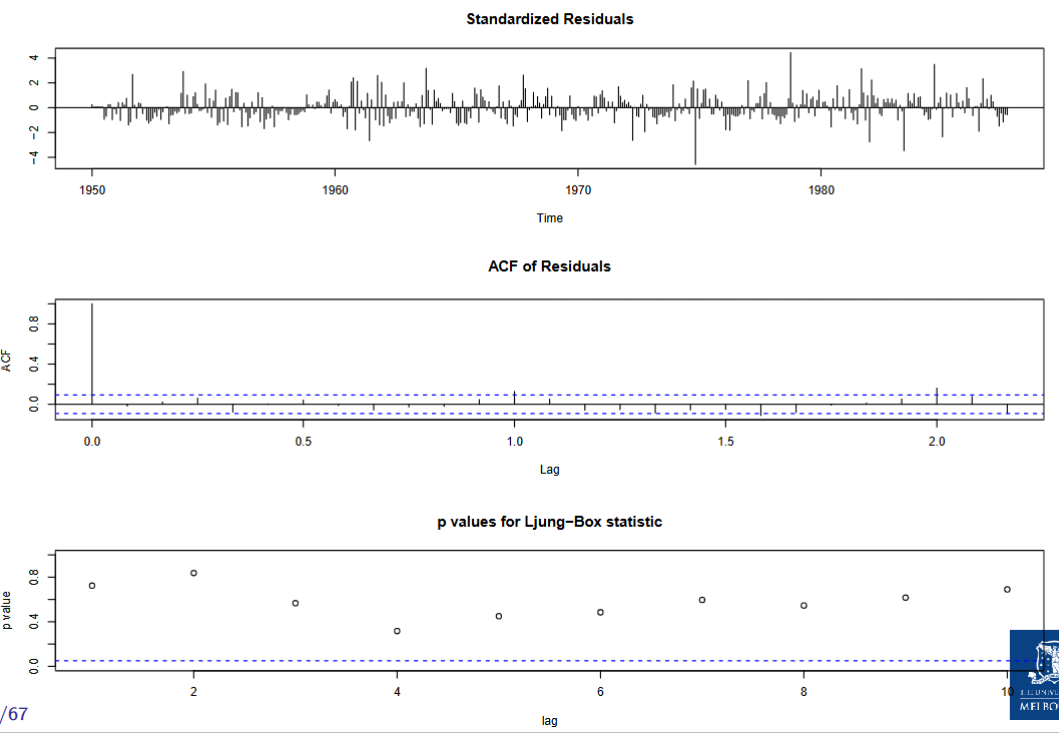
\includegraphics[width=0.8\linewidth]{tsdiag results for Box-Jenkins Example.png}
\end{figure}
\noi Notes: Too many spikes ($3/26$) outside of confidence interval, so bad.

\begin{lstlisting}
RecSARIMAdig <- sarima(rec, 2, 0, 0)
\end{lstlisting}
\begin{figure}[H]
    \centering
    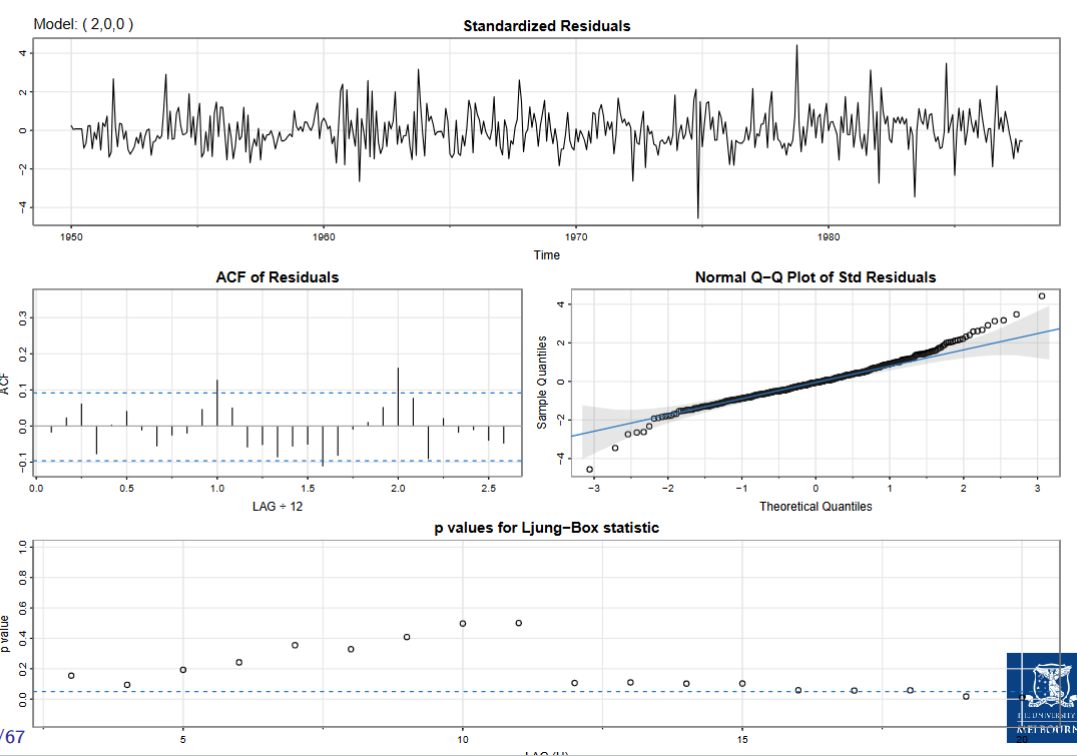
\includegraphics[width=0.8\linewidth]{sarima results for Box-Jenkins Example.png}
\end{figure}
\noi Notes: In Q-Q plot lots of dots outside of C.I. (bad), too many ACF spikes outside of C.I. (bad), and sharp drop in $p$-values for Ljung-Box statistic (bad, sharp drop at $12$ suggests seasonality).

\begin{lstlisting}
RecSARIMAdiag$fit

# Call:
# arima(x = xdata, order = c(p, d, q), seasonal = list(order = c(P, D, Q),
#     xreg = xmean, include.mean = FALSE, transform.pars = trans, fixed =
#     optim.control = list(trace = trc, REPORT = 1, reltol = tol))
#
# Coefficients:
#         ar1     ar2   xmean
#      1.3512 -0.4612 61.8585
# s.e. 0.0416 0.0417 4.0039
#
# sigma^2 estimated as 89.33: log likelihood = -1661.51, aic = 3331.02 <- AIC FOR WHOLE MODEL
RecSARIMAdiag$ICs
#      AIC     AICc      BIC
# 7.353244 7.353362 7.389587 <- GIVES AIC PER DATA POINT (to get above do 7.35 x # data points)
\end{lstlisting}

\subsubsection{Example: Air Passengers}
\noi From before we already found that taking $12^{th}$ order difference (seasonal), on the differenced logged data makes the residuals look reasonably stationary.
\begin{lstlisting}
x = AirPassengers
lx = log(x)
dlx = diff(lx)
ddlx = diff(dlx, 12)

acf2(ddlx, 50) # ACF and PACF for data
\end{lstlisting}
\begin{figure}[H]
    \centering
    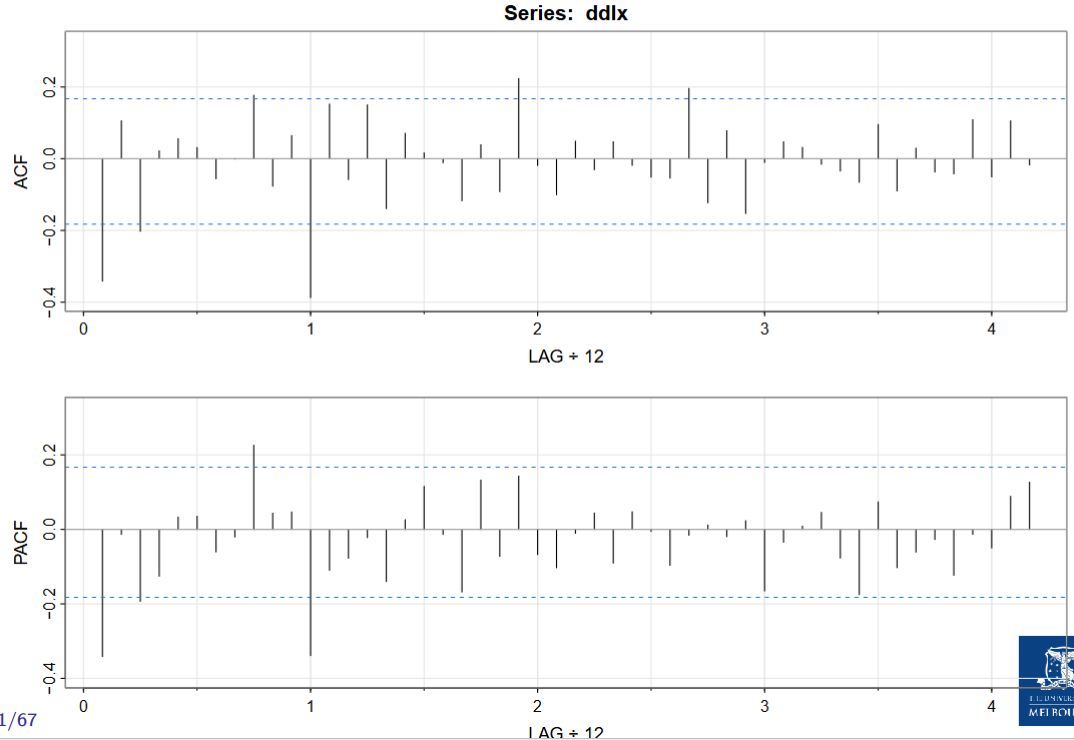
\includegraphics[width=0.8\linewidth]{air passengers data set acf and pacf plots.png}
\end{figure}

\noi Seasonal component:
\begin{itemize}
    \item At the seasons, the ACF appears to be cutting off at lag $1s$ $(s=12)$
    \item PACF appears to be tailing off at lags $1s, 2s, 3s, 4s,...$
    \item $\implies SMA(1)$, $P=0$, $Q=1$, in the seasons $s=12$ 
\end{itemize}

\noi Non-seasonal component:
\begin{itemize}
    \item We inspect the ACF and PACF at lower lags
    \item Both appear to be tailing off, which suggests ARMA within the seasons, say with $p = q = 1$
    \item $\implies ARMA(1,1)$
\end{itemize}

\noi Thus, we will first try an $ARIMA(1,1,1) \times (0,1,1)_{12}$ on the logged data
\begin{lstlisting}
AirPassFit1 = sarima(lx, 1, 1, 1, 0, 1, 1, 12)
# sarima(data, p, d, q, P, D, Q, s)
# could use ddlx: sarima(ddlx, 1, 0, 1, 0, 0, 1, 12)
AirPassFit1$fit
## Call:
## arima(x = xdata, order = c(p, d, q), seasonal = list(order = c(P, D, Q),
## include.mean = !no.constant, transform.pars = trans, fixed = fixed,
## REPORT = 1, reltol = tol))
##
## Coefficients:
##         ar1     ma1    sma1
##      0.1960 -0.5784 -0.5643
## s.e. 0.2475  0.2132  0.0747 # <- AR parameter is not significant too high, so drop it
##
## sigma^2 estimated as 0.001341: log likelihood = 244.95, aic = -481.9

# We can try other models to test
AirPassFit2 <- sarima(lx, 0, 1, 1, 0, 1, 1, 12) # ARIMA(0,1,1)x(0,1,1)_12
AirPassFit3 <- sarima(lx, 1, 1, 0, 0, 1, 1, 12) # ARIMA(1,1,0)x(0,1,1)_12

AirPassFit2$fit
## Coefficients:
##         ma1    sma1
##     -0.4018 -0.5569
## s.e. 0.0896 0.0731
##
## sigma^2 estimated as 0.001348: log likelihood = 244.7, aic = -483.4

AirPassFit3$fit
## Coefficients:
##         ar1    sma1
##     -0.3395 -0.5619
## s.e. 0.0822 0.0748
##
## sigma^2 estimated as 0.001367: log likelihood = 243.74, aic = -481.49

AirPassFit2$ICs
##       AIC      AICc       BIC
## -3.690069 -3.689354 -3.624225

AirPassFit3$ICs
##       AIC      AICc       BIC
## -3.675493 -3.674777 -3.609649

# INFORMATION CRITERIA FOR Fit2 is LOWER SO BETTER, SO TRY THAT MODEL!
AirPassFit2 <- sarima(lx, 0, 1, 1, 0, 1, 1, 12) # ARIMA(0,1,1)x(0,1,1)_12
\end{lstlisting}
\begin{figure}[H]
    \centering
    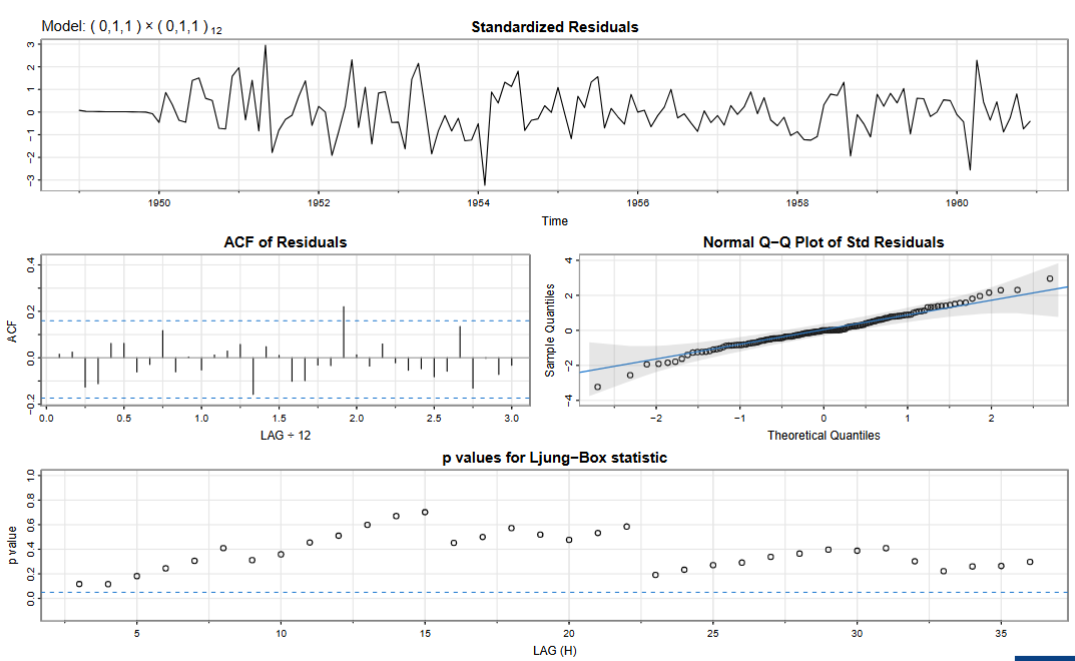
\includegraphics[width=0.8\linewidth]{Air Passengers Diagnostic Plots Updated Model.png}
\end{figure}
\noi Except for 1-2 outliers, the model fits well.

\subsubsection{Example: GNP data}
\begin{lstlisting}
plot(gnp, main = "Quartely U.S. GNP")
# data seems to have exponential growth, so a log transformation is appropriate

acf2(gnp, 50, main = "Sample ACF and PACF of the GNP data")
# slow decay of ACF => differencing may be appropriate

# Making the modifications:
gnp.log.diff = diff(log(gnp)) # growth rate plot(gnpgr)
ts.plot(gnp.log.diff, main="")
abline(mean(gnp.log.diff), 0, col = "blue", lwd = 2) # plots mean

acf2(gnp.log.diff, 24)
\end{lstlisting}
\begin{figure}[H]
    \centering
    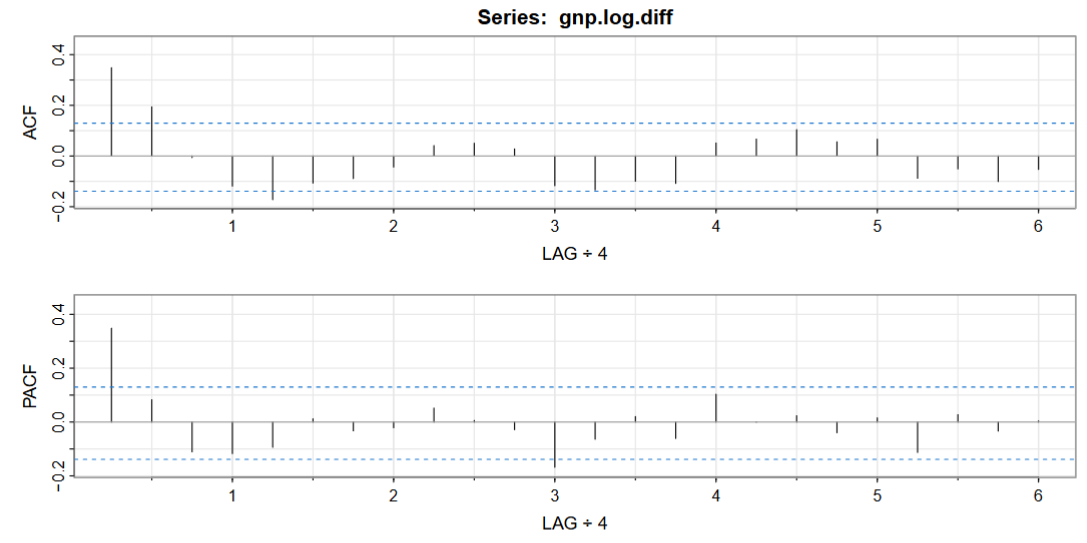
\includegraphics[width=0.8\linewidth]{GNP ACF and PACF plot.png}
\end{figure}
\noi Note: we can see the ACF cuts off after second lag (potential $MA(2)$). The PACF seems to cut off after first lag (potential $AR(1)$) \\

\noi \textbf{GNP data: MA(2) fit}
\begin{lstlisting}
GNP.MA2 <- sarima(gnp.log.diff, 0, 0, 2) # MA(2)
GNP.MA2$fit
## Call:
## arima(x = xdata, order = c(p, d, q), seasonal = list(order = c(P, D, Q),
##      xreg = xmean, include.mean = FALSE, transform.pars = trans, fixed =
##      optim.control = list(trace = trc, REPORT = 1, reltol = tol))
##
## Coefficients:
##         ma1    ma2  xmean
##      0.3028 0.2035 0.0083
## s.e. 0.0654 0.0644 0.0010
##
## sigma^2 estimated as 8.919e-05: log likelihood = 719.96, aic = -1431.9
GNP.MA2$ICs
##       AIC      AICc       BIC
## -6.450133 -6.449637 -6.388823
\end{lstlisting}
\begin{figure}[H]
    \centering
    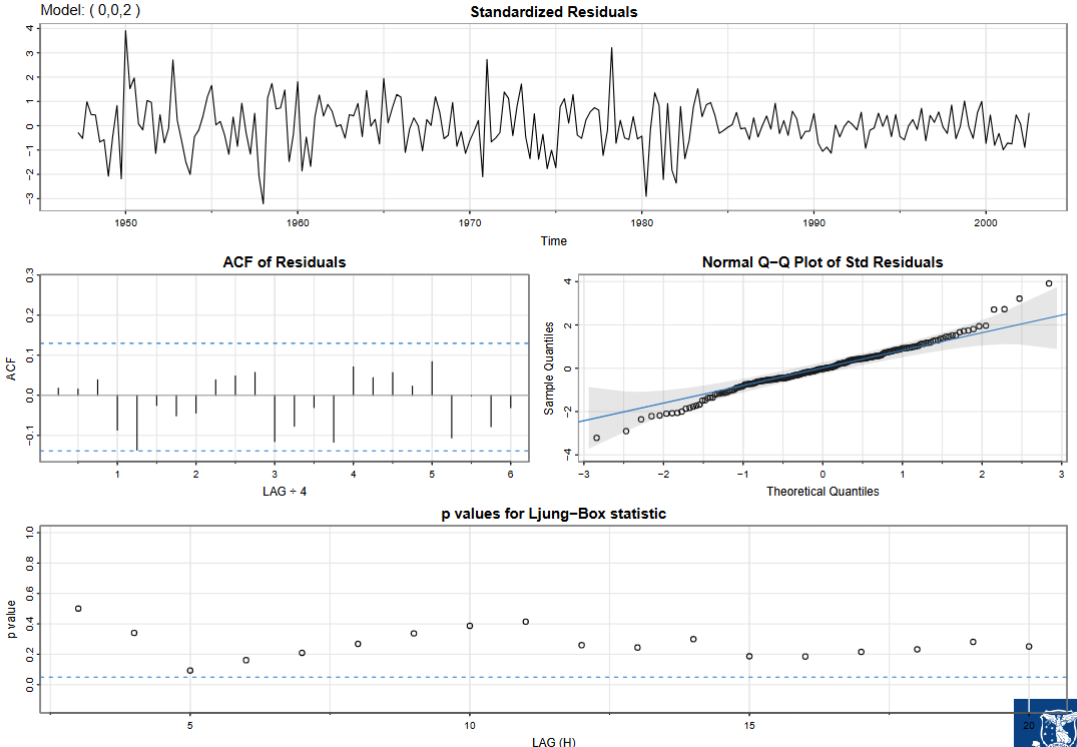
\includegraphics[width=0.7\linewidth]{GNP data MA(2) fit.png}
\end{figure}

\noi \textbf{GNP data: AR(1) fit}
\begin{lstlisting}
GNP.AR1 <- sarima(gnp.log.diff, 1, 0, 0) # AR(1)
GNP.AR1$fit

## Call:
## arima(x = xdata, order = c(p, d, q), seasonal = list(order = c(P, D, Q),
##      xreg = xmean, include.mean = FALSE, transform.pars = trans, fixed =
##      optim.control = list(trace = trc, REPORT = 1, reltol = tol))
##
## Coefficients:
##         ar1  xmean
##      0.3467 0.0083
## s.e. 0.0627 0.0010
##
## sigma^2 estimated as 9.03e-05: log likelihood = 718.61, aic = -1431.22
GNP.AR1$ICs
##       AIC      AICc       BIC
## -6.446940 -6.446693 -6.400958
\end{lstlisting}
\begin{figure}[H]
    \centering
    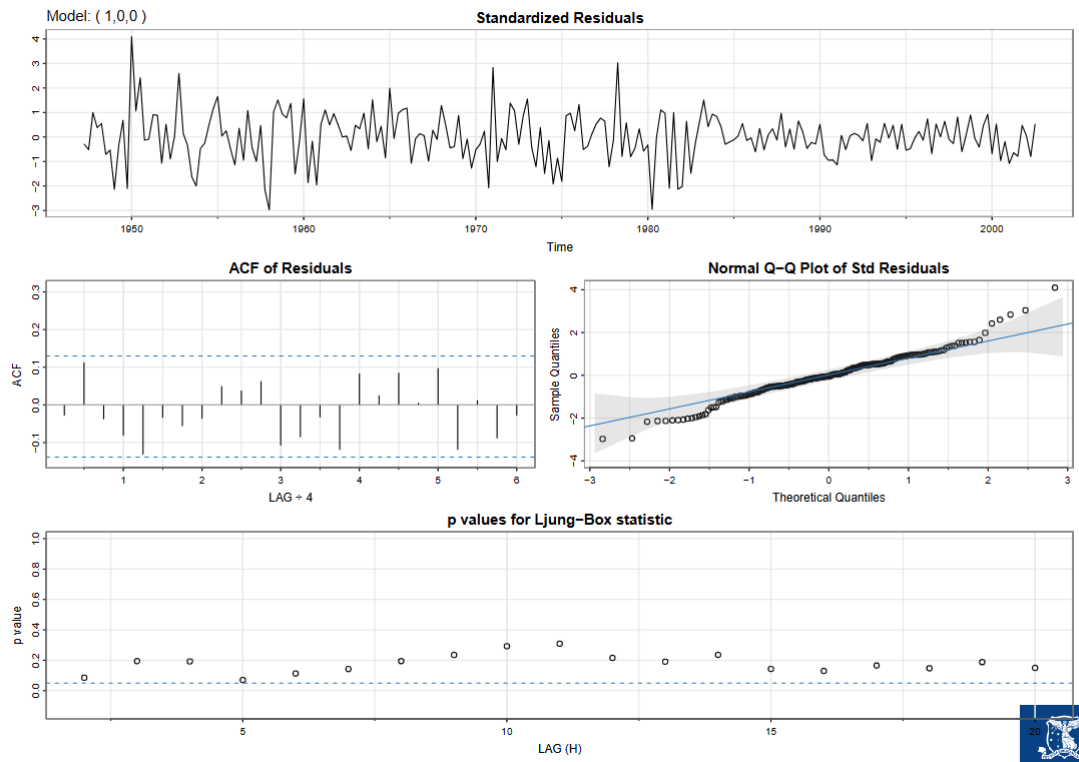
\includegraphics[width=0.7\linewidth]{GNP data AR(1) fit.png}
\end{figure}

\noi \textbf{GNP data: ARMA(1,2) fit}
\begin{lstlisting}
GNP.ARMA <- sarima(gnp.log.diff, 1, 0, 2) # ARMA(1,2)
GNP.ARMA$fit
## Call:
## arima(x = xdata, order = c(p, d, q), seasonal = list(order = c(P, D, Q),
##      xreg = xmean, include.mean = FALSE, transform.pars = trans, fixed =
##      optim.control = list(trace = trc, REPORT = 1, reltol = tol))
##
## Coefficients:
##         ar1    ma1    ma2  xmean
##      0.2407 0.0761 0.1623 0.0083
## s.e. 0.2066 0.2026 0.0851 0.0010 <- SE VERY HIGH for AR1, MA1!!!!
##
## sigma^2 estimated as 8.877e-05: log likelihood = 720.47, aic = -1430.9
GNP.ARMA$ICs
##       AIC      AICc       BIC
## -6.445712 -6.444882 -6.369075
\end{lstlisting}
\begin{figure}[H]
    \centering
    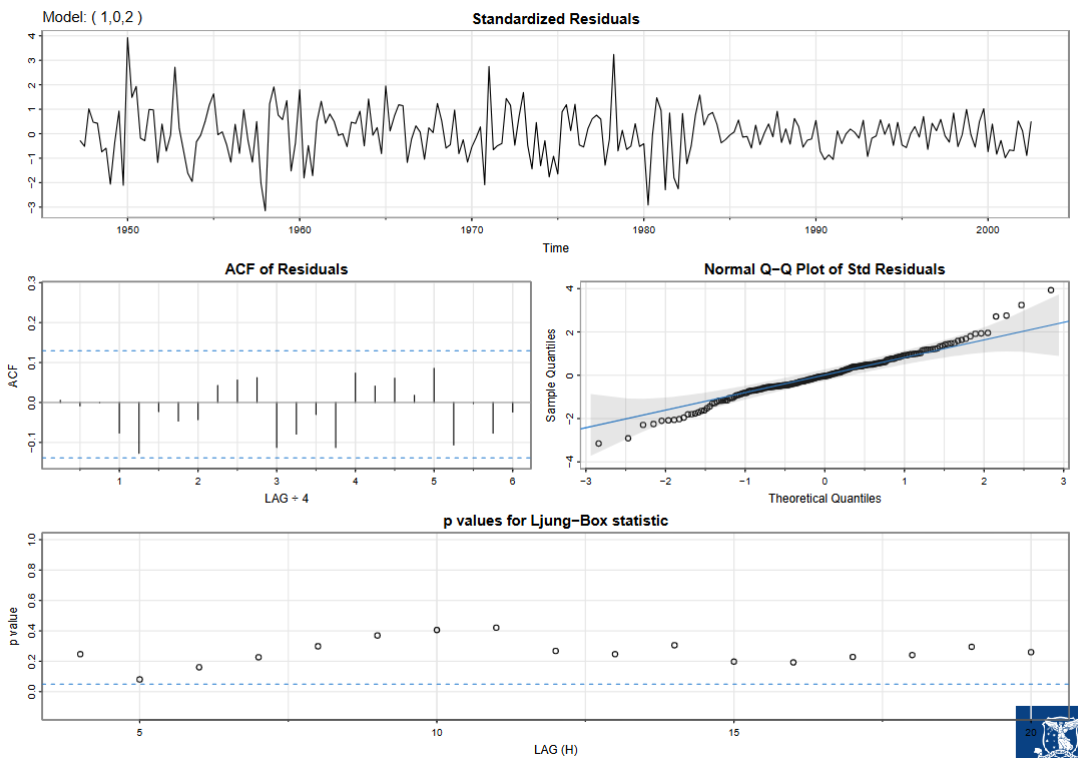
\includegraphics[width=0.7\linewidth]{GNP data ARMA(1,2) fit.png}
\end{figure}
\noi But the graphs look pretty good! \\

\noi \textbf{GNP data: Comparison} \\
\noi Note the fitted models are
\begin{itemize}
    \item $MA(2): \hat{x}_t = 0.008_{(0.001)} + 0.303_{(0.065)}\hat{w}_{t-1} + 0.204_{(0.064)}\hat{w}_{t-2} + \hat{w}_t$, where $\hat{\sigma}_w = 0.0094$.
    \item $AR(1): \hat{x}_t = 0.008_{(0.001)}(1-0.347) + 0.347_{(0.0063)}\hat{x}_{t-1} + \hat{w}_t$, where $\hat{\sigma}_w = 0.0095$.
    \item Both models are nearly the same. This is because the AR model can be rewritten (ignoring the constant) as: $x_t \approx 0.35w_{t-1} + 0.12w_{t-2} + w_t$, where the coefficients are obtained by
        \begin{lstlisting}
            formatC(ARMAtoMA(ar=0.35, ma=0, 6), digits=3)
            ## [1] "0.35" "0.122" "0.0429" "0.015" "0.00525" "0.00184"
        \end{lstlisting}
\end{itemize} \phantom{i}

\noi \textbf{GNP data: Model Selection} \\
\begin{itemize}
    \item Information criteria (the lower the better):
        \begin{itemize}
            \item AR(1): \texttt{\$AIC: -6.446940 \$AICc: -6.446693 \$BIC: -6.400958}
            \item MA(2): \texttt{\$AIC: -6.450133 \$AICc: -6.449637 \$BIC: -6.388823}
            \item ARMA(1,2): \texttt{\$AIC: -6.445712 \$AICc: -6.444882 \$BIC: -6.369075}
        \end{itemize}
    \item The AIC and AICc both prefer the $MA(2)$ fit to $AR(1)$
    \item The BIC prefers the simpler $AR(1)$ model to $MA(2)$
    \item It is often the case that the BIC will select a model of smaller order than the AIC or AICc. In either case, it is not unreasonable to retain the $AR(1)$ because pure AR models are easier to work with.
    \item Combining the two to $ARMA(1,2)$ leads to poorer scores.
\end{itemize}

\subsection{Forecasting - Basics}
\subsubsection{Best Linear Predictors and Prediction for Stationary Processes}
\noi Here we restrict our attention to predictors that are linear functions of the data, that is predictors of the form:
$$x_{n+m}^n = \alpha_0 + \sum_{k=1}^{n}\alpha_kx_k,$$
\noi where $\alpha_0, \alpha_1, ..., \alpha_n$ are real numbers and are the best linear predictors. Note:
\begin{itemize}
    \item The $\alpha$'s depend on $m$ too, but that is not reflected in the notation.
    \item Such estimators depend only on the second-order moments of the process, which are easy to estimate from the data.
\end{itemize} \phantom{i}

\subsubsection*{BLP for Stationary Processes}
\noi Given data $x_1, ..., x_n$, the best linear predictor
$$x_{n+m}^n = \alpha_0 + \sum_{k=1}^{n}{\alpha_k x_k}$$
\noi of $x_{n+m}$ for $m \geq 1$ is found by solving
$$\mathbb{E}[(x_{n+m} - x_{n+m}^n)x_k] = 0, \: \: k=0,1,...,n$$
\noi where $x_0 = 1$, for $\alpha_0, \alpha_1, ..., \alpha_n$
\begin{itemize}
    \item The $n + 1$ equations specified above are called the \textbf{prediction equations}, and they are used to solve for the coefficients $\{\alpha_0, \alpha_1,..., \alpha_n\}$
    \item This result stems from minimising least squares.
\end{itemize} \phantom{i}

If $\mathbb{E}[x_t] = \mu$, the first equation ($k=0$) implies
$$\mathbb{E}[x_{n+m}^n] = \mathbb{E}[x_{n+m}] = \mu$$
\noi Thus, taking expectation of the BLP leads to
$$\mu = \alpha_0 + \sum_{k=1}^{n}{\alpha_k \mu} \: \text{ or } \: \alpha_0 = \mu\Big( 1 - \sum_{k=1}^{n}\alpha_k \Big)$$
\noi Hence, the form of the BLP is
$$x_{n+m}^n = \mu + \sum_{k=1}^{n}\alpha_k(x_k - \mu_k)$$
\noi Henceforth, we will assume that $\mu = 0 \Leftrightarrow \alpha_0 = 0$, wlog, as long as parameters are assumed known.

\subsubsection{One-step-ahead prediction}
\begin{itemize}
    \item Given $\{ x_1,x_2,...,x_n \}$ we wish to forecast the time series $x_{n+1}$ value at the next point in time $n+1$.
    \item The BLP of $x_{n+1}$ is of the form
        $$x_{n+1}^n = \phi_{n1}x_n + \phi_{n2}x_{n-1} + ... + \phi_{nn}x_1$$,
    \item In this case, $\alpha_k$ is $\phi_{n,n+1-k}$ for $k=1,...,n$.
    \item Using BLP result above, the coeffients of $\phi_{ni}$'s satisfy
        $$\sum_{j=1}^{n}{\phi_{nj}\gamma(k-j)} = \gamma(k) \text{ for } k = 1,...,n$$
        \begin{itemize}
            \item Or can be written in matrix form $\Gamma_n\phi_n = \gamma_n$
            \item Where $\Gamma_n = \{\gamma(k-j)\}_{j,k=1}^{n}$, $\phi_n = (\phi_{n1},...,\phi_{nn})'$. Also $\gamma_n = (\gamma(1),...,\gamma(n))'$
            \item The matrix $\Gamma_n$ is non-negative definite (in fact positive definite for ARMA models). We have then
                $$\phi_n = \Gamma_n^{-1}\gamma_n$$
        \end{itemize}
    \item The one-step-ahead forecast is then
        $$x_{n+1}^n = \phi_{n}'x, \text{ where } x=(x_n,x_{n-1},...,x_1)'$$
    \item The mean square one-step-ahead prediction error is
        $$P_{n+1}^n = \mathbb{E}[(x_{n+1} - x_{n+1}^{n})^2] = \gamma(0) - \gamma_n'\Gamma_n^{-1}\gamma_n$$
\end{itemize}

\subsection{Forecasting}
\noi We assume that $x_t$ is a causal and invertible $ARMA(p, q)$ process
$$\phi(B)x_t = \theta(B)w_t, \text{ where } w_t \sim \text{iid N}(0, \sigma_w^2)$$
\noi Note: if there is non-zero mean $\mathbb{E}[x_t] = \mu_x$, simple replace $x_t$ with $x_t - \mu_x$ in the model. \\

\noi \textbf{Two types of forecasts}: \\
\begin{enumerate}
    \item The minimum mean square error predictor of $x_{n+m}$, defined as
        $$x_{n+m}^n = \mathbb{E}[x_{n+m}|x_n,x_{n-1},...,x_1]$$
    \item The predictor of $x_{n+m}$ based on the \textit{infinite} past, defines as
        $$\tilde{x}_{n+m} = \mathbb{E}[x_{n+m}|x_n,x_{n-1},...,x_1,x_0,x_{-1},...]$$
\end{enumerate} \phantom{i}

\noi Note:
\begin{itemize}
    \item For ARMA models, $\tilde{x}_{n+m}$ is easier to calculate.
    \item In general, $x_{n+m}^n$ and $\tilde{x}_{n+m}$ are not the same.
    \item For large samples, $\tilde{x}_{n+m}$ provides a good approximation to $x_{n+m}^{n}$.
\end{itemize}

\subsubsection{Forecasts for more than one step}
\noi Write $x_{n+m}$ in its invertible form:
$$w_{n+m} = \sum_{j=0}^{\infty}{\pi_jx_{n+m-j}}, \quad \pi_0 = 1$$
\noi Taking conditional expectations we have
$$0 = \tilde{x}_{n+m} + \sum_{j=1}^{\infty}{\pi_j\tilde{x}_{n+m-j}} \quad \text{since } \pi_0 =1$$
\noi Because $\mathbb{E}[x_t|x_n,x_{n-1},...,x_0,x_{-1},...] = x_t$ for $t \leq n$ this can be rewritten as
$$\tilde{x}_{n+m} = -\sum_{j=1}^{m-1}{\pi_j\tilde{x}_{n+m-j}} - \sum_{j=m}^{\infty}\pi_jx_{n+m-j}$$
\noi{Prediction is then accomplished recursively using this formula, start with the one-step-ahead ($m=1$), and then continuing for $m=2,3,...$}. \\

\noi \textbf{Finding mean-square prediction error}: \\

\noi Write $x_{n+m}$ in its causal form:
$$x_{n+m} = \sum_{j=0}^{\infty}{\psi_j w_{n+m-j}}, \quad \psi_0 = 1$$
\noi Taking conditional expectations we have
$$\tilde{x}_{n+m} = \sum_{j=0}^{\infty}\psi_j\tilde{w}_{n+m-j} = \sum_{j = m}^{\infty}{\psi_jw_{n+m-j}}$$
\noi Because
$$\tilde{w}_t = \mathbb{E}[w_t|x_n,x_{n-1},...,x_0,x_{-1},...] = \begin{cases}
    0 & t >n, \\
    w_t & t \leq n.
\end{cases}$$

\noi Mean-square prediction error can now be calculated since we now know that
$$\tilde{x}_{n+m} = \sum_{j=m}^{\infty}\psi_jw_{n+m-j} \implies x_{n+m} - \tilde{x}_{n+m} = \sum_{j=0}^{m-1}\psi_jw_{n+m-j}$$
\noi and hence
$$P_{n+m}^{n} = \mathbb{E}[(x_{n+m} - \tilde{x}_{n+m})^2] = \sigma_w^2\sum_{j=0}^{m-1}\psi_j^2$$
\noi Note that for a fixed sample size, $n$, the prediction errors are correlated. That is, for lag $k \geq 1$,
$$\mathbb{E}[(x_{n+m} - \tilde{x}_{n+m})(x_{n+m+k} - \tilde{x}_{n+m+k})] = \sigma_w^{s}\sum_{j=0}^{m-1}{\psi_j\psi_{j+k}}$$

\subsubsection{Predictions in practice}
\begin{itemize}
    \item When $n$ is small the system of "prediction equations" (where $x_0 = 1$)
        $$\mathbb{E}[(x_{n+m} - x_{n+m}^m)x_k] = 0, \quad k=0,1,...,n$$
    \item However, when $n$ is large one will want to use, but in practice we do not observe $x_0, x_{-1},x_{-2},...$ and only $x_1,x_2,..,x_n$ are available. We then need to truncate the infinite sum on the RHS
        $$\tilde{x}_{n+m} = -\sum_{j=1}^{m-1}\pi_j\tilde{x}_{n+m-j} - \sum_{j=m}^{\infty}\pi_jx_{n+m-j}$$
    \item The \textbf{truncated predictor} is then written as (which is applied recursively)
        $$\tilde{x}_{n+m}^n = -\sum_{j=1}^{m-1}\pi_j\tilde{x}_{n+m-j}^{n} - \sum_{j=m}^{n+m-1}\pi_jx_{n+m-j}$$
    \item The mean squared error, in this case, is approximated using $P_{n+m}^n$ as before.
\end{itemize}

\subsubsection{Truncated prediction for ARMA}
\noi For $ARMA(p, q)$ models, the truncated predictors for $m=1,2,...$ are
$$\tilde{x}_{n+m}^n = \phi_1\tilde{x}_{n+m}^n + ... + \phi_p\tilde{x}_{n+m-p}^n + \theta_1\tilde{w}_{n+m-1}^{n} + ... + \theta_q \tilde{w}_{n+m-q}^{n}$$,
\noi where $\tilde{x}_t^n = x_t$ for $1 \leq t \leq n$ and $\tilde{x}_t^n = 0$ for $t \leq 0$. The truncated prediction errors are given by
$$\tilde{w}_t^n = \begin{cases}
    0 & t \leq 0 \text{ or } t >n \\
    \phi(B)\tilde{x}_n^n - \theta_1\tilde{w}_{t-1}^n - ... 0 \theta_q\tilde{w}_{t-q}^{n} & 1 \leq t \leq n
\end{cases}$$
\noi Note:
\begin{itemize}
    \item For $AR(p)$ models with $n > p$ (so there is no need for approximations), 
        $$\tilde{x}_{n+m}^n = \tilde{x}_{n+m} = x_{n+m}^n$$
    \item The above approximation is required for $MA(q)$ and $ARMA(p,q)$ where $q>0$.
\end{itemize}

\subsubsection{Long-range forecasts}
\begin{itemize}
    \item Consider forecasting an ARMA process with mean $\mu_x$
    \item Replacing $x_{n+m}$ with $x_{n+m} - \mu_x$ in the causal representation above, and taking expectation in an analogous way implies that the $m$-step-ahead forecast can be written as
        $$\tilde{x}_{n+m} = \mu_x + \sum_{j=m}^{\infty}\psi_jw_{n+m-j}$$
    \item Because the $\psi$ dampen to zero exponentially fast,
        $$\tilde{x}_{n+m} \rightarrow \mu_x \text{ exponentially fast as } m \rightarrow \infty$$
    \item Moreover, the mean squared prediction error
        $$P_{n+m}^n \rightarrow \sigma_w^2\sum_{j=0}^{\infty}\psi_j^2 = \gamma_x(0) = \sigma_x^2 \text{ exponentially fast as } m \rightarrow \infty$$
    \item ARMA forecasts quickly settle to the mean with a constant prediction error as forecast horizon, m, grows.
\end{itemize} \phantom{i}

\noi \textbf{Forecasting example on recruitment data}
\begin{lstlisting}
rec.arima0 <- arima(rec, order = c(2, 0, 0))
fore2 <- predict(rec.arima0, n.ahead=36)
cbind(fore2$pred, fore2$se)
##         fore2$pred fore2$se
## Oct 1987 20.36547 9.451686
## Nov 1987 26.08036 15.888378
## Dec 1987 32.65148 20.464325
## Jan 1988 38.89474 23.492457
## Feb 1988 44.30006 25.393693
## Mar 1988 48.72437 26.537088
## Apr 1988 52.20958 27.199368
## May 1988 54.87831 27.570234
## Jun 1988 56.87693 27.771616
## Jul 1988 58.34666 27.877923
## Aug 1988 59.41079 27.932597
## Sep 1988 60.17081 27.960042
## Oct 1988 60.70697 27.973508
## Nov 1988 61.08091 27.979974
## Dec 1988 61.33890 27.983014

ts.plot(rec, fore2$pred, col=1:2, xlim=c(1980, 1990.5), ylab="Recruitment")
U = fore2$pred + fore2$se
L = fore2$pred - fore2$se
xx = c(time(U), rev(time(U)))
yy = c(L, rev(U))
polygon(xx, yy, border = 8, col = gray(0.6, alpha=0.2)) # shows CI
lines(fore2$pred, type="p", col=2) # makes red points for forecasts, converges to mean as expected
\end{lstlisting}

\noi \textbf{Forecasting example on Air Passenger data}
\begin{lstlisting}
sarima.for(lx, 12, 0, 1, 1, 0, 1, 1, 12) # the second param gives # forecasts (=12)
\end{lstlisting}

\newpage
%%%%%%%%%%%%%%%%%%%%%%%%%%%%%%%%%%%%%%%%%%%%%%%%%%%%%%%%%%%%%%%%%%%%%%%%%%%%%%
\section{Appendix A - Midsemester Revision Sheet}
$$\text{refer to next page}$$
\includepdf[pages=-]{Midsem Revision Sheet.pdf}
%%%%%%%%%%%%%%%%%%%%%%%%%%%%%%%%%%%%%%%%%%%%%%%%%%%%%%%%%%%%%%%%%%%%%%%%%%%%%%
\section{Appendix B – Detailed Proofs and Derivations}
\subsection{Proof of Sklar’s Theorem (Sketch)}
\noindent Let \((X,Y)\) have continuous marginals \(F_X,F_Y\). Define \(U=F_X(X)\), \(V=F_Y(Y)\). Then \(U,V\sim \text{Uniform}(0,1)\). Define copula:
\[
C(u,v) = \Pr(U \le u,\,V \le v) 
= \Pr\bigl(F_X(X)\le u,\,F_Y(Y)\le v\bigr).
\]
Since \(\{x: F_X(x)\le u\} = \{x: x \le F_X^{-1}(u)\}\),
\[
C(u,v) = \Pr\bigl(X \le F_X^{-1}(u),\,Y \le F_Y^{-1}(v)\bigr) 
= F_{X,Y}(F_X^{-1}(u),\,F_Y^{-1}(v)).
\]
\noindent Conversely, if \(C\) is a copula and \(F_X,F_Y\) are marginals, define:
\[
F_{X,Y}(x,y) = C\bigl(F_X(x),\,F_Y(y)\bigr).
\]
One verifies that:
\[
F_{X,Y}(x,\infty) = C\bigl(F_X(x),1\bigr) = F_X(x), 
\quad
F_{X,Y}(\infty,y) = C\bigl(1,F_Y(y)\bigr) = F_Y(y),
\]
using uniform marginals property of \(C\). Hence the joint CDF has marginals \(F_X, F_Y\).

\subsection{Derivation of Panjer Recursion (Detailed)}
\noindent (See the detailed steps in Module 4, but here we verify coefficient manipulation.)

\subsection{Derivation of Special Cases of Archimedean Copulas}
\subsubsection{Clayton Copula}

\begin{itemize}
  \item \textbf{Direct limit of \(C_\theta(u,v)\):}
    \[
      C_\theta(u,v)
      =\bigl(u^{-\theta}+v^{-\theta}-1\bigr)^{-1/\theta}
      =\exp\!\Bigl[-\tfrac1\theta\ln\bigl(u^{-\theta}+v^{-\theta}-1\bigr)\Bigr].
    \]
    As \(\theta\to0\), use \(u^{-\theta}=e^{-\theta\ln u}=1-\theta\ln u+o(\theta)\) and similarly for \(v\):
    \[
      u^{-\theta}+v^{-\theta}-1
      =1-\theta(\ln u+\ln v)+o(\theta),
      \quad
      -\tfrac1\theta\ln(\cdots)\to\ln u+\ln v,
    \]
    so
    \[
      \lim_{\theta\to0}C_\theta(u,v)
      =\exp(\ln u+\ln v)=uv.
    \]
    As \(\theta\to\infty\), one of \(u^{-\theta},v^{-\theta}\) dominates. If \(M=\max(-\ln u,-\ln v)\),
    \[
      u^{-\theta}+v^{-\theta}-1\sim e^{\theta M},
      \quad
      -\tfrac1\theta\ln(\cdots)\to -M,
    \]
    giving
    \[
      \lim_{\theta\to\infty}C_\theta(u,v)
      =e^{-M}=\min(u,v).
    \]

  \item \textbf{Via lower‐tail dependence:}
    \[
      \lambda_L(\theta)
      =\lim_{u\to0^+}\frac{C_\theta(u,u)}u
      =\lim_{u\to0^+}\frac{(2u^{-\theta}-1)^{-1/\theta}}u
      =2^{-1/\theta}.
    \]
    Hence \(\theta\to0^+\implies\lambda_L\to0\) (independence), and \(\theta\to\infty\implies\lambda_L\to1\) (comonotonic).

  \item \textbf{Via Kendall’s \(\tau\):}
    \[
      \tau(\theta)=\frac{\theta}{\theta+2}.
    \]
    Thus \(\theta\to0\implies\tau\to0\) (independence), \(\theta\to\infty\implies\tau\to1\) (comonotonic), and extending to \(\theta\to(-1)^+\implies\tau\to-1\) (countermonotonic in the bivariate case).
\end{itemize}

\subsubsection{Frank Copula}
\paragraph{(i) Independence as \(\theta\to0\):}
\begin{align*}
C(u,v)
&=-\frac1\theta\ln\!\Bigl(
1+\frac{(e^{-\theta u}-1)(e^{-\theta v}-1)}{e^{-\theta}-1}
\Bigr),\\
e^{-\theta u}&=1-\theta u+o(\theta),\quad
e^{-\theta v}=1-\theta v+o(\theta),\quad
e^{-\theta}=1-\theta+o(\theta),\\
\frac{(e^{-\theta u}-1)(e^{-\theta v}-1)}{e^{-\theta}-1}
&=\frac{(-\theta u+o(\theta))(-\theta v+o(\theta))}{-\theta+o(\theta)}
=-\theta\,uv+o(\theta),\\
1+\frac{\dots}{\dots}&=1-\theta\,uv+o(\theta),\quad
\ln(1-\theta uv+o(\theta))=-\theta uv+o(\theta),\\
C(u,v)&=-\frac1\theta\bigl(-\theta uv+o(\theta)\bigr)
=uv+o(1)\;\longrightarrow\;uv.
\end{align*}

\paragraph{(ii) Comonotonicity as \(\theta\to+\infty\):}
Write
\[
C(u,v)
=-\frac1\theta\ln\!\Bigl(
1+\frac{(e^{-\theta u}-1)(e^{-\theta v}-1)}{e^{-\theta}-1}
\Bigr).
\]
Set \(A=e^{-\theta u},\;B=e^{-\theta v},\;\delta=e^{-\theta}\).  Then as \(\theta\to\infty\),
\[
A,B,\delta\to0,
\quad
\frac{(A-1)(B-1)}{\delta-1}
=\frac{1+o(1)}{-1+o(1)}=-1+o(1),
\]
so the argument of \(\ln\) is \(1+(-1+o(1))=o(1)\).  More precisely one shows
\[
C(u,v)
= u \;-\;\frac1\theta\ln\bigl(1+e^{-\theta(v-u)}\bigr).
\]
If \(u\le v\) then \(e^{-\theta(v-u)}\to0\), hence \(C(u,v)\to u\); similarly if \(v\le u\), \(C(u,v)\to v\).  Thus
\[
\lim_{\theta\to+\infty}C(u,v)=\min(u,v).
\]

\paragraph{(iii) Countermonotonicity as \(\theta\to-\infty\):}
Let \(\phi=-\theta\to+\infty\).  Then
\[
C(u,v)
=\frac1\phi\ln\!\Bigl(
1+\frac{(e^{\phi u}-1)(e^{\phi v}-1)}{e^{\phi}-1}
\Bigr).
\]
An analogous argument shows that for large \(\phi\),
\[
C(u,v)\;\longrightarrow\;u+v-1,
\]
and hence (restricted to \([0,1]\)) the Fréchet lower bound
\(\max(u+v-1,0)\).

\subsubsection{Gumbel Copula}
Recall
\[
C_\theta(u,v)
=\exp\!\Bigl(-\bigl[(-\ln u)^\theta+(-\ln v)^\theta\bigr]^{1/\theta}\Bigr),
\qquad \theta\in[1,\infty).
\]

\paragraph{(i) Independence copula as \(\theta\to1\):}
\[
\lim_{\theta\to1}C_\theta(u,v)
=\exp\!\Bigl(-\bigl[(-\ln u)^1+(-\ln v)^1\bigr]^{1/1}\Bigr)
=\exp\!\bigl(-(-\ln u-\ln v)\bigr)
=\exp(\ln u+\ln v)
=uv.
\]

\paragraph{(ii) Comonotonicity copula as \(\theta\to\infty\):}
Set \(A=-\ln u\) and \(B=-\ln v\), both nonnegative.  Then
\[
\bigl(A^\theta+B^\theta\bigr)^{1/\theta}
=\max(A,B)\,\bigl[1+(A/B)^\theta\bigr]^{1/\theta}\quad
\longrightarrow\quad\max(A,B)
\quad(\theta\to\infty).
\]
Hence
\[
\lim_{\theta\to\infty}C_\theta(u,v)
=\exp\bigl(-\max(A,B)\bigr)
=\exp(-\max(-\ln u,-\ln v))
=\min(u,v).
\]


\subsection{Derivation of Tail Coefficients of Archimedean Copulas}
\subsubsection{Clayton Copula}
\begin{align*}
\lambda_L
&= \lim_{u\to0^+}\frac{C(u,u)}{u}
= \lim_{u\to0^+}\frac{\bigl(2u^{-\theta}-1\bigr)^{-1/\theta}}{u}
= \lim_{u\to0^+}\frac{\bigl(u^{-\theta}(2 - u^\theta)\bigr)^{-1/\theta}}{u} \\[0.5em]
&= \lim_{u\to0^+}\frac{u\,(2 - u^\theta)^{-1/\theta}}{u}
= 2^{-1/\theta}\,,
\\[1em]
\lambda_U
&= \lim_{u\to1^-}\frac{\overline{C}(1-u,1-u)}{1-u}
= \lim_{u\to1^-}\frac{1 - 2u + C(u,u)}{1-u}
\quad (\text{both top and bottom }\to0)\\[0.5em]
&\xlongequal{\text{l’Hôpital}}
\lim_{u\to1^-}
\frac{-2 + \frac{d}{du}(2u^{-\theta}-1)^{-1/\theta}}{-1}
= \lim_{u\to1^-}\Bigl(2 - \frac{d}{du}(2u^{-\theta}-1)^{-1/\theta}\Bigr).
\end{align*}

Now compute the derivative:
\[
\frac{d}{du}(2u^{-\theta}-1)^{-1/\theta}
= -\tfrac1\theta\,(2u^{-\theta}-1)^{-1/\theta-1}
  \cdot 2(-\theta)\,u^{-\theta-1}
= 2\,(2u^{-\theta}-1)^{-1/\theta-1}\,u^{-\theta-1}.
\]
At \(u=1\), \(2u^{-\theta}-1=1\), so the derivative equals \(2\). Hence
\[
\lambda_U
= \lim_{u\to1^-}\bigl(2 - 2\bigr)
= 0.
\]

\subsubsection{Frank Copula}

\begin{align*}
\lambda_L
&=\lim_{u\to0^+}\frac{C(u,u)}{u}
=\lim_{u\to0^+}\frac{-\tfrac1\theta
  \ln\!\Bigl(1+\frac{(e^{-\theta u}-1)^2}{e^{-\theta}-1}\Bigr)}{u}\\[0.5em]
&=\lim_{u\to0^+}\frac{-\tfrac1\theta
  \ln\!\Bigl(1+\frac{\theta^2u^2+o(u^2)}{e^{-\theta}-1}\Bigr)}{u}
=\lim_{u\to0^+}\frac{-\tfrac1\theta
  \bigl(\frac{\theta^2u^2}{e^{-\theta}-1}+o(u^2)\bigr)}{u}
=0,
\\[1em]
\lambda_U
&=\lim_{u\to1^-}\frac{\overline C(1-u,1-u)}{1-u}
=\lim_{u\to1^-}\frac{1-2u+C(u,u)}{1-u}
\quad\text{(apply l’Hôpital)}\\[0.5em]
&=\lim_{u\to1^-}\frac{-2+\frac{d}{du}C(u,u)}{-1}
=\lim_{u\to1^-}\bigl(2-\tfrac{d}{du}C(u,u)\bigr).
\end{align*}

Since
\[
\frac{d}{du}C(u,u)
=2\,\frac{\partial C}{\partial u}(u,u),
\]
and for the Frank copula
\[
\frac{\partial C}{\partial u}(u,v)
=\frac{e^{-\theta u}\,(e^{-\theta v}-1)}
     {(e^{-\theta}-1)\,\bigl(1+\frac{(e^{-\theta u}-1)(e^{-\theta v}-1)}{e^{-\theta}-1}\bigr)},
\]
we evaluate at \((u,v)=(1,1)\):
\[
e^{-\theta u}=e^{-\theta},\quad e^{-\theta v}-1=e^{-\theta}-1,
\quad 1+\tfrac{(e^{-\theta}-1)^2}{e^{-\theta}-1}=e^{-\theta},
\]
so
\[
\frac{\partial C}{\partial u}(1,1)
=\frac{e^{-\theta}(e^{-\theta}-1)}{(e^{-\theta}-1)\,e^{-\theta}}=1,
\]
hence \(\tfrac{d}{du}C(u,u)\big|_{u=1}=2\) and therefore
\[
\lambda_U
=2-2
=0.
\]

\subsubsection{Gumbel Copula}
Recall
\[
C_\theta(u,v)
=\exp\!\Bigl(-\bigl[(-\ln u)^\theta+(-\ln v)^\theta\bigr]^{1/\theta}\Bigr).
\]

\paragraph{Lower tail dependence \(\lambda_L\):}
\begin{align*}
\lambda_L
&=\lim_{u\to0^+}\frac{C_\theta(u,u)}{u}
=\lim_{u\to0^+}\frac{\exp\!\bigl(-[2(-\ln u)^\theta]^{1/\theta}\bigr)}{u}
=\lim_{u\to0^+}\frac{\exp\!\bigl(-2^{1/\theta}(-\ln u)\bigr)}{u}\\
&=\lim_{u\to0^+}\frac{u^{2^{1/\theta}}}{u}
=\lim_{u\to0^+}u^{2^{1/\theta}-1}
=0,
\quad\text{since }2^{1/\theta}>1\ (\theta\ge1).
\end{align*}

\paragraph{Upper tail dependence \(\lambda_U\):}
Use the Taylor expansion of \(-\ln u\) near \(u=1\):
\[
-\ln u = (1-u)+o(1-u).
\]
Then
\[
C_\theta(u,u)
=\exp\bigl(-2^{1/\theta}(1-u+o(1-u))\bigr)
=1 - 2^{1/\theta}(1-u) + o(1-u).
\]
Hence the survival‐copula numerator
\[
\overline{C}(1-u,1-u)
=1 - 2u + C_\theta(u,u)
=2(1-u) - 2^{1/\theta}(1-u) + o(1-u)
=\bigl(2-2^{1/\theta}\bigr)(1-u)+o(1-u),
\]
and therefore
\[
\lambda_U
=\lim_{u\to1^-}\frac{\overline{C}(1-u,1-u)}{1-u}
=2 - 2^{1/\theta}.
\]










\subsection{Derivation of GEV as Limit of Maxima}
\noindent Outline:
\begin{enumerate}
  \item Let \(F_X\) be distribution of i.i.d.\ \(X_i\). Suppose that for some sequences \(a_n>0\), \(b_n\), 
    \(\Pr((M_n - b_n)/a_n \le z) = F_X^n(a_n z + b_n)\to G(z)\).
  \item Show \(G\) must be of one of three extreme value types: Gumbel, Fréchet, or Weibull. This involves solving functional equation for possible limit distributions.
  \item Parameterize \(G\) in unified form:
    \[
      G(z) = \exp\Bigl(-\bigl[1 + \xi\frac{z - \mu}{\sigma}\bigr]_+^{-1/\xi}\Bigr).
    \]
\end{enumerate}

\subsection{Derivation of ACF for AR(1) and MA(1)}
\subsubsection{AR(1)}
\[
Y_t = \phi Y_{t-1} + Z_t, \quad |\phi|<1.
\]
\noindent Stationary solution: \(Y_t = \sum_{j=0}^{\infty} \phi^j Z_{t-j}\). Then
\begin{align*}
\gamma(h) 
&= \mathrm{Cov}\Bigl(\sum_{j=0}^\infty \phi^j Z_{t-j},\,\sum_{k=0}^\infty \phi^k Z_{t+h-k}\Bigr) \\
&= \sum_{j=0}^\infty \sum_{k=0}^\infty \phi^j \phi^k \,\mathrm{Cov}(Z_{t-j},Z_{t+h-k}). \\
\intertext{Because \(\mathrm{Cov}(Z_{t-j},Z_{t+h-k}) = 0\) unless \(t-j = t+h-k\), i.e.\ \(k = j + h\).}
&= \sum_{j=0}^\infty \phi^j \phi^{\,j+h} \,\sigma^2 
= \phi^h \sigma^2 \sum_{j=0}^\infty \phi^{2j} 
= \phi^h \frac{\sigma^2}{1 - \phi^2}.
\end{align*}
\noindent In particular, \(\gamma(0) = \sigma^2/(1-\phi^2)\). Hence
\[
\rho(h) = \frac{\gamma(h)}{\gamma(0)} = \phi^h, \quad h=0,1,2,\dots.
\]

\subsubsection{MA(1)}
\[
Y_t = Z_t + \theta Z_{t-1}.
\]
\noindent Compute \(\gamma(0)\):
\[
\gamma(0) 
= \mathrm{Var}(Z_t + \theta Z_{t-1}) 
= \sigma^2(1 + \theta^2).
\]
\noindent For \(h=1\):
\[
\gamma(1) 
= \mathrm{Cov}(Z_t + \theta Z_{t-1},\,Z_{t-1} + \theta Z_{t-2})
= \sigma^2 \theta.
\]
\noindent For \(h>1\), \(\gamma(h)=0\). Hence
\[
\rho(1) = \frac{\theta}{1 + \theta^2}, 
\quad \rho(h) = 0 \text{ for } h>1.
\]

\subsection{Predictions and Graphs of log data SARIMA}
\noi Example with \texttt{jj} data:
\begin{lstlisting}
jj.pr <- predict(fit.jj$fit, n.ahead = 40, ci = 0.95)
jj.pred <- ts(c(jj, exp(jj.pr$pred)), start = start(jj), frequency = frequency(jj))

# Plot
ts.plot(jj.pred, ylim = c(0, 60))
U = exp(jj.pr$pred + jj.pr$se)
L = exp(jj.pr$pred - jj.pr$se)
xx = c(time(U), rev(time(U)))
yy = c(L, rev(U))
polygon(xx, yy, border = 8, col = gray(0.6, alpha = 0.2))
lines(exp(jj.pr$pred), col = "red", lwd = 1, type = "p")
\end{lstlisting}

\subsection{True and False Statements for Time Series}
\begin{enumerate}
  \item The theoretical autocorrelation function (ACF) of a pure MA($q$) process cuts off after lag $q$.
  \begin{itemize}
    \item \textbf{True:}  By definition, for an MA($q$) the autocovariances $\gamma(h)=0$ for all $h>q$, so the ACF is zero beyond lag $q$.
  \end{itemize}

  \item The theoretical partial autocorrelation function (PACF) of a pure AR($p$) process cuts off after lag $p$.
  \begin{itemize}
    \item \textbf{True:}  In an AR($p$), the PACF $\alpha(h)=0$ for all $h>p$ in the population, since lags beyond $p$ carry no additional direct information.
  \end{itemize}

  \item A stationary ARMA($p,q$) process is causal if its AR characteristic polynomial’s roots lie outside the unit circle.
  \begin{itemize}
    \item \textbf{True:}  Causality requires that $x_t$ can be written as $x_t=\sum_{j\ge0}\psi_j w_{t-j}$ with $\sum|\psi_j|<\infty$, which holds when the AR roots are all $|z|>1$.
  \end{itemize}

  \item A stationary ARMA($p,q$) process is invertible if its MA characteristic polynomial’s roots lie outside the unit circle.
  \begin{itemize}
    \item \textbf{True:}  Invertibility means $w_t$ can be expressed as an MA($\infty$) in $x_t$, requiring MA‐side roots $|z|>1$.
  \end{itemize}

  \item White noise has zero autocorrelation at all nonzero lags.
  \begin{itemize}
    \item \textbf{True:}  By definition $\gamma(h)=0$ for $h\neq0$ for a white‐noise sequence.
  \end{itemize}

  \item The sample ACF at lag $h$ is an unbiased estimator of the true autocorrelation $\rho(h)$.
  \begin{itemize}
    \item \textbf{False:}  The sample ACF is biased, especially for large $h$ and small samples, because it uses the same mean estimate in all lags.
  \end{itemize}

  \item The Yule–Walker equations always yield unbiased estimates of AR($p$) coefficients when solved on the sample ACF.
  \begin{itemize}
    \item \textbf{False:}  Estimates obtained by plugging the sample ACF into Yule–Walker are biased in finite samples.
  \end{itemize}

  \item For an AR($p$) with characteristic polynomial $\phi(z)$, stationarity is equivalent to $\phi(z)\neq0$ for all $|z|\le1$.
  \begin{itemize}
    \item \textbf{False:} The correct condition is $\phi(z)\neq0$ for all $|z|\le1$ \emph{including} the unit circle; roots must lie strictly \emph{outside} $|z|=1$.
  \end{itemize}

  \item Differencing a non‐stationary time series always produces a stationary series.
  \begin{itemize}
    \item \textbf{False:} Over‐differencing can induce MA structure and may still be non‐stationary if an underlying trend remains.
  \end{itemize}

  \item The Box–Jenkins modelling cycle is: (i) identification, (ii) estimation, (iii) diagnostic checking, (iv) forecasting.
  \begin{itemize}
    \item \textbf{True:}  These are the four canonical steps in ARIMA model building.
  \end{itemize}

  \item The MA($\infty$) coefficients $\{\psi_j\}$ of an ARMA($p,q$) are obtained by long‐division of $\theta(z)$ by $\phi(z)$.
  \begin{itemize}
    \item \textbf{True:}  One writes $\theta(z)/\phi(z)=\sum_{j\ge0}\psi_j z^j$ and equates coefficients.
  \end{itemize}

  \item The theoretical ACF of a stationary AR(1) with $|\phi|<1$ decays hyperbolically.
  \begin{itemize}
    \item \textbf{False:}  It decays \emph{geometrically}: $\rho(h)=\phi^h$.
  \end{itemize}

  \item In a stationary AR(2) with complex‐conjugate roots outside the unit circle, the ACF decays as a damped sine wave.
  \begin{itemize}
    \item \textbf{True:}  Complex roots imply oscillatory behavior with exponential damping.
  \end{itemize}

  \item For an ARMA($p,q$), the PACF eventually decays exponentially rather than cutting off.
  \begin{itemize}
    \item \textbf{True:}  Unless $q=0$ (pure AR), the PACF has an infinite‐lag tail that decays.
  \end{itemize}

  \item The innovation variance $\sigma^2$ can be obtained by solving the first Yule–Walker equation for $\gamma(0)$.
  \begin{itemize}
    \item \textbf{True:}  The equation $\gamma(0)=\sum_{i=1}^p\phi_i\gamma(i)+\sigma^2$ gives $\sigma^2=\gamma(0)-\sum\phi_i\gamma(i)$.
  \end{itemize}

  \item The sample PACF at lag $k$ is exactly zero whenever $k>p$ for an AR($p$), in any finite sample.
  \begin{itemize}
    \item \textbf{False:}  Only the \emph{theoretical} PACF is zero beyond $p$; the sample PACF is only approximately zero due to sampling variability.
  \end{itemize}

  \item The variance of the sample ACF estimator at lag $h$ is approximately $1/n$ for large $n$.
  \begin{itemize}
    \item \textbf{True:}  Under white‐noise assumptions, $\Var[\hat\rho(h)]\approx1/n$ for fixed $h$.
  \end{itemize}
    \item The Yule–Walker equations yield unbiased estimates of AR($p$) coefficients in finite samples.
  \begin{itemize}
    \item \textbf{False:} In finite samples the sample autocovariances introduce bias, so Yule–Walker estimates are biased, especially for small $n$.
  \end{itemize}

  \item The Yule–Walker estimator for AR coefficients is **consistent** as $n\to\infty$.
  \begin{itemize}
    \item \textbf{True:} Under stationarity and ergodicity, sample autocovariances converge to their population values, so Yule–Walker estimates converge to the true coefficients.
  \end{itemize}

  \item The Yule–Walker equations can be used directly to estimate MA($q$) coefficients.
  \begin{itemize}
    \item \textbf{False:} Yule–Walker applies only to pure AR($p$) models; MA or ARMA require other methods.
  \end{itemize}

  \item For a Gaussian AR($p$) process, the Yule–Walker estimator coincides with the maximum‐likelihood estimator.
  \begin{itemize}
    \item \textbf{True:} Under Gaussianity, the likelihood equations reduce to the Yule–Walker equations, so both estimators agree.
  \end{itemize}

  \item The Yule–Walker solution exists and is unique if the true autocovariance matrix is positive‐definite.
  \begin{itemize}
    \item \textbf{True:} Positive‐definiteness guarantees the Toeplitz matrix is invertible, yielding a unique solution.
  \end{itemize}

  \item The formula $\hat\phi_1 = \hat\gamma(1)/\hat\gamma(0)$ for AR(1) is an unbiased estimator of $\phi_1$.
  \begin{itemize}
    \item \textbf{False:} While $\E[\hat\gamma(1)] = (n-1)\gamma(1)/n$, the ratio $\hat\gamma(1)/\hat\gamma(0)$ remains biased in finite samples.
  \end{itemize}

  \item Yule–Walker estimation requires centering the data by subtracting the sample mean.
  \begin{itemize}
    \item \textbf{True:} The equations assume zero‐mean data, so you must remove any nonzero mean beforehand.
  \end{itemize}

  \item Overfitting the AR order $p$ in Yule–Walker leads to inflated estimation variance but still solves the system.
  \begin{itemize}
    \item \textbf{True:} A larger $p$ increases parameter uncertainty (variance), though the linear system remains solvable if the matrix is invertible.
  \end{itemize}
\end{enumerate}

\newpage 

\section{Appendix C - General R}
\subsection{R Piping}
\begin{lstlisting}
# Pipe operator: pass result from left to right
data %>% function1() %>% function2()

# Select columns
data %>% select(column1, column2, ...)

# Filter rows based on a condition
data %>% filter(condition)

# Create or modify columns
data %>% mutate(new_column = expression)

# Sort rows
data %>% arrange(column)
data %>% arrange(desc(column))

# Group and summarise
data %>%
  group_by(group_column) %>%
  summarise(
    summary1 = summary_function1(),
    summary2 = summary_function2()
  )

# Create block maxima (e.g., max per year)
data %>%
  group_by(block_column) %>%
  summarise(max_value = max(target_column, na.rm = TRUE))
\end{lstlisting}
\newpage
%%%%%%%%%%%%%%%%%%%%%%%%%%%%%%%%%%%%%%%%%%%%%%%%%%%%%%%%%%%%%%%%%%%%%%%%%%%%%%

\section{Appendix D - Practice Final Exam Worked Solutions}
$$\text{refer to next page}$$

\includepdf[pages=-]{Practice_Final_Solution.pdf}

\section{Appendix E - Practice MST Questions and Solutions}
$$\text{refer to next page}$$
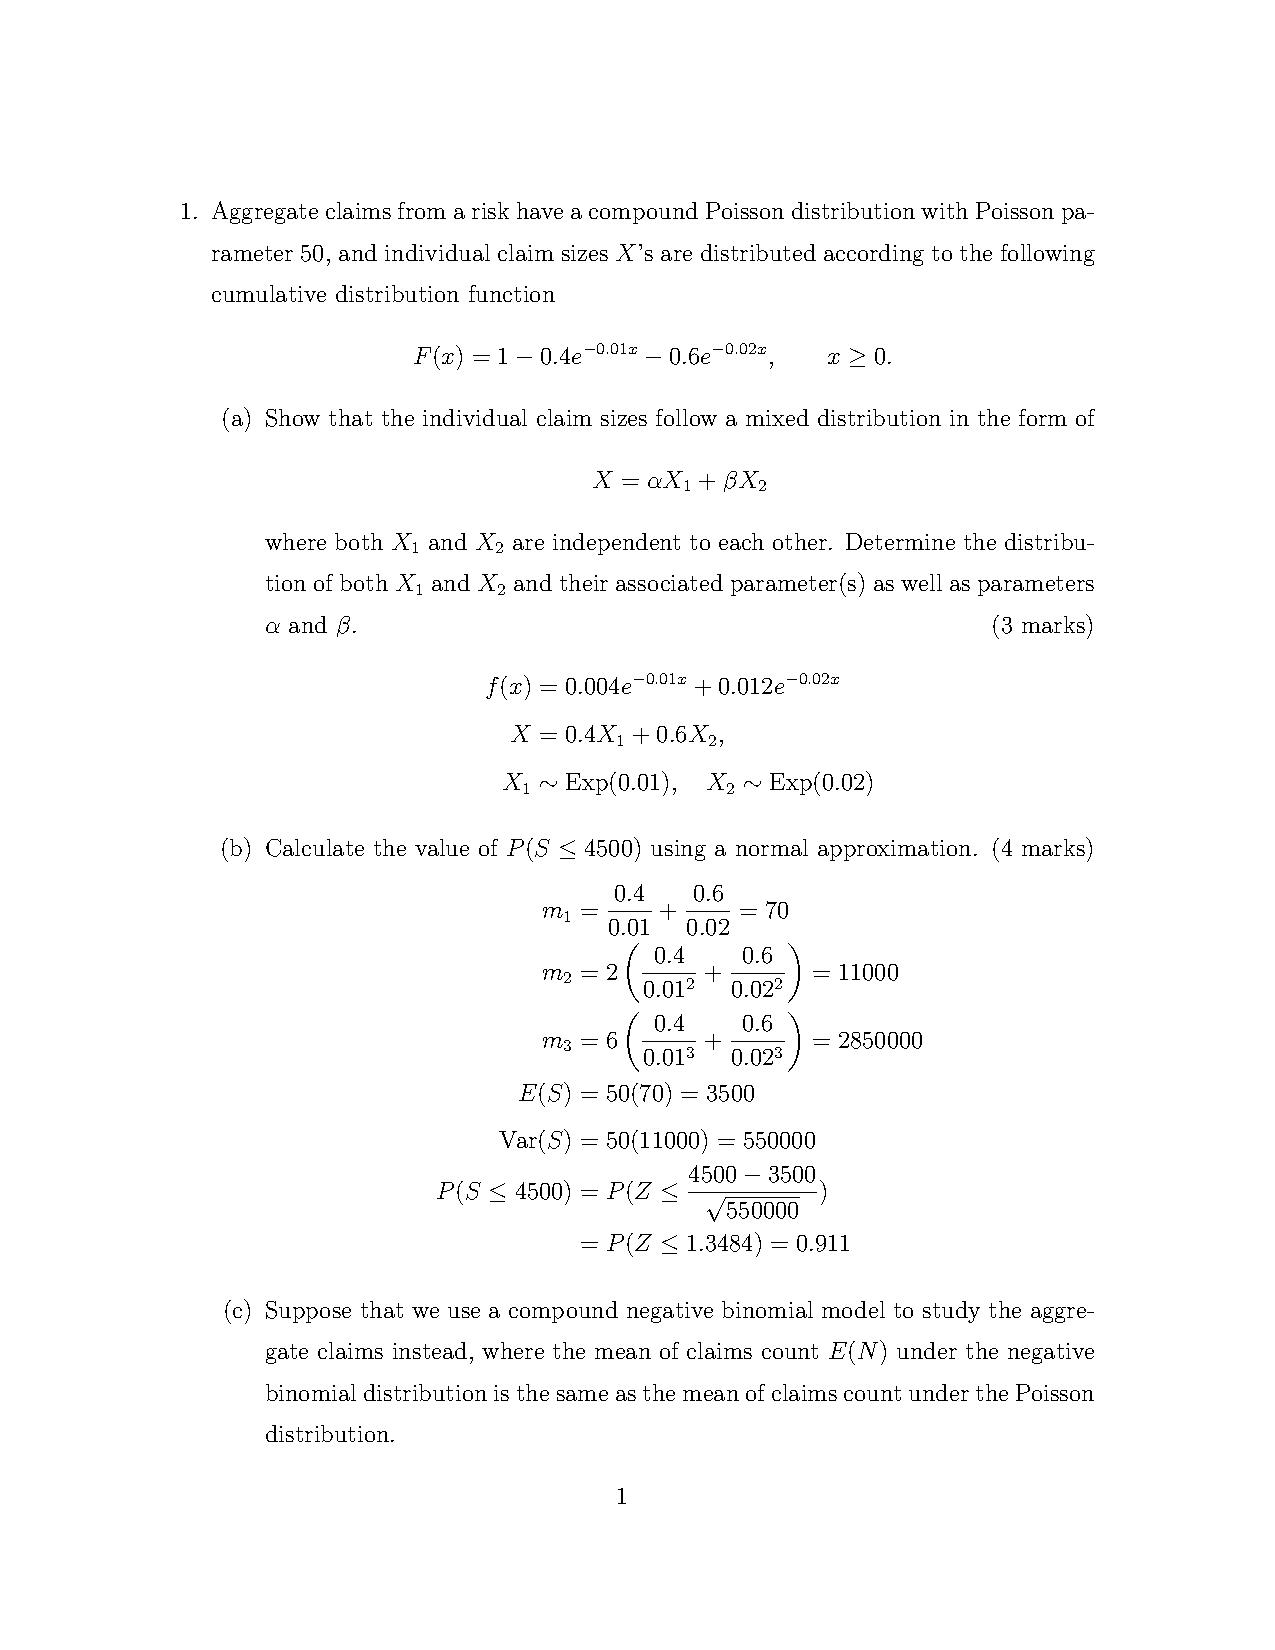
\includepdf[pages=-]{PracticeMST_2025_sol.pdf}

\section{Appendix F - MST Questions and Solutions}
$$\text{refer to next page}$$
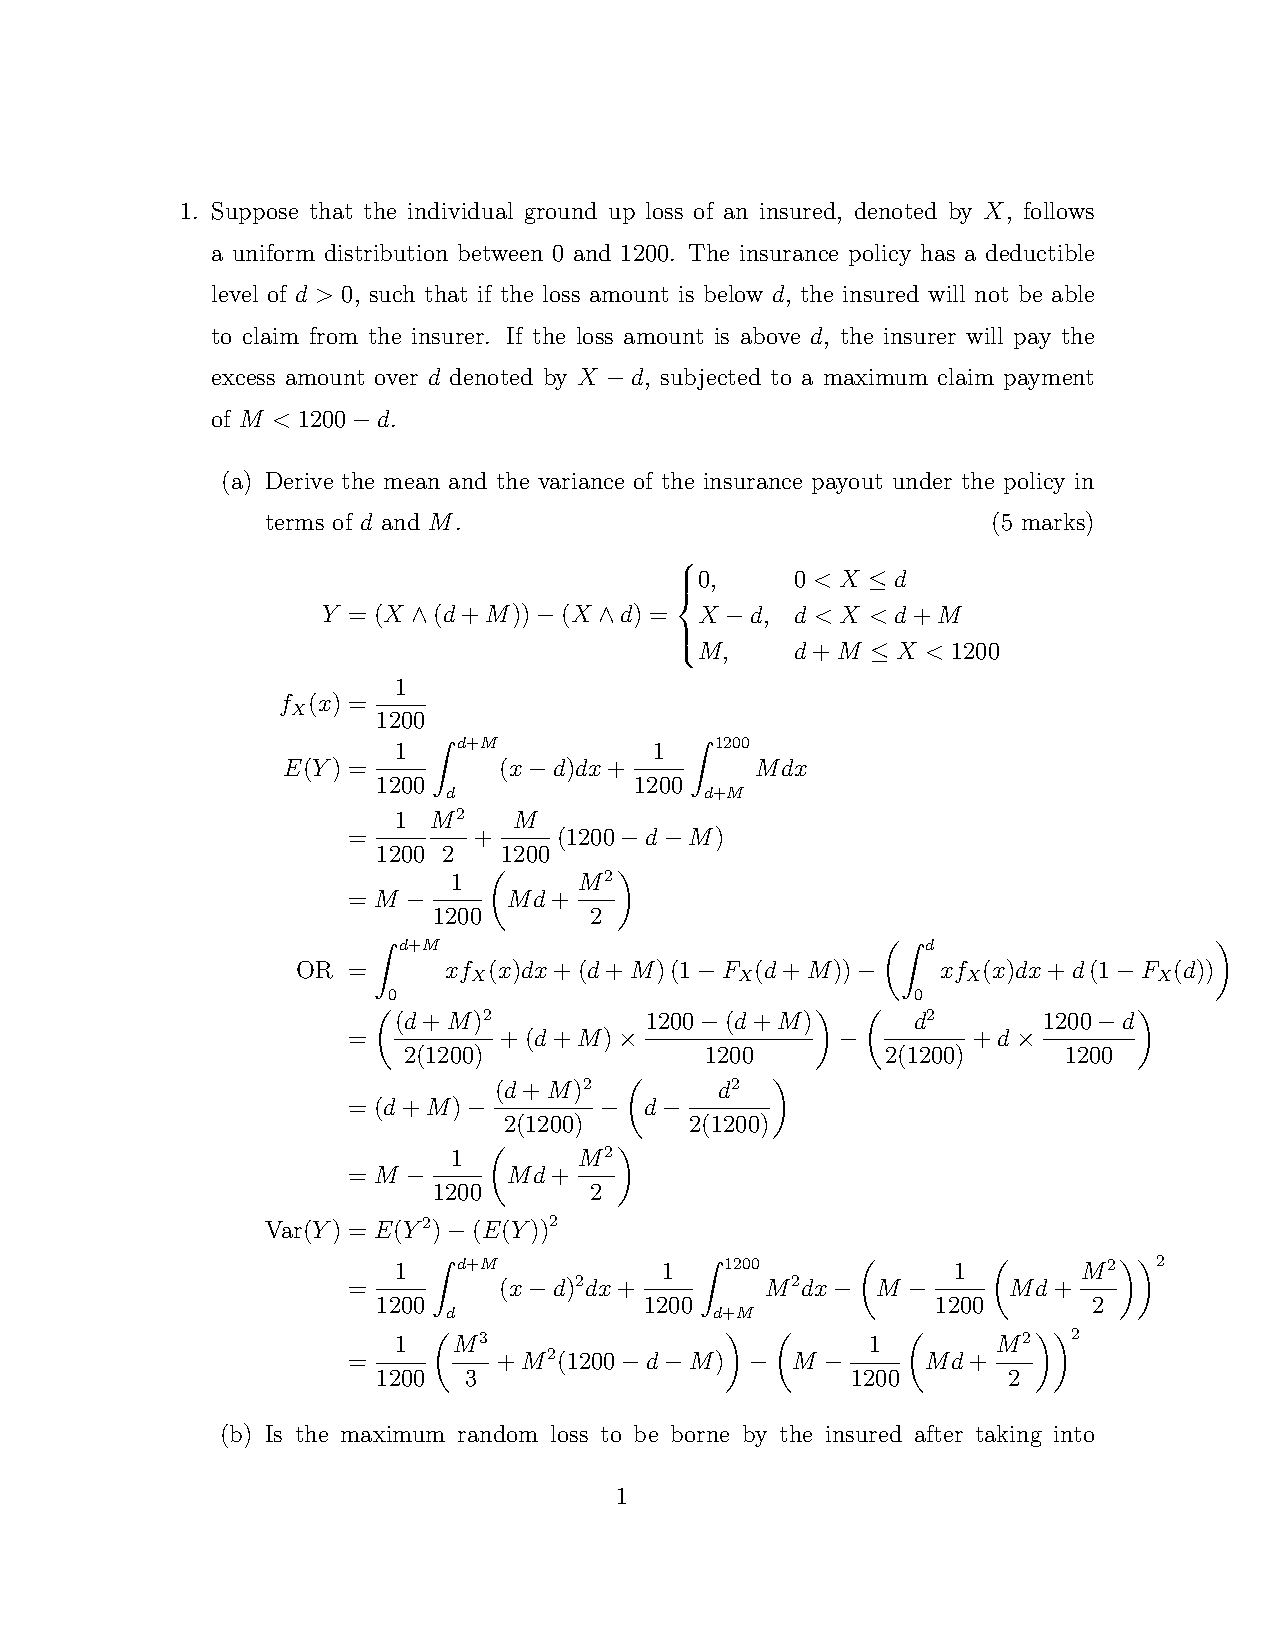
\includepdf[pages=-]{MST_2025_sol.pdf}

\section{Appendix G - Assignment R Code and Output}
$$\text{refer to next page}$$
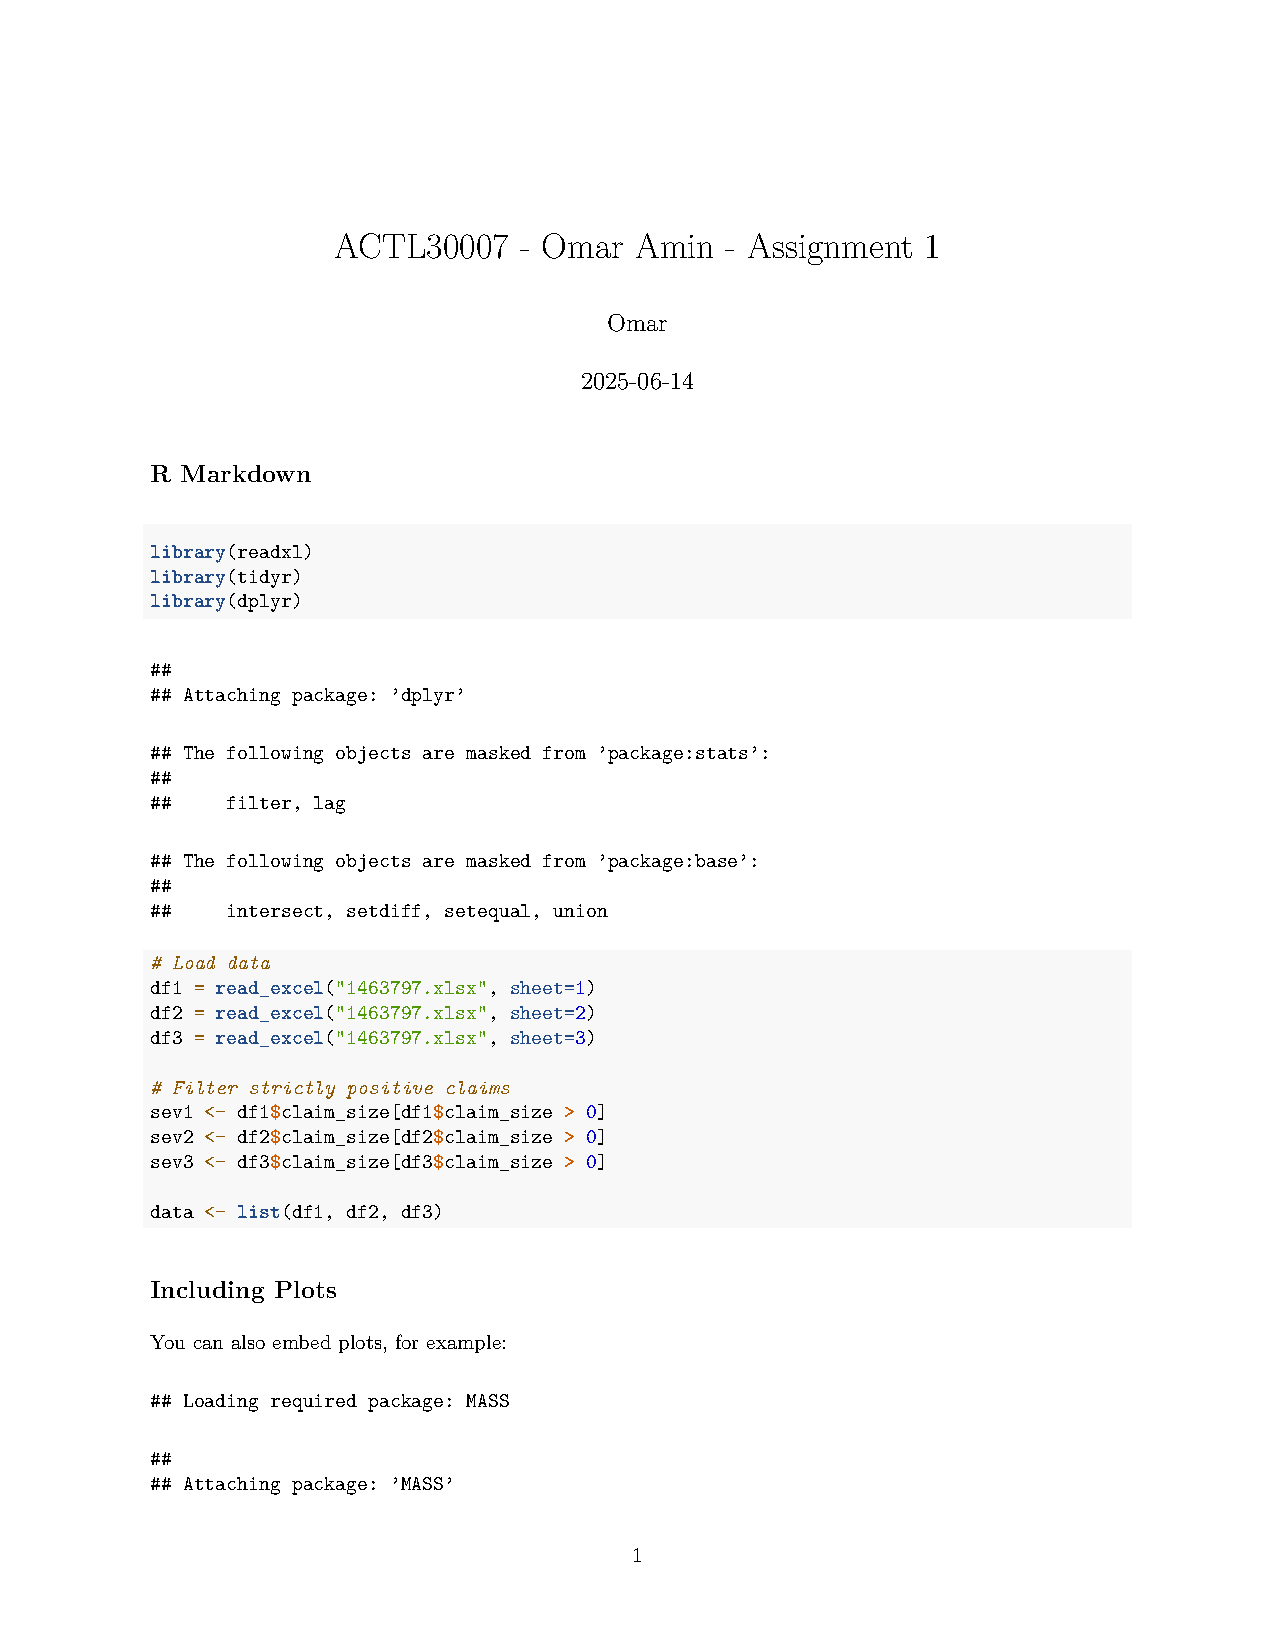
\includepdf[pages=-]{Assignment 1 - Knitted R Output.pdf}

\end{document}